\newpage
\chapter{RESULTADOS}

Con el objetivo de determinar la política de inventario óptima, se tuvo un registro de los productos de almacén, donde primero se analizó los productos más demandados, seguidamente se extrajo el monto total en soles de cada producto que tuvo en el año 2024 así como el respectivo volumen de almacenamiento que tiene en $cm^3$. Para que sean evaluados descriptivamente mediante el análisis ABC y el diagrama de Pareto, seleccionando los productos que se analizarán mediante el modelo de inventarios.

\section{Análisis descriptivo de los productos de almacén}

Primeramente se describirá los 471 productos registrados mediante el área y la especialidad indicando su porcentaje en costos y almacenamiento.

\subsection{Nivel de área}

En esta parte se describirá los resultados en porcentaje de los costos y almacenamiento de los productos agrupados por áreas.

\begin{table}[H]
    \caption{Resultados por área de productos de almacén}
    \begin{tabular}{p{2cm} p{2.51cm} p{4cm} p{4cm}} % Define anchos personalizados para cada columna
        \hline
        \textbf{Área} & \textbf{Productos} & \textbf{$(\%)$ de Costos} & \textbf{$(\%)$ Ocupación} \\
        \hline
        \textbf{Oftalmología} & 212 & $92.86\%$ & $80.09\%$ \\
        \textbf{Odontología} & 259 & $7.14\%$ & $19.91\%$ \\
        \hline
        \textbf{Total} & 471 & $100\%$ & $100\%$
    \end{tabular}
    \label{table:Area_productos}
\end{table}

La Tabla \ref{table:Area_productos} describe los 471 productos de almacén agrupados por área, se muestra que la mayor parte de costos son productos del área de oftalmología con 212 productos tomando el $92.86\%$ de costos, seguido del área de odontología con 259 productos tomando el $7.14\%$ de costos. De la misma forma el porcentaje de ocupación de productos de oftalmología es del $80.09\%$ mientras que productos del área de odontología ocupan solo el $19.91\%$ del espacio de almacén.

\subsection{Nivel de especialidad}

Se describirá los resultados con respecto al porcentaje de costos y espacio de almacenamiento de los productos agrupados por especialidad.

\subsubsection{Área de oftalmología}

En almacén con respecto a insumos del área de oftalmología se tienen registrado 212 productos los cuales sirven para abastecer las diferentes especialidades y servicios que ofrece el centro de salud integral del área de oftalmología, de los cuales estos vienen a ser:

\begin{itemize}
    \item Insumos generales
    \item Tintas (usadas para las impresoras que se tienen)
    \item INLASER
    \item FACO
    \item Retina
    \item CROSSLINKING
    \item Esterilización
    \item Catarata
    \item ICL
    \item Glaucoma
    \item Oculoplastía
    \item Avastin 
\end{itemize}

\newpage

\begin{table}[H]
    \caption{Resultados de insumos del área de oftalmología por especialidad}
    \begin{tabular}{p{4cm} p{2.5cm} p{3cm} p{3cm}} % Define anchos personalizados para cada columna
        \hline
        \textbf{Especialidad} & \textbf{Productos} & \textbf{$(\%)$ de Costos} & \textbf{$(\%)$ Ocupación} \\
        \hline
        \textbf{INLASER} & 6 & $39.27\%$ & $2.20\%$ \\
        \textbf{FACO} & 6 & $25.49\%$ & $2.82\%$ \\
        \textbf{Insumos generales} & 105 & $9.95\%$ & $31.91\%$ \\
        \textbf{Tintas} & 27 & $5.62\%$ & $6.38\%$ \\
        \textbf{Esterilización} & 27 & $3.66\%$ & $27.32\%$ \\
        \textbf{CROSSLINKING} & 2 & $3.09\%$ & $0.48\%$ \\
        \textbf{Catarata} & 10 & $2.10\%$ & $1.96\%$ \\
        \textbf{Retina} & 16 & $1.94\%$ & $4.60\%$ \\
        \textbf{Glaucoma} & 3 & $0.68\%$ & $0.37\%$ \\
        \textbf{Oculoplastía} & 6 & $0.58\%$ & $0.48\%$ \\
        \textbf{ICL} & 2 & $0.28\%$ & $0.34\%$ \\
        \textbf{Avastín} & 2 & $0.19\%$ & $1.22\%$ \\
        \hline
        \textbf{Total} & 212 & $92.86\%$ & $80.09\%$
    \end{tabular}
    \label{table:productos_oftalmologia}
\end{table}

La Tabla \ref{table:productos_oftalmologia} describe los productos del área de oftalmología agrupados por especialidad en donde se muestra que la mayor cantidad de productos del área de oftalmología son insumos generales con 105 productos ocupando el $31.91\%$ de almacén, seguido de 27 productos de la especialidad de esterilización ocupando el $27.32\%$ de almacén, tintas con 27 productos ocupando el $6.38\%$ de almacén, retina con 16 productos ocupando el $4.60\%$ de almacén, FACO con 6 productos ocupando el $2.82\%$ de almacén, INLASER con 6 productos ocupando el $2.20\%$ de almacén, catarata con 10 productos ocupando el $1.96\%$ de almacén, avastin con 2 productos ocupando el $1.22\%$ de almacén, oculoplastía con 6 productos ocupando el $0.48\%$ de almacén, CROSSLINKING con 2 productos ocupando el $0.48\%$ de almacén, glaucoma con 3 productos ocupando el $0.37\%$ de almacén, y los productos que ocupan el menor espacio en almacén son de la especialidad de ICL con 2 productos ocupando solo el $0.34\%$

\newpage

\begin{figure}[h!]
  \caption{Productos del área de oftalmología por especialidad en base al ($\%$) de costos}
  {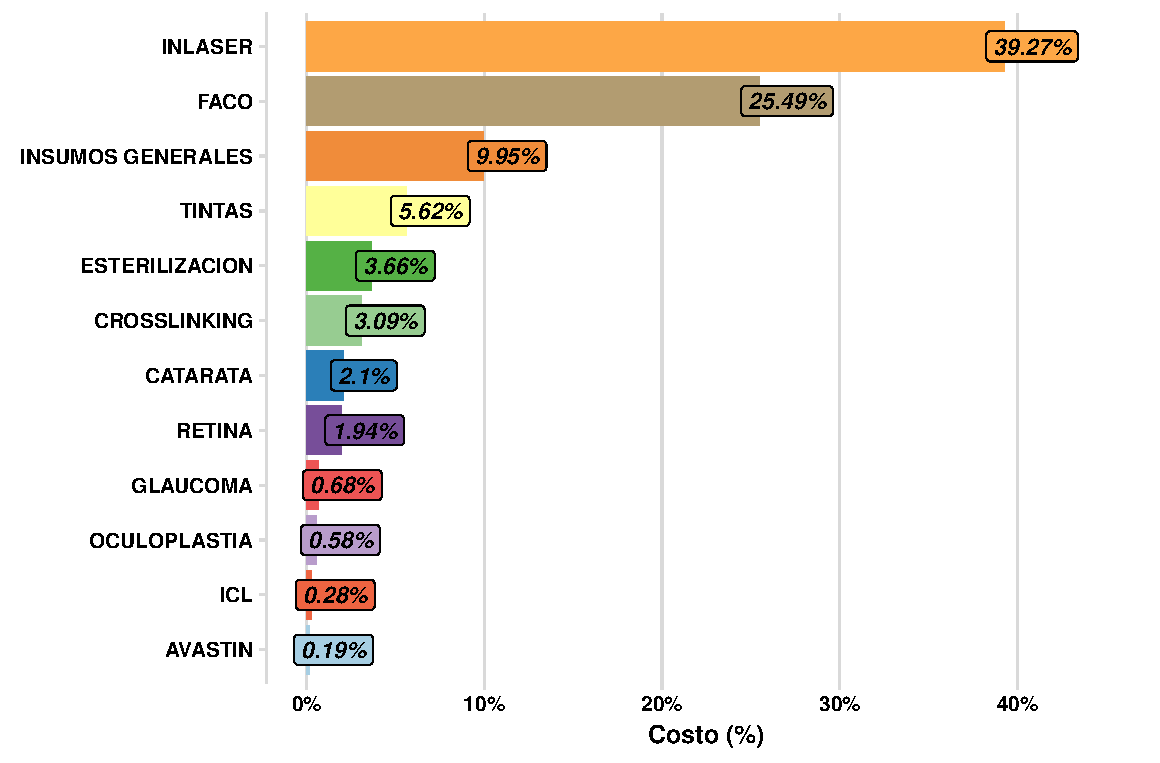
\includegraphics[width=15cm, height=10cm]{images/oftalm_prod.pdf}}
  \label{fig:Oftalm_espec}
\end{figure}

La Figura \ref{fig:Oftalm_espec} muestra un gráfico de barras de las especialidades del área de oftalmología ordenado por el porcentaje de costos, donde se observa que la mayor parte de los costos del área de oftalmología son de la especialidad de INLASER con el $39.27\%$ de los costos totales, seguido de la especialidad de FACO con el $25.49\%$ de costos, insumos generales con el $9.95\%$ de costos, tintas con el $5.62\%$ de costos, esterilización con el $3.66\%$ de costos, CROSSLINKING con $3.09\%$ de costos, catarata con $2.10\%$ de costos, retina con $1.94\%$ de costos, glaucoma con $0.68\%$ de costos, oculoplastía con $0.58\%$ de costos, ICL con $0.28\%$ de costos y de la especialidad de avastín con el $0.19\%$ de los costos totales.

\newpage

\subsubsection{Área de odontología}

En almacén con respecto a insumos del área de odontología se tienen registrado 260 productos los cuales sirven para abastecer las diferentes especialidades y servicios que ofrece el centro de salud integral en el área de odontología, de los cuales estos vienen a ser:

\begin{itemize}
    \item Prostodoncia
    \item Operatoria
    \item Endodoncia
    \item Cirugias
    \item Materiales
    \item Periodoncia
\end{itemize}

\begin{table}[H]
    \caption{Resultados de insumos del área de odontología por especialidad}
    \begin{tabular}{p{4cm} p{2.5cm} p{3cm} p{3cm}} % Define anchos personalizados para cada columna
        \hline
        \textbf{Especialidad} & \textbf{Productos} & \textbf{$(\%)$ de Costos} & \textbf{$(\%)$ Ocupación} \\
        \hline
        \textbf{Operatoria} & 93 & $2.09\%$ & $3.95\%$ \\
        \textbf{Prostodoncia} & 65 & $1.97\%$ & $4.24\%$ \\
        \textbf{Cirugías} & 16 & $1.28\%$ & $2.54\%$ \\
        \textbf{Materiales} & 25 & $0.92\%$ & $6.47\%$ \\
        \textbf{Endodoncia} & 51 & $0.68\%$ & $1.56\%$ \\
        \textbf{Periodoncia} & 9 & $0.19\%$ & $1.14\%$ \\
        \hline
        \textbf{Total} & 259 & $7.14\%$ & $19.91\%$
    \end{tabular}
    \label{table:productos_odontologia}
\end{table}

La Tabla \ref{table:productos_odontologia} describe los productos del área de odontología agrupados por especialidad, donde se muestra que la mayor cantidad de productos del área de odontología son materiales con 25 productos ocupando el $6.47\%$ de almacén, seguido de 65 productos de la especialidad de prostodoncia ocupando el $4.24\%$ de almacén, operatoria con 93 productos ocupando el $3.95\%$ de almacén, cirugías con 16 productos ocupando el $2.54\%$ de almacén, endodoncia con 51 productos ocupando el $1.56\%$ de almacén y periodoncia con 9 productos ocupando solo el $1.14\%$ de almacén.

\begin{figure}[H]
  \caption{Productos del área de odontología por especialidad en base al ($\%$) de costos}
  {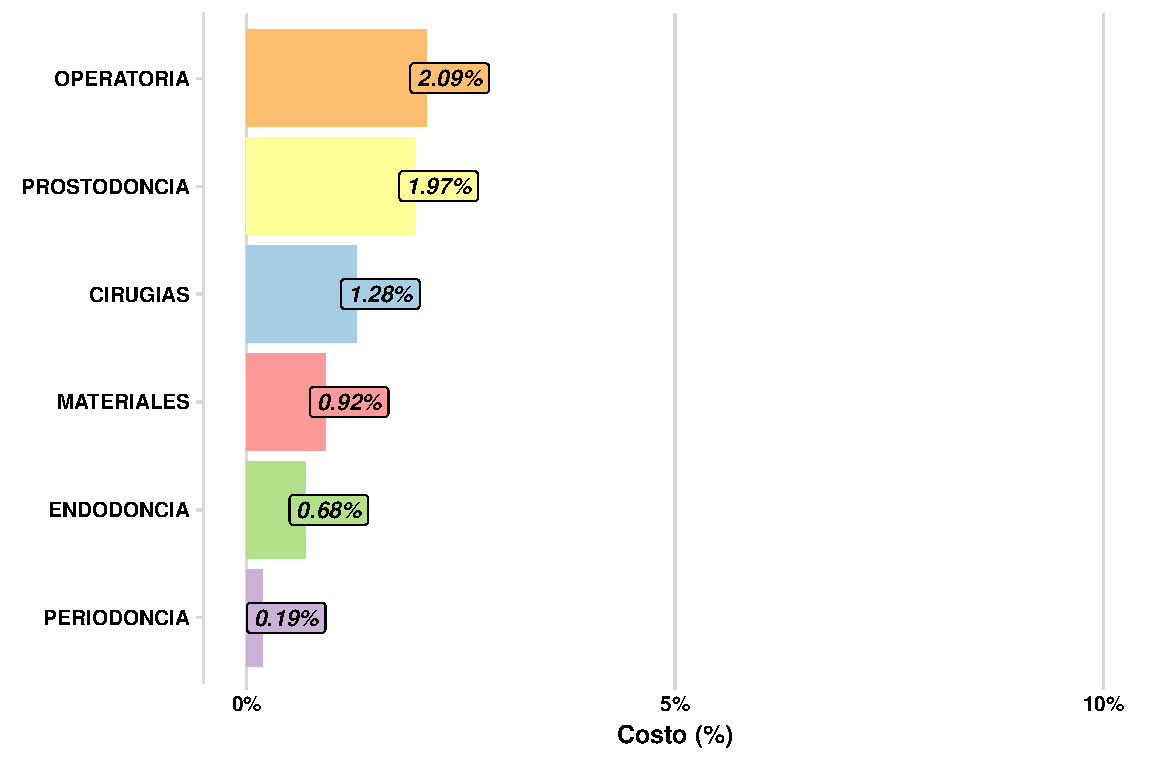
\includegraphics[width=15cm, height=10cm]{images/odonto_prod.pdf}}
  \label{fig:Odonto_espec}
\end{figure}

La Figura \ref{fig:Odonto_espec} muestra un gráfico de barras de las especialidades de odontología ordenados por el porcentaje de costos en donde se observa que la mayor parte de los costos del área de odontología son de la especialidad de operatoria con el $2.09\%$ de los costos totales, seguido de la especialidad de prostodoncia con el $1.97\%$ de costos, cirugías con $1.28\%$ de costos, materiales con $0.92\%$ de costos, endodoncia con $0.68\%$ de costos y de la especialidad de periodoncia con el $0.19\%$ de los costos totales.

\newpage

\section{Análisis descriptivo mediante actividades basadas en costos (ABC)}

Se describe la información de todos los productos registrados en función de los costos que vendrían a ser el costo total del año 2024 en salidas para evaluar la demanda en función monetaria, de la misma forma ver los espacios de almacenamiento. Este análisis será en función del porcentaje del total de costos y almacenamiento como se muestra en la Tabla \ref{table:ABC_resumen}

\begin{table}[H]
    \caption{Resultados de la clasificacìón (ABC)}
    \begin{tabular}{p{0.8cm} p{2.51cm} p{5.2cm} p{4.9cm}} % Define anchos personalizados para cada columna
        \hline
        \textbf{Grupo} & \textbf{Productos} & \textbf{$(\%)$ de Costos} & \textbf{$(\%)$ Ocupación} \\
        \hline
        \textbf{A} & 8 & $68.55\%$ & $3.74\%$ \\
        \textbf{B} & 34 & $21.36\%$ & $29.09\%$ \\
        \textbf{C} & 429 & $10.09\%$ & $67.17\%$ \\
        \hline
        \textbf{Total} & 471 & $100\%$ & $100\%$
    \end{tabular}
    \label{table:ABC_productos}
\end{table}

En la Tabla \ref{table:ABC_productos}, se muestra el análisis ABC de los productos de almacén del centro de salud clasificados mediante los costos producidos en el año 2024. De manera general se observa que la mayor denominación o cantidad de productos se encuentra en el grupo C con 429 productos ocupando el $67.17\%$ del espacio de almacén, seguido del grupo B con 34 productos ocupando el $29.09\%$ del espacio de almacén y por último el grupo A con 8 productos ocupando solo el $3.74\%$ del espacio de almacén.

\newpage
\begin{figure}[H]
  \caption{Diagrama de Pareto productos de almacén del centro de salud integral agrupados por análisis basados en costos (ABC)}
  {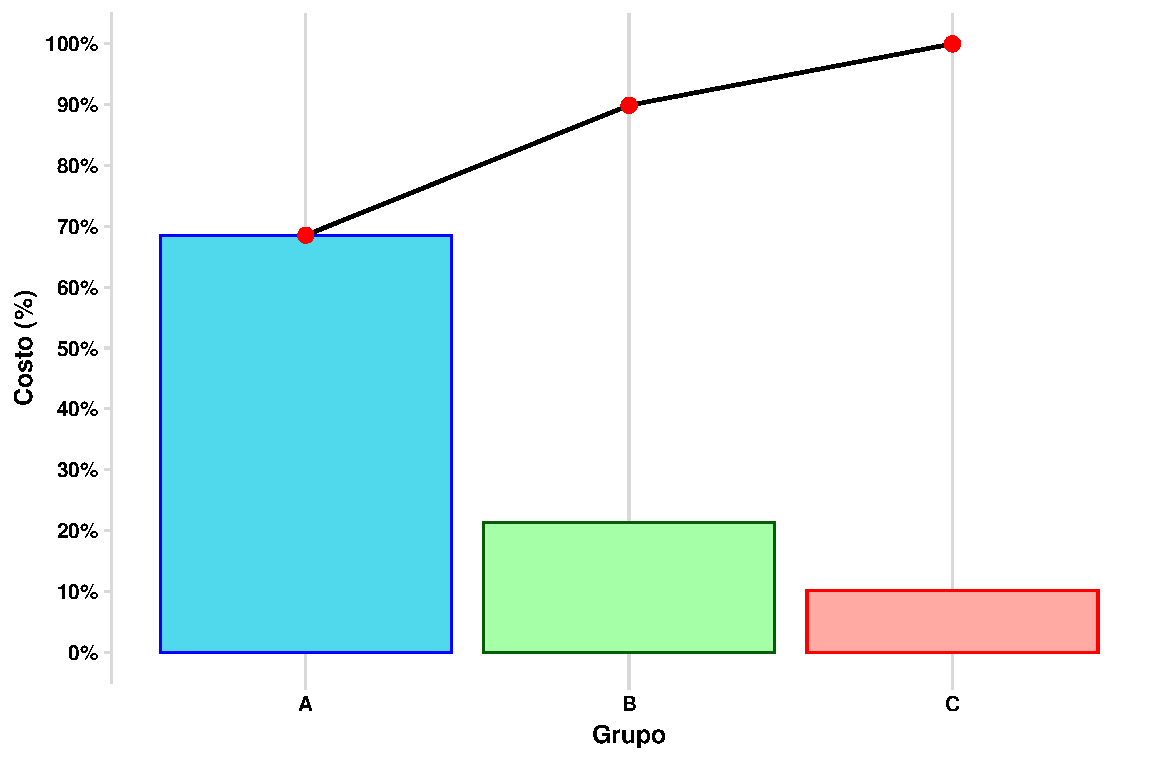
\includegraphics[width=15cm, height=7.9cm]{images/ABC.pdf}}
  \label{fig:ABC_almacen}
\end{figure}

En la Figura \ref{fig:ABC_almacen} se observa el diagrama de Pareto con respecto a los costos acumulados en el año 2024 de los productos de almacén del centro de salud integral, en donde se observa que los 8 productos del grupo A conforman un $68.55\%$ de los costos totales de almacén, los del grupo B el $21.36\%$ y los del grupo C solo el $10.09\%$ de costos totales.

\subsection{Selección de productos}

Tomando en cuenta los resultados de la Tabla \ref{table:ABC_productos} y el diagrama de Pareto de la Figura \ref{fig:ABC_almacen}, la política de inventarios debe priorizar a los 8 productos que se encuentran en el grupo A del análisis ABC. Siguiendo la metodología ABC de la sección (\ref{section:ABC}) se tomará los 8 productos del grupo A y productos del grupo B que tienen mayores costos, esto con la solicitud del área de logística del centro de salud siendo 10 productos adicionales. Teniendo un total de 18 productos seleccionados en los que se aplicarán los modelos de inventarios.

\subsubsection{Resultados descriptivos de productos seleccionados}

Se describirá los resultados con respecto al porcentaje de costos y espacio de almacenamiento de los productos seleccionados para el modelo de inventarios.

\begin{table}[H]
    \caption{Resultados por área de productos seleccionados mediante el análisis ABC}
    \begin{tabular}{p{2cm} p{2.51cm} p{4cm} p{4cm}} % Define anchos personalizados para cada columna
        \hline
        \textbf{Área} & \textbf{Productos} & \textbf{$(\%)$ de Costos} & \textbf{$(\%)$ Ocupación} \\
        \hline
        \textbf{Oftalmología} & 18 & $79.31\%$ & $24.44\%$ \\
        \hline
    \end{tabular}
    \label{table:GrupoA_Area_Productos}
\end{table}

La Tabla \ref{table:GrupoA_Area_Productos} muestra los productos seleccionados mediante el análisis ABC agrupados por área, en el que todos los 18 productos seleccionados son del área de oftalmología ocupando el $79.31\%$ de costos y ocupan un $24.44\%$ del espacio de almacén.

\begin{table}[H]
    \caption{Resultados por especialidad de productos seleccionados mediante el análisis ABC}
    \begin{tabular}{p{2.5cm} p{3cm} p{2cm} p{3cm} p{3cm}}
        \hline
        \textbf{Área} & \textbf{Especialidad} & \textbf{Productos} & \textbf{$(\%)$ de Costos} & \textbf{$(\%)$ Ocupación} \\
        \hline
        \multirow{7}{*}{\textbf{Oftalmología}} & \textbf{INLASER} & 2 & $39.27\%$ & $0.79\%$ \\ \cline{2-5}
        & \textbf{FACO} & 5 & $25.49\%$ & $2.59\%$ \\ \cline{2-5}
        & \textbf{Insumos generales} & 4 & $5.97\%$ & $1.49\%$ \\ \cline{2-5}
        & \textbf{Tintas} & 3 & $3.78\%$ & $0.86\%$ \\ \cline{2-5} \cline{2-5}
        & \textbf{CROSSLINKING} & 1 & $2.58\%$ & $0.24\%$ \\ \cline{2-5}
        & \textbf{Catarata} & 2 & $1.52\%$ & $0.76\%$ \\ \cline{2-5}
        & \textbf{Esterilización} & 1 & $0.71\%$ & $17.70\%$ \\
        \hline
        \multicolumn{2}{c}{\textbf{Total}} & 18 & $79.31\%$ & $24.44\%$ 
    \end{tabular}
    \label{table:GrupoA_Especialidad}
\end{table}

La Tabla \ref{table:GrupoA_Especialidad} muestra los productos seleccionados mediante el análisis ABC agrupados por especialidad, en donde se muestra que la mayor parte de los productos seleccionados por el análisis ABC son de la especialidad de INLASER con 2 productos ocupando el $39.27\%$ de costos, seguido de 5 productos de la especialidad de FACO ocupando el $2.59\%$ de costos, insumos generales con 4 productos ocupando el $1.49\%$ de costos, tintas con 3 productos ocupando el $3.78\%$ de costos, CROSSLINKING con 1 producto ocupando el $2.58\%$ de costos, catarata con 2 productos ocupando el $1.52\%$ de costos y esterilización con 1 producto ocupando el $0.71\%$ de costos. De la misma forma que con respecto al porcentaje de ocupación de almacén, el producto de esterilización ocupan una gran parte de almacén siendo el $17.70\%$ del área de almacén, y los que ocupan la menor parte es el producto de CROSSLINKING con solo el $0.24\%$ de ocupación de almacén.

\begin{figure}[h!]
  \caption{Productos seleccionados mediante el análisis ABC por especialidad en base al ($\%$) de costos}
  {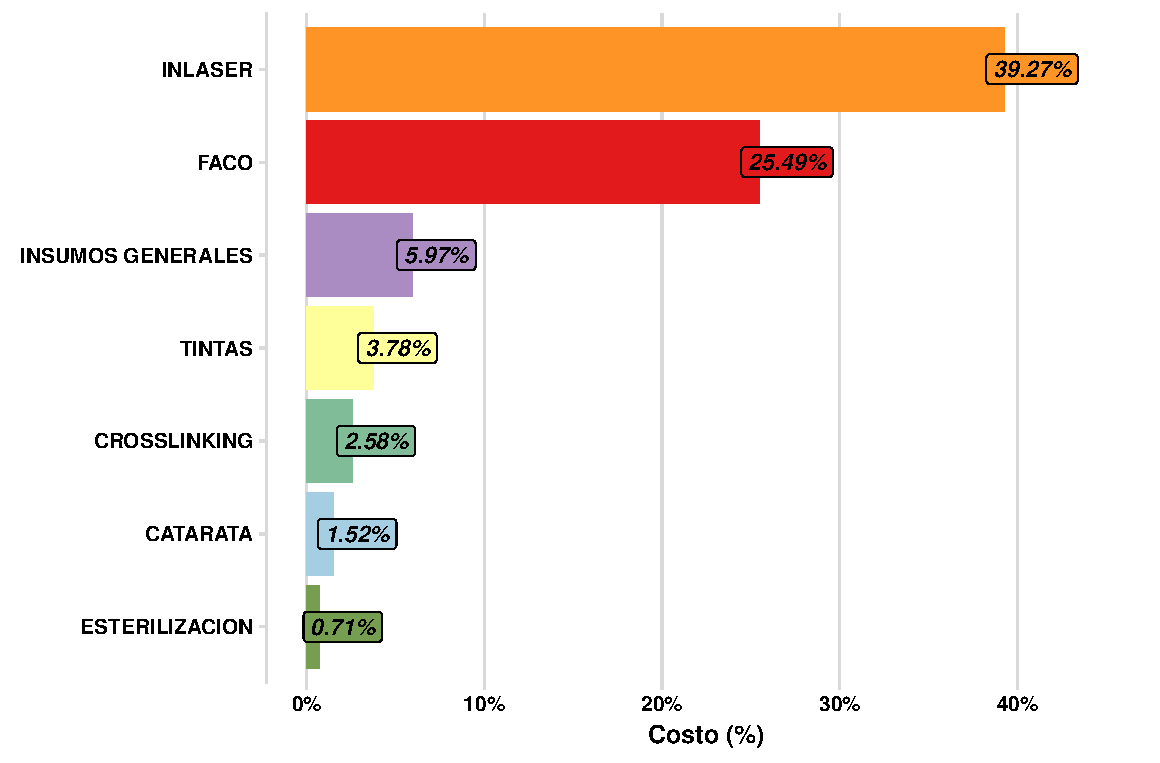
\includegraphics[width=15cm, height=10cm]{images/Especialidad.pdf}}
  \label{fig:EspecialidadGrupoA_almacen}
\end{figure}

La Figura \ref{fig:EspecialidadGrupoA_almacen} muestra un diagrama de barras de los productos seleccionados mediante el análisis ABC agrupados por especialidad y ordenados en base al porcentaje al costo, se observa que de los productos seleccionados para aplicar el modelo de inventarios lo que tienen la mayor parte de costos son de la especialidad de INLASER siendo el $39.27\%$ de los costos, seguido de FACO con el $25.49\%$ de costos, mientras que los productos con menor porcentaje son de la especialidad de CROSSLINKING, catarata y esterilización.

\newpage
\subsubsection{Descripción de los productos seleccionados}

\begin{longtable}{p{2cm} p{2cm} p{3.1cm} p{6.5cm}}
    \caption{Descripción de los productos seleccionados mediante la clasificacìón (ABC)}
    \label{table:ABC_productos_desc} \\
        \hline

        \hline
    \textbf{Código} & \textbf{Área} & \textbf{Subárea} & \textbf{Denominación} \\
        \hline
    \hline
    \endfirsthead

    \hline
    \textbf{Código} & \textbf{Área} & \textbf{Subárea} & \textbf{Denominación} \\
        \hline
    \hline
    %\multicolumn{5}{l}{\textbf{Independiente}} \\ % Se repite al inicio de cada nueva página
    \hline
    \endhead

    \hline
    \endfoot

    \hline
    \endlastfoot

        \hline
        \textbf{PROD001} & Oftalmología & INLASER & Paquete de tratamiento talla ``S'' \\
        \textbf{PROD002} & Oftalmología & FACO & KIT para procedimiento quirúrgico oftálmico (pack centurion ultra balance) \\
        \textbf{PROD003} & Oftalmología & FACO & Bolsa de solución BSS BAG 500 ml \\
        \textbf{PROD004} & Oftalmología & FACO & Cuchillo de hendidura CLEAR CUT HP2 2.4 mm bisel doble, intrepido sistema microcoaxial \\
        \textbf{PROD005} & Oftalmología & FACO & AJL VISC 1.4$\%$ - pack solución viscoelástica para uso intraocular hialuronato sódico 14 mg/ml canula 1x27g \\
        \textbf{PROD006} & Oftalmología & Insumos generales & Cuchillo lateral CLEAR CUT doble bisel 1.2 mm angulado \\
        \textbf{PROD007} & Oftalmología & CROSSLINKING & Solución de riboflavina VIBEX RAPID 0.1$\%$ isotonico jeringa de 1.5 ml \\
        \textbf{PROD008} & Oftalmología & INLASER & Anterior chamber cannula 27 g x 9 mm BEND \\
        \textbf{PROD009} & Oftalmología & FACO & Canula para cistotoma formada 27 g \\
        \textbf{PROD010} & Oftalmología & Tintas & Toner TNP80Y yellow para Konica Minolta BIZHUB C-3320i \\
        \textbf{PROD011} & Oftalmología & Insumos generales & Campo quirúrgico para ojos desechable 100 cm x 70 cm \\
        \textbf{PROD012} & Oftalmología & Tintas & Toner TNP80C cyan para Konica Minolta BIZHUB C-3320i \\
        \textbf{PROD013} & Oftalmología & Insumos generales & Lentes de contacto - AIR optix dia y noche \\
        \textbf{PROD014} & Oftalmología & Tintas & Toner Konica Minolta BIZHUB C-3320i Magenta \\
        \textbf{PROD015} & Oftalmología & Catarata & Solución salina equilibrada (BSS) en botella de vidrio 500 ml \\
        \textbf{PROD016} & Oftalmología & Insumos generales & Campo quirúrgico 100 x 120 cm \\
        \textbf{PROD017} & Oftalmología & Catarata & Azul de tripan 0.06$\%$ - 0.6 mg VIAL x 1 ml / OCUBLU - TRY \\
        \textbf{PROD018} & Oftalmología & Esterilización & Agua destilada y/o desionizada \\
        \hline
\end{longtable}

La Tabla \ref{table:ABC_productos_desc} muestra la descripción de los productos seleccionados mediante la clasificación (ABC), así como del área y subárea correspondiente. La mayor parte de las denominaciones vienen a ser instrumentos utilizados en las cirugías realizadas por el centro de salud integral ``La Fuente'' en el área de oftalmología; asimismo también se tienen productos utilizados por impresoras ya sea en la impresión de exámenes y evaluaciones realizadas.  

\section{Análisis de la demanda y selección del modelo}

Evaluando el KARDEX se tiene que los productos evaluados son mayormente derivados al área de sala de cirugías de oftalmología (a excepción de TINTAS), en el cual el área indica que el uso de los productos es según a las cirugías realizadas (cada producto utilizado para diferentes tipos de cirugías) no contando por el momento un registro de utilización de los productos, por el cual la estimación de la demanda de los productos se realizará en base a las cirugías realizadas del centro de salud en el año 2024.

Estableciendo un periodo de tiempo de 1 año tomando en cuenta las demandas mensuales en el año 2024 de los 18 productos seleccionados, se presenta la siguiente Tabla.

\newpage
\begin{landscape}

\begin{table}[H]
    \caption{Demanda mensual del año 2024 de los productos seleccionados}
    \footnotesize
    \begin{tabular}{p{1cm} >{\centering\arraybackslash}p{1.2cm} >{\centering\arraybackslash}p{1.2cm} >{\centering\arraybackslash}p{1.2cm} >{\centering\arraybackslash}p{1.2cm} >{\centering\arraybackslash}p{1.2cm} >{\centering\arraybackslash}p{1.2cm} >{\centering\arraybackslash}p{1.2cm} >{\centering\arraybackslash}p{1.2cm} >{\centering\arraybackslash}p{1.2cm} >{\centering\arraybackslash}p{1.2cm} >{\centering\arraybackslash}p{1.2cm} >{\centering\arraybackslash}p{1.2cm} } % Define anchos personalizados para cada columna
        \hline
        \textbf{Código} & \textbf{Enero} & \textbf{Febrero} & \textbf{Marzo} & \textbf{Abril} & \textbf{Mayo} & \textbf{Junio} & \textbf{Julio} & \textbf{Agosto} & \textbf{Setiembre} & \textbf{Octubre} & \textbf{Noviembre} & \textbf{Diciembre} \\
        \hline
        \textbf{PROD001} & 53 & 44 & 8 & 31 & 16 & 35 & 21 & 58 & 34 & 39 & 50 & 20 \\
        \textbf{PROD002} & 7 & 8 & 7 & 11 & 4 & 7 & 8 & 8 & 9 & 8 & 8 & 7 \\
        \textbf{PROD003} & 20 & 25 & 26 & 34 & 19 & 28 & 33 & 30 & 30 & 30 & 28 & 18 \\
        \textbf{PROD004} & 36 & 50 & 53 & 62 & 32 & 55 & 64 & 55 & 58 & 59 & 52 & 36 \\
        \textbf{PROD005} & 37 & 50 & 53 & 62 & 32 & 55 & 64 & 56 & 59 & 59 & 53 & 36 \\
        \textbf{PROD006} & 36 & 50 & 53 & 62 & 32 & 55 & 64 & 55 & 58 & 59 & 52 & 36 \\
        \textbf{PROD007} & 2 & 7 & 4 & 4 & 2 & 3 & 8 & 7 & 7 & 5 & 4 & 4 \\
        \textbf{PROD008} & 20 & 24 & 4 & 16 & 6 & 14 & 12 & 17 & 12 & 17 & 20 & 7 \\
        \textbf{PROD009} & 36 & 50 & 53 & 62 & 32 & 55 & 64 & 55 & 58 & 59 & 52 & 36 \\
        \textbf{PROD010} & 1 & 1 & 1 & 1 & 1 & 1 & 2 & 1 & 1 & 1 & 1 & 1 \\
        \textbf{PROD011} & 54 & 69 & 66 & 72 & 43 & 73 & 78 & 76 & 71 & 77 & 69 & 50 \\
        \textbf{PROD012} & 1 & 1 & 1 & 1 & 1 & 1 & 1 & 1 & 2 & 1 & 1 & 1 \\
        \textbf{PROD013} & 17 & 17 & 11 & 12 & 9 & 16 & 11 & 19 & 13 & 13 & 14 & 7 \\
        \textbf{PROD014} & 1 & 1 & 1 & 2 & 1 & 1 & 1 & 1 & 2 & 1 & 1 & 1 \\
        \textbf{PROD015} & 11 & 14 & 11 & 16 & 8 & 12 & 14 & 14 & 16 & 15 & 16 & 12 \\
        \textbf{PROD016} & 41 & 63 & 60 & 65 & 39 & 64 & 78 & 65 & 69 & 68 & 70 & 47 \\
        \textbf{PROD017} & 30 & 29 & 40 & 55 & 24 & 47 & 53 & 46 & 51 & 45 & 47 & 27 \\
        \textbf{PROD018} & 6 & 8 & 7 & 6 & 3 & 4 & 8 & 5 & 9 & 5 & 9 & 6 \\
        \hline
    \end{tabular}
    \label{table:Demanda_ABC_productos}
\end{table}

\end{landscape}

La Tabla \ref{table:Demanda_ABC_productos} muestra la demanda por los 12 meses de los productos seleccionados en el año 2024. 

Posteriormente se hallará el coeficiente de variabilidad ($CV$) mediante la ecuación (\ref{CVar}), como asi mismo se determinará el modelo de inventarios adecuado.

\begin{table}[H]
    \caption{Coeficiente de variabilidad y modelo de inventarios de los productos seleccionados}
    \begin{tabular}{p{2cm} p{2cm} p{2cm} p{2cm} p{2cm} p{2.5cm}} % Define anchos personalizados para cada columna
        \hline
        \textbf{Código} & \textbf{Total} & \textbf{$Media$} & \textbf{$Varianza$} & \textbf{$CV$} & \textbf{Modelo} \\
        \hline
        \textbf{PROD001} & 409 & $34.08$ & $224.41$ & $0.19$ & \textbf{Determinístico} \\
        \textbf{PROD002} & 92 & $7.67$ & $2.39$ & $0.04$ & \textbf{Determinístico} \\
        \textbf{PROD003} & 321 & $26.75$ & $26.02$ & $0.04$ & \textbf{Determinístico} \\
        \textbf{PROD004} & 612 & $51.00$ & $104.33$ & $0.04$ & \textbf{Determinístico} \\
        \textbf{PROD005} & 616 & $51.33$ & $104.06$ & $0.04$ & \textbf{Determinístico} \\
        \textbf{PROD006} & 612 & $51.00$ & $104.33$ & $0.04$ & \textbf{Determinístico} \\
        \textbf{PROD007} & 57 & $4.75$ & $3.85$ & $0.17$ & \textbf{Determinístico} \\
        \textbf{PROD008} & 169 & $14.08$ & $34.58$ & $0.17$ & \textbf{Determinístico} \\
        \textbf{PROD009} & 612 & $51.00$ & $104.33$ & $0.04$ & \textbf{Determinístico} \\
        \textbf{PROD010} & 13 & $1.08$ & $0.08$ & $0.07$ & \textbf{Determinístico} \\
        \textbf{PROD011} & 798 & $66.50$ & $118.25$ & $0.03$ & \textbf{Determinístico} \\
        \textbf{PROD012} & 13 & $1.08$ & $0.08$ & $0.07$ & \textbf{Determinístico} \\
        \textbf{PROD013} & 159 & $13.25$ & $11.52$ & $0.07$ & \textbf{Determinístico} \\
        \textbf{PROD014} & 14 & $1.17$ & $0.14$ & $0.10$ & \textbf{Determinístico} \\
        \textbf{PROD015} & 159 & $13.25$ & $5.69$ & $0.03$ & \textbf{Determinístico} \\
        \textbf{PROD016} & 729 & $60.75$ & $134.02$ & $0.04$ & \textbf{Determinístico} \\
        \textbf{PROD017} & 494 & $41.17$ & $108.64$ & $0.06$ & \textbf{Determinístico} \\
        \textbf{PROD018} & 76 & $6.33$ & $3.39$ & $0.08$ & \textbf{Determinístico} \\
        \hline
    \end{tabular}
    \label{table:GrupoA_Area}
\end{table}

La Tabla \ref{table:GrupoA_Area} muestra el coeficiente de variabilidad calculado para los productos seleccionados. Donde se muestra que todos los productos tienen una demanda determinística ya que su coeficiente de variabilidad es menor a 0.20 en lo que se usará un modelo determinístico de inventarios.

\section{Determinación de costos}

Procedamos a recopilar la información de los costos. El área de administración y logística proporcionó la información de compras y factores asociados al almacén del centro de salud. Para esta parte tomemos los productos seleccionados mediante el análisis ABC presentado en la sección anterior, seguidamente hallemos los costos específicos de cada producto, que se presentará en cada subsección a continuación, de la misma forma será en tamaño de su ocupación en el área de almacén, que se presenta en la siguiente Tabla.

\begin{table}[H]
    \caption{Ocupación de los productos seleccionados mediante el análisis ABC}
    \begin{tabular}{p{2cm} p{3cm} p{5cm}} % Define anchos personalizados para cada columna
        \hline
        \textbf{Código} & \textbf{Volumen ($cm^3$)} & \textbf{Proporción en almacén} \\
        \hline
        \textbf{PROD001} & 42400 & $0.3367\%$ \\
        \textbf{PROD002} & 63920 & $0.5077\%$ \\
        \textbf{PROD003} & 140296 & $1.1142\%$ \\
        \textbf{PROD004} & 28800 & $0.2287\%$ \\
        \textbf{PROD005} & 52800 & $0.4193\%$ \\
        \textbf{PROD006} & 54720 & $0.4346\%$ \\
        \textbf{PROD007} & 30720 & $0.2440\%$ \\
        \textbf{PROD008} & 57600 & $0.4575\%$ \\
        \textbf{PROD009} & 40700 & $0.3232\%$ \\
        \textbf{PROD010} & 36000 & $0.2859\%$ \\
        \textbf{PROD011} & 92800 & $0.7370\%$ \\
        \textbf{PROD012} & 36000 & $0.2859\%$ \\
        \textbf{PROD013} & 29700 & $0.2359\%$ \\
        \textbf{PROD014} & 36000 & $0.2859\%$ \\
        \textbf{PROD015} & 85280 & $0.6773\%$ \\
        \textbf{PROD016} & 10640 & $0.0845\%$ \\
        \textbf{PROD017} & 10800 & $0.0858\%$ \\
        \textbf{PROD018} & 2228696 & $17.70\%$ \\
        \hline
    \end{tabular}
    \label{table:GrupoA_Ocupacion}
\end{table}

La Tabla \ref{table:GrupoA_Ocupacion} muestra los productos seleccionados con respecto a la dimensión que ocupa en el área de almacén. El volumen considera el espacio que se esta asignando para cada producto de almacén independientemente si los productos ocupan todo o parte del espacio asignado. No se mostraron costos de escasez ya que se tuvieron todos los productos para satisfacer la demanda en el año 2024, por lo que se tomarán los costos de compra, costo de preparación y costo de almacenamiento.

\subsection{Costo de compra}
Como se definió en la ecuación (\ref{2.1}) este viene a ser los costos por unidad de cada artículo del inventario, en el cual se debe incluir costos de descuento. En la política de inventario el costo de compra no influye, pero si influye en el costo total de cada producto.

Para determinar este costo, se tomó en cuenta el KARDEX de logística en el cual se precisa el precio unitario de cada producto. Mediante la consulta al área de logística se indicó que los precios de cada producto ya son determinados de manera fija por previo acuerdo con el proveedor independiente de un descuento por cantidad, asimismo este precio de pedido también incluye el precio de transporte. Lo que indica que los precios de compra son únicamente los precios unitarios de cada producto registrado en el KARDEX resumido de la siguiente forma:
\begin{itemize}
\item \textbf{Costo de compra:} Costo de adquirir el producto, de manera fija con previo acuerdo del proveedor por lo que no tiene descuento.
\item \textbf{Costo de transporte:} No esta incluido ya que el acuerdo de pedido es independiente a los costos de transporte, es decir se puede realizar el pedido de $n$ productos sin necesidad de que haya un costo adicional de transporte.
\end{itemize}

La información de los productos seleccionados mediante el análisis ABC se muestra en la siguiente Tabla.

\newpage
\begin{table}[H]
    \caption{Costos de compra de los productos seleccionados mediante el análisis ABC}
    \begin{tabular}{p{2cm} p{5cm} p{6.5cm}} % Define anchos personalizados para cada columna
        \hline
        \textbf{Código} & \textbf{Costo Unitario (S/)} & \textbf{Costo total del año 2024 (S/)} \\
        \hline
        \textbf{PROD001} & S/ 4,282.68 & S/ 165,471.40 \\
        \textbf{PROD002} & S/ 542.60 & S/ 49,666.90 \\
        \textbf{PROD003} & S/ 345.15 & S/ 21,532.12 \\
        \textbf{PROD004} & S/ 69.80 & S/ 17,572.86 \\
        \textbf{PROD005} & S/ 90.00 & S/ 17,100.00 \\
        \textbf{PROD006} & S/ 72.81 & S/ 11,828.01 \\
        \textbf{PROD007} & S/ 362.94 & S/ 11,370.00 \\
        \textbf{PROD008} & S/ 16.00 & S/ 7,680.00 \\
        \textbf{PROD009} & S/ 143.00 & S/ 6,507.00 \\
        \textbf{PROD010} & S/ 720.00 & S/ 6,498.00 \\
        \textbf{PROD011} & S/ 15.59 & S/ 6,259.82 \\
        \textbf{PROD012} & S/ 715.00 & S/ 5,839.00 \\
        \textbf{PROD013} & S/ 143.37 & S/ 4,874.58 \\
        \textbf{PROD014} & S/ 715.00 & S/ 4,337.00 \\
        \textbf{PROD015} & S/ 290.00 & S/ 3,480.00 \\
        \textbf{PROD016} & S/ 14.00 & S/ 3,346.00 \\
        \textbf{PROD017} & S/ 400.00 & S/ 3,200.00 \\
        \textbf{PROD018} & S/ 39.84 & S/ 3,132.82 \\
        \hline
    \end{tabular}
    \label{table:GrupoA_Costo_Compra}
\end{table}

La Tabla \ref{table:GrupoA_Costo_Compra} muestra los costos de compra que debe tener cada producto según el KARDEX, asimismo también se muestra el costo de compra total que se realizó en el año 2024.

\subsection{Costo de preparación}

Como se definió en la ecuación (\ref{2.1}) este viene a ser los costos que incurren cuando se coloca un pedido, es decir los costos de las operaciones realizadas al momento de realizar el pedido del producto independiente de su tamaño o cantidad solicitada. Según la información brindada por el área de administración y logística estos costos estaría en base a los siguientes conceptos:

\begin{itemize}
\item \textbf{Sueldo:} En el cual el centro de salud asumen un costo mensual por el tiempo que dedica el trabajador a las funciones involucradas al pedido de productos. Este costo es determinada por el área de administración en base al porcentaje de la función y su sueldo mensual, en la cual están involucrados 4 personales de logística directamente, el resultado se muestra en la siguiente Tabla.

\begin{table}[H]
    \caption{Costo de sueldos en base a costos de preparación}
    \begin{tabular}{p{5cm} p{8cm}} % Define anchos personalizados para cada columna
        \hline
        \textbf{Personal} & \textbf{Costo preparación personal (S/)} \\
        \hline
        \textbf{Logística (personal 1)} & S/ 18.00 \\
        \textbf{Logística (personal 2)} & S/ 25.00 \\
        \textbf{Logística (personal 3)} & S/ 23.00 \\
        \textbf{Logística (personal 4)} & S/ 5.65 \\
        \hline
        \textbf{Total} & S/ 71.65
    \end{tabular}
    \label{table:Personal_costo_preparacion}
\end{table}

La Tabla \ref{table:Personal_costo_preparacion} muestra los sueldos por mes del personal involucrado con respecto a las funciones por costo de preparación, en la que se tiene un total de S/ 71.65 por mes y en el año sería de S/ 859.80

\item \textbf{Servicio de telefonía móvil:} Para realizar los pedidos son necesarios el servicio de telefonía móvil e internet para realizar el pedido. Ya que el costo del servicio no es exclusivamente para los pedidos, en cambio viene a ser un costo general que recibe el centro de salud integral, es necesario estimarlo en base al área útil que ocupa el área de trabajo de almacén, en el cual se tiene una área útil total de 1260.38$m^2(100\%)$, en el cual el área útil de almacén es de 19.92$m^2(1.58\%)$. Entonces tomando en cuenta que el servicio de telefonía móvil anual es de S/ 5,772.16 con respecto al área útil de almacén $(1.58\%)$ se tiene un costo de servicio para preparación de S/ 91.20 anual.

\end{itemize}

Por lo que tomando estos dos costos, se tiene un costo de preparación por servicios de S/ 91.20 y un costo de preparación por personal de S/ 859.80, en el que sumando ambos costos se tiene un costo de preparación de S/ 951.00 que viene a ser de todo almacén. Si tomamos este precio en base a la proporción de pedidos realizados en el año 2024 se tendría el costo de preparación, la información de la cantidad de pedidos realizados se obtendrá mediante el KARDEX de logística y las órdenes realizadas. La siguiente Tabla resume estos valores para los productos seleccionados mediante el análisis ABC.

\begin{table}[H]
    \caption{Costos de preparación de los productos seleccionados mediante el análisis ABC}
    \begin{tabular}{p{2cm} p{1.5cm} p{5.5cm} p{5cm}} % Define anchos personalizados para cada columna
        \hline
        \textbf{Código} & \textbf{Pedidos} & \textbf{Proporción Pedidos ($\%$)} & \textbf{Costo de preparación (S/)} \\
        \hline
        \textbf{PROD001} & 2 & $0.40\%$ & S/ 3.80 \\
        \textbf{PROD002} & 9 & $1.82\%$ & S/ 17.31 \\
        \textbf{PROD003} & 10 & $2.02\%$ & S/ 19.21 \\
        \textbf{PROD004} & 5 & $1.01\%$ & S/ 9.61 \\
        \textbf{PROD005} & 4 & $0.81\%$ & S/ 7.70 \\
        \textbf{PROD006} & 2 & $0.40\%$ & S/ 3.80 \\
        \textbf{PROD007} & 1 & $0.20\%$ & S/ 1.90 \\
        \textbf{PROD008} & 4 & $0.81\%$ & S/ 7.70 \\
        \textbf{PROD009} & 5 & $1.01\%$ & S/ 9.61 \\
        \textbf{PROD010} & 6 & $1.21\%$ & S/ 11.51 \\
        \textbf{PROD011} & 7 & $1.42\%$ & S/ 13.50 \\
        \textbf{PROD012} & 8 & $1.62\%$ & S/ 15.41 \\
        \textbf{PROD013} & 1 & $0.20\%$ & S/ 1.90 \\
        \textbf{PROD014} & 5 & $1.01\%$ & S/ 9.61 \\
        \textbf{PROD015} & 3 & $0.61\%$ & S/ 5.80 \\
        \textbf{PROD016} & 2 & $0.40\%$ & S/ 3.80 \\
        \textbf{PROD017} & 5 & $1.01\%$ & S/ 9.61 \\
        \textbf{PROD018} & 6 & $1.21\%$ & S/ 11.51 \\
        \hline
    \end{tabular}
    \label{table:GrupoA_Costo_Preparacion}
\end{table}

La Tabla \ref{table:GrupoA_Costo_Preparacion} muestra los pedidos realizados, la proporción de los pedidos tomando en cuenta los pedidos de todos los productos de almacén y también se muestra el costo de preparación de cada producto.

\subsection{Costo de retención}
Como se definió en la ecuación (\ref{2.1}) este viene a ser los costos que se realizan al mantener la existencia de productos sobrantes, es decir los costos de almacenamiento, mantenimiento y manejo del producto. Según la información brindada por el área de administración y logística estos costos estaría en base a los siguientes conceptos:

\begin{itemize}
\item \textbf{Sueldo:} En el cual el centro de salud asume un costo mensual por el tiempo que dedica el trabajador a las funciones involucradas al mantenimiento de productos. Este costo es determinada por el área de administración en base al porcentaje de la función y su sueldo mensual, en la cual están involucrado 1 personal de limpieza y mantenimiento y 1 personal de seguridad directamente, el resultado se muestra en la siguiente Tabla.

\begin{table}[H]
    \caption{Costo de servicios en base a costos de retención}
    \begin{tabular}{p{5cm} p{8cm}} % Define anchos personalizados para cada columna
        \hline
        \textbf{Personal} & \textbf{Costo retención personal (S/)} \\
        \hline
        \textbf{Seguridad} & S/ 84.80 \\
        \textbf{Limpieza} & S/ 68.90 \\
        \hline
        \textbf{Total} & S/ 153.70
    \end{tabular}
    \label{table:Personal_costo_retencion}
\end{table}

La Tabla \ref{table:Personal_costo_retencion} muestra los sueldos del personal respecto a retención de S/ 153.70 por mes por lo que al año sería de S/ 1,844.40

\item \textbf{Servicios:} Para realizar el adecuado almacenamiento de los productos se necesitan de servicios de energía eléctrica y agua por lo que para los costos de retención se tomará en base al área útil que ocupa el área útil de almacén que es 19.92$m^2(1.58\%)$.

\begin{table}[H]
    \caption{Costo de sueldos en base a costos de retención}
    \begin{tabular}{p{4cm} p{4cm} p{4cm}}
        \hline
        \textbf{Servicio} & \textbf{Total ($100\%$)} & \textbf{Almacén ($1.58\%$)} \\
        \hline
        \textbf{Luz o energía eléctrica} & S/ 51,719.70 & S/ 817.70 \\
        \textbf{Agua} & S/ 789.31 & S/ 12.47 \\
        \hline
        \multicolumn{2}{c}{\textbf{Total}} & S/ 830.17
    \end{tabular}
    \label{table:Servicio_costo_retencion}
\end{table}

\end{itemize}

Por lo que tomando estos dos costos, se tiene un costo de retención por servicios de S/ 830.17 y un costo de retención por personal de S/ 1,844.40, en el que sumando ambos costos se tiene un costo de retención de S/ 2,674.57 que viene a ser de todo almacén. Si tomamos este precio en base a la proporción del espacio que ocupa cada producto se tendría el costo de retención, la información del volumen que ocupa cada producto sera medido del área de almacén. La siguiente Tabla resume estos valores para los productos seleccionados mediante el análisis ABC.

\begin{table}[H]
    \caption{Costos de retención de los productos seleccionados mediante el análisis ABC}
    \begin{tabular}{p{2cm} p{2.7cm} p{4.5cm} p{4.3cm}} % Define anchos personalizados para cada columna
        \hline
        \textbf{Código} & \textbf{Volumen ($cm^3$)} & \textbf{Proporción Volumen ($\%$)} & \textbf{Costo de retención (S/)} \\
        \hline
        \textbf{PROD001} & 42400 & $0.34\%$ & S/ 9.90 \\
        \textbf{PROD002} & 63920 & $0.51\%$ & S/ 13.64 \\
        \textbf{PROD003} & 140296 & $1.11\%$ & S/ 29.42 \\
        \textbf{PROD004} & 28800 & $0.23\%$ & S/ 6.15 \\
        \textbf{PROD005} & 52800 & $0.42\%$ & S/ 11.23 \\
        \textbf{PROD006} & 54720 & $0.43\%$ & S/ 11.50 \\
        \textbf{PROD007} & 30720 & $0.24\%$ & S/ 6.42 \\
        \textbf{PROD008} & 57600 & $0.46\%$ & S/ 12.30 \\
        \textbf{PROD009} & 40700 & $0.32\%$ & S/ 8.56 \\
        \textbf{PROD010} & 36000 & $0.29\%$ & S/ 7.76 \\
        \textbf{PROD011} & 92800 & $0.74\%$ & S/ 19.79 \\
        \textbf{PROD012} & 36000 & $0.29\%$ & S/ 7.76 \\
        \textbf{PROD013} & 29700 & $0.24\%$ & S/ 6.42 \\
        \textbf{PROD014} & 36000 & $0.29\%$ & S/ 7.76 \\
        \textbf{PROD015} & 85280 & $0.68\%$ & S/ 18.19 \\
        \textbf{PROD016} & 10640 & $0.08\%$ & S/ 2.14 \\
        \textbf{PROD017} & 10800 & $0.09\%$ & S/ 2.41 \\
        \textbf{PROD018} & 2228696 & $17.70\%$ & S/ 473.40 \\
        \hline
    \end{tabular}
    \label{table:GrupoA_Costo_Retencion}
\end{table}

La Tabla \ref{table:GrupoA_Costo_Retencion} muestra el volumen que ocupa cada producto, la proporción del volumen tomando en cuenta todos los productos de almacén, y también se muestra el costo de retención de cada producto.
\section{Políticas de inventario}

Tomando en cuenta el modelo seleccionado a través de la demanda, los costos de compra, preparación y retención mostrada en el capitulo anterior. Se procederá con la descripción de los productos seleccionados en base a la tendencia y la aplicación del modelo de inventarios seleccionado para generar una política de inventarios óptima.

\subsection{Política de inventarios para los productos seleccionados mediante el análisis ABC}

En este apartado se realizará el modelo de inventarios de los productos seleccionados, empezando realizando un análisis de su demanda, aplicación del modelo de inventarios y finalmente hallando la política de inventarios óptima.
\subsubsection{Paquete de tratamiento talla ``S''}
El primer producto a evaluar es el Paquete de tratamiento talla ``S'' de INLASER del área de oftalmología. Este insumo es utilizado para las cirugías refractivas, primeramente observemos la tendencia de la demanda a lo largo del año 2024 en el siguiente gráfico.
\begin{figure}[H]
  \caption{Evolución demanda: Paquete de tratamiento talla ``S'' de INLASER - Oftalmología en el año 2024}
  {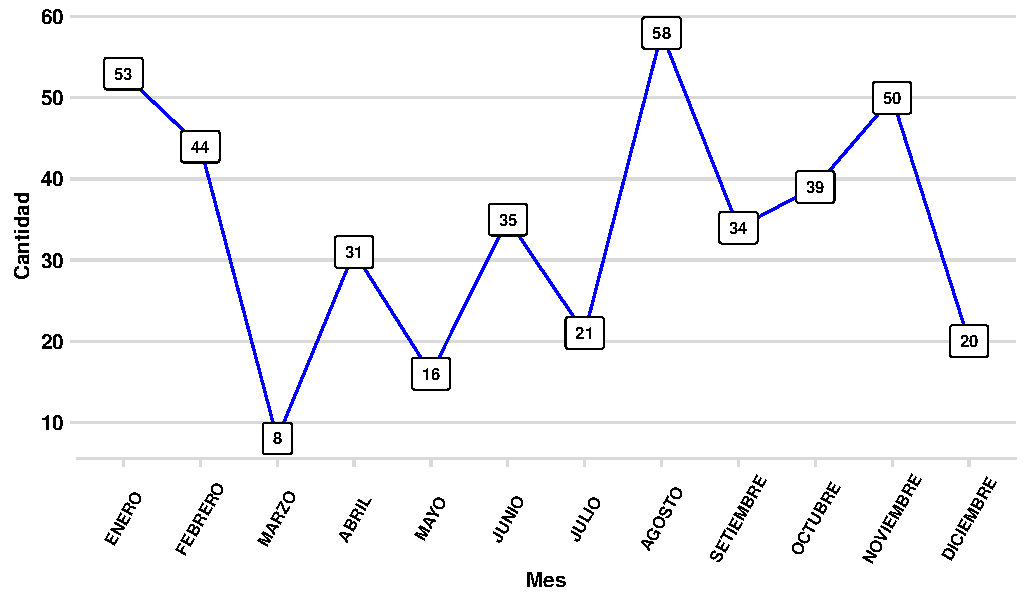
\includegraphics[width=15cm, height=5.95cm]{images/PROD001_demanda.pdf}}
  \label{fig:PROD001_demanda}
\end{figure}
La Figura \ref{fig:PROD001_demanda} muestra el diagrama de lineas que representa la evolución de la demanda del paquete de tratamiento talla ``S'' por mes en el año 2024, se observa que la demanda tiene un comportamiento determinístico a través de los meses del año, a excepción del mes de marzo y agosto donde hubo puntos extremos, asimismo no se observa una tendencia y solo estacionariedad en el tiempo, por lo que tomando estos casos y el comportamiento de la demanda es necesario utilizar un \textsl{modelo determinístico EOQ}.

Tomando en cuenta la demanda total anual de la Tabla \ref{table:GrupoA_Area}, el costo de compra de la Tabla \ref{table:GrupoA_Costo_Compra}, el costo de preparación estimado de la Tabla \ref{table:GrupoA_Costo_Preparacion}, el costo de retención estimado de la Tabla \ref{table:GrupoA_Costo_Retencion} y tiempo de reabastecimiento del pedido brindado por el área de logística se tienen los siguientes valores:
\begin{itemize}
    \item \textbf{Demanda ($D$):} 409 unidades
    \item \textbf{Costo de compra ($C$):} S/ 4,282.68 por unidad
    \item \textbf{Costo de preparación ($K$):} S/ 3.80
    \item \textbf{Costo de retención ($h$):} S/ 9.90
    \item \textbf{Tiempo de entrega ($L$):} 7 días
\end{itemize}
Hallamos la cantidad de pedido óptima $y^*$ mediante la expresión (\ref{yopt}) de la siguiente manera
\begin{eqnarray}
    y^* &=& \sqrt{\frac{2KD}{h}} \nonumber \\
    y^* &=& \sqrt{\frac{2(3.8)(409)}{9.90}} \nonumber \\
    y^* &=& 17.72 \nonumber \\
    y^* &\thickapprox& 18 \text{ unidades} \nonumber
\end{eqnarray}
De la misma forma hallemos el intervalo de pedido óptimo $T^*$ utilizando la expresión (\ref{Topt}) 
\begin{eqnarray}
    T^* &=& \sqrt{\frac{2K}{Dh}} \nonumber \\
    T^* &=& \sqrt{\frac{2(3.8)}{(409)(9.9)}} \nonumber \\
    T^* &=& 0.0433 \nonumber
\end{eqnarray}
Asimismo tomemos la demanda por día laborable (52 semanas * 5 días/semana = 260 días laborables) de tal forma que vemos el momento de cuando pedir
\begin{eqnarray}
    T^* &=& 0.0433 (260 \text{ días laborables}) \nonumber \\   
    T^* &=& 11.26 \nonumber \\
    T^* &\thickapprox& 11 \text{ días laborables} \nonumber
\end{eqnarray}
Ahora hallemos el costo mínimo total de inventario óptimo $CTI(y^*)$ usando la expresión (\ref{CTIopt}).
\begin{eqnarray}
    CTI(y^*) &=& \sqrt{2hKD} + DC \nonumber \\
    CTI(y^*) &=& \sqrt{2(9.9)(3.8)(409)} + (409)(4282.68) \nonumber \\
    CTI(y^*) &=& \text{S/ 1,751,791.54} \nonumber
\end{eqnarray}
Por último hallemos el punto de reorden en base a la cantidad de pedido óptima y el tiempo de reabastecimiento de 7 días.
\begin{eqnarray}
    R &=& L_e D \nonumber \\
    R &=& (7) \left(\frac{409}{260 \text{ días laborables}} \right) \nonumber \\
    R &=& 11.01 \nonumber \\
    R &\thickapprox& 11 \text{ unidades} \nonumber
\end{eqnarray}
Esto quiere decir que cuando el inventario del producto llegue a 11 unidades se deben de realizar el pedido de 18 unidades, del cual el tiempo de pedido debería ser cada 11 días laborables teniendo un costo total de S/ 1,751,791.54
\subsubsection{KIT para procedimiento quirúrgico oftálmico (pack centurion ultra balance)}
El producto KIT para procedimiento quirúrgico oftálmico (pack centurion ultra balance) de FACO del área de oftalmología es utilizado para las cirugía de facoemulsificación para la extracción de la catarata, observemos la tendencia de la demanda a lo largo del año 2024.
\clearpage
\begin{figure}[H]
  \caption{Evolución demanda: KIT para procedimiento quirúrgico oftálmico (pack centurion ultra balance) de FACO - oftalmología}
  {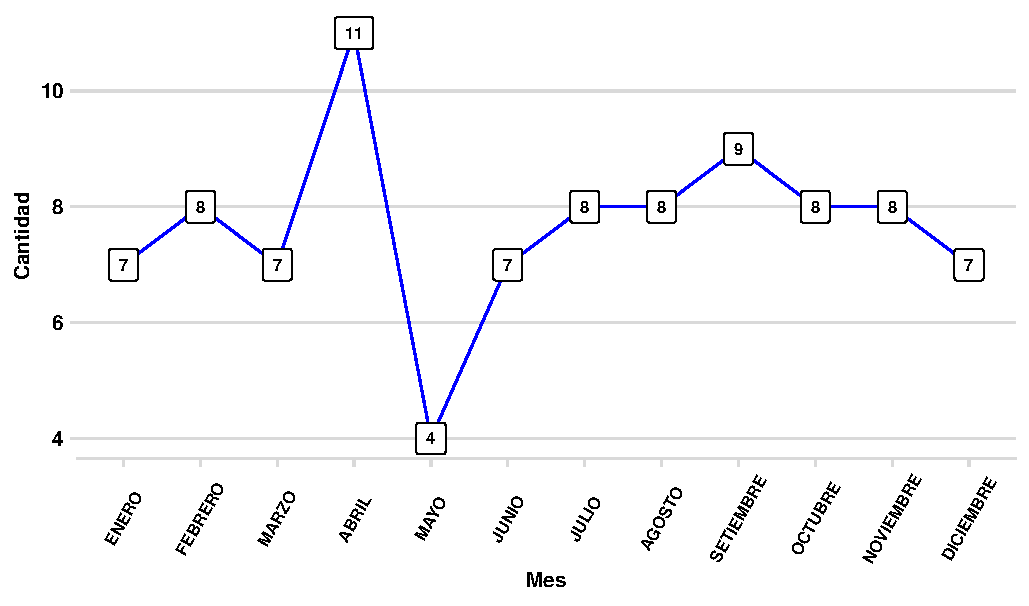
\includegraphics[width=15cm, height=5.95cm]{images/PROD002_demanda.pdf}}
  \label{fig:PROD002_demanda}
\end{figure}
La Figura \ref{fig:PROD002_demanda} muestra el diagrama de lineas que representa la evolución de la demanda del KIT para procedimiento quirúrgico oftálmico por mes en el año 2024, se observa que la demanda tiene un comportamiento determinístico a través de los meses del año, a excepción del mes de abril y mayo donde hubo puntos extremos, asimismo no se observa una tendencia y solo estacionariedad en el tiempo, por lo que tomando estos casos y el comportamiento de la demanda es necesario utilizar un \textsl{modelo determinístico EOQ}.

Tomando en cuenta la demanda total anual de la Tabla \ref{table:GrupoA_Area}, el costo de compra de la Tabla \ref{table:GrupoA_Costo_Compra}, el costo de preparación estimado de la Tabla \ref{table:GrupoA_Costo_Preparacion}, el costo de retención estimado de la Tabla \ref{table:GrupoA_Costo_Retencion} y tiempo de reabastecimiento del pedido brindado por el área de logística se tienen los siguientes valores:

\begin{itemize}
    \item \textbf{Demanda ($D$):} 92 unidades
    \item \textbf{Costo de compra ($C$):} S/ 542.60 por unidad
    \item \textbf{Costo de preparación ($K$):} S/ 17.31
    \item \textbf{Costo de retención ($h$):} S/ 13.64
    \item \textbf{Tiempo de entrega ($L$):} 3 días
\end{itemize}

Hallamos la cantidad de pedido óptima $y^*$ mediante la expresión (\ref{yopt}) de la siguiente manera
\begin{eqnarray}
    y^* &=& \sqrt{\frac{2KD}{h}} \nonumber \\
    y^* &=& \sqrt{\frac{2(17.31)(92)}{13.64}} \nonumber \\
    y^* &=& 15.28 \nonumber \\
    y^* &\thickapprox& 15 \text{ unidades} \nonumber
\end{eqnarray}
De la misma forma hallemos el intervalo de pedido óptimo $T^*$ utilizando la expresión (\ref{Topt}) 
\begin{eqnarray}
    T^* &=& \sqrt{\frac{2K}{Dh}} \nonumber \\
    T^* &=& \sqrt{\frac{2(17.31)}{(92)(13.64)}} \nonumber \\
    T^* &=& 0.1661 \nonumber
\end{eqnarray}
Asimismo tomemos la demanda por día laborable (52 semanas * 5 días/semana = 260 días laborables) de tal forma que vemos el momento de cuando pedir
\begin{eqnarray}
    T^* &=& 0.1661 (260 \text{ días laborables}) \nonumber \\   
    T^* &=& 43.19 \nonumber \\
    T^* &\thickapprox& 43 \text{ días laborables} \nonumber
\end{eqnarray}
Ahora hallemos el costo mínimo total de inventario óptimo $CTI(y^*)$ usando la expresión (\ref{CTIopt}).
\begin{eqnarray}
    CTI(y^*) &=& \sqrt{2hKD} + DC \nonumber \\
    CTI(y^*) &=& \sqrt{2(13.64)(17.31)(92)} + (92)(542.60) \nonumber \\
    CTI(y^*) &=& \text{S/ 50,127.63} \nonumber
\end{eqnarray}
Por último hallemos el punto de reorden en base a la cantidad de pedido óptima y el tiempo de reabastecimiento de 3 días.

\begin{eqnarray}
    R &=& L_e D \nonumber \\
  R &=& (3) \left(\frac{92}{260\text{ días laborables }} \right) \nonumber \\
  R &=& 1.06 \nonumber \\
  R &\thickapprox& 1\text{ unidad}
\end{eqnarray}

Esto quiere decir que cuando el inventario del producto llegue a 1 unidad se deben de realizar el pedido de 15 unidades, del cual el tiempo de pedido debería ser cada 43 días laborables teniendo un costo total de S/ 50,127.63
\subsubsection{Bolsa de solución BSS BAG 500 ml}

El producto bolsa de solución BSS BAG 500 ml de FACO del área de oftalmología es utilizado para las cirugía de facoemulsificación para la extracción de la catarata, primeramente observemos la tendencia de la demanda a lo largo del año 2024 en el siguiente gráfico.

\begin{figure}[H]
  \caption{Evolución demanda: Bolsa de solución BSS BAG 500 ml de FACO - oftalmología}
  {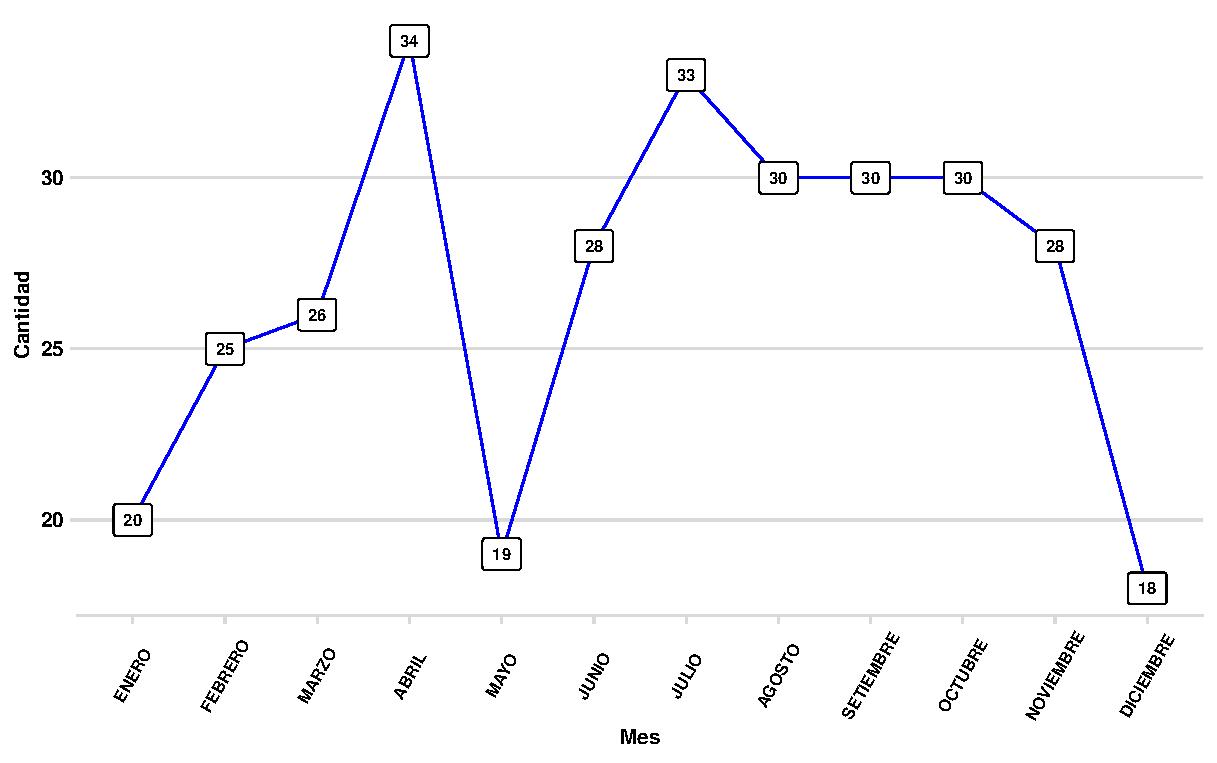
\includegraphics[width=15cm, height=5.95cm]{images/PROD003_demanda.pdf}}
  \label{fig:PROD003_demanda}
\end{figure}

La Figura \ref{fig:PROD003_demanda} muestra el diagrama de lineas que representa la evolución de la demanda de la bolsa de solución BSS BAG 500 ml por mes en el año 2024, se observa que la demanda tiene un comportamiento determinístico a través de los meses del año, a excepción del mes de enero, mayo y diciembre en donde hubo puntos extremos, asimismo no se observa una tendencia y solo estacionariedad en el tiempo, por lo que tomando estos casos y el comportamiento de la demanda es necesario utilizar un \textsl{modelo determinístico EOQ}.

Tomando en cuenta la demanda total anual de la Tabla \ref{table:GrupoA_Area}, el costo de compra de la Tabla \ref{table:GrupoA_Costo_Compra}, el costo de preparación estimado de la Tabla \ref{table:GrupoA_Costo_Preparacion}, el costo de retención estimado de la Tabla \ref{table:GrupoA_Costo_Retencion} y tiempo de reabastecimiento del pedido brindado por el área de logística se tienen los siguientes valores:

\begin{itemize}
    \item \textbf{Demanda ($D$):} 321 unidades
    \item \textbf{Costo de compra ($C$):} S/ 345.15 por unidad
    \item \textbf{Costo de preparación ($K$):} S/ 19.21
    \item \textbf{Costo de retención ($h$):} S/ 29.42
    \item \textbf{Tiempo de entrega ($L$):} 3 días
\end{itemize}

Hallamos la cantidad de pedido óptima $y^*$ mediante la expresión (\ref{yopt}) de la siguiente manera
\begin{eqnarray}
    y^* &=& \sqrt{\frac{2KD}{h}} \nonumber \\
    y^* &=& \sqrt{\frac{2(19.21)(321)}{29.42}} \nonumber \\
    y^* &=& 20.47 \nonumber \\
    y^* &\thickapprox& 20 \text{ unidades} \nonumber
\end{eqnarray}
De la misma forma hallemos el intervalo de pedido óptimo $T^*$ utilizando la expresión (\ref{Topt}) 
\begin{eqnarray}
    T^* &=& \sqrt{\frac{2K}{Dh}} \nonumber \\
    T^* &=& \sqrt{\frac{2(19.21)}{(321)(29.42)}} \nonumber \\
    T^* &=& 0.0638 \nonumber
\end{eqnarray}
Asimismo tomemos la demanda por día laborable (52 semanas * 5 días/semana = 260 días laborables) de tal forma que vemos el momento de cuando pedir

\begin{eqnarray}
    T^* &=& 0.0638 (260 \text{ días laborables}) \nonumber \\   
    T^* &=& 16.58 \nonumber \\
    T^* &\thickapprox& 17 \text{ días laborables} \nonumber
\end{eqnarray}
Ahora hallemos el costo mínimo total de inventario óptimo $CTI(y^*)$ usando la expresión (\ref{CTIopt}).
\begin{eqnarray}
    CTI(y^*) &=& \sqrt{2hKD} + DC \nonumber \\
    CTI(y^*) &=& \sqrt{2(29.42)(19.21)(321)} + (321)(345.15) \nonumber \\
    CTI(y^*) &=& \text{S/ 111,395.51} \nonumber
\end{eqnarray}
Por último hallemos el punto de reorden en base a la cantidad de pedido óptima y el tiempo de reabastecimiento de 3 días.
\begin{eqnarray}
    R &=& L_e D \nonumber \\
    R &=& (3) \left(\frac{321}{260 \text{ días laborables}} \right) \nonumber \\
    R &=& 3.70 \nonumber \\
    R &\thickapprox& 4 \text{ unidades} \nonumber
\end{eqnarray}

Esto quiere decir que cuando el inventario del producto llegue a 4 unidades se deben de realizar el pedido de 20 unidades, del cual el tiempo de pedido debería ser cada 17 días laborables teniendo un costo total de S/ 111,395.51
\subsubsection{Cuchillo de hendidura CLEAR CUT HP2 2.4 mm bisel doble, intrepido sistema microcoaxial}

El producto cuchillo de hendidura CLEAR CUT HP2 2.4 mm bisel doble, intrepido sistema microcoaxial de FACO del área de oftalmología es utilizado para las cirugía de facoemulsificación y extracción manual de catarata con incisión pequeña que son las cirugías para la extracción de la catarata, primeramente observemos la tendencia de la demanda a lo largo del año 2024 en el siguiente gráfico.

\begin{figure}[H]
  \caption{Evolución demanda: Cuchillo de hendidura CLEAR CUT HP2 2.4 mm bisel doble, intrepido sistema microcoaxial de FACO - oftalmología}
  {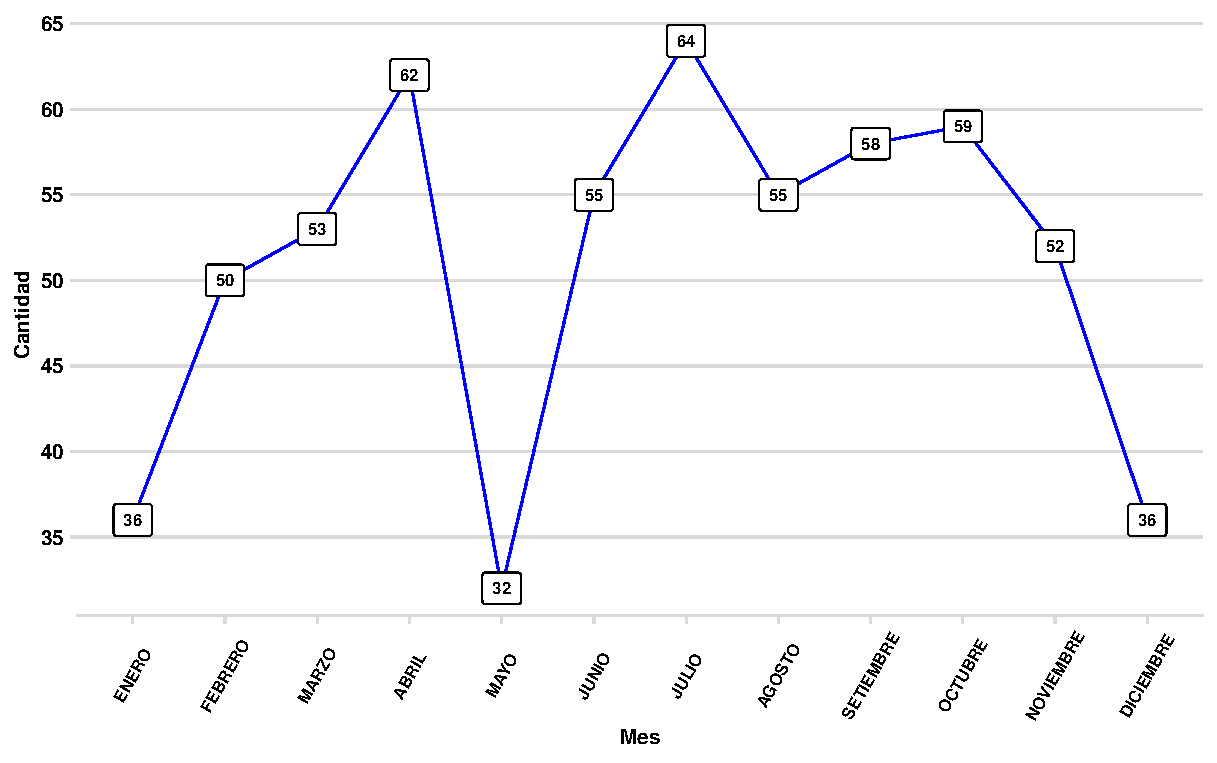
\includegraphics[width=15cm, height=5.95cm]{images/PROD004_demanda.pdf}}
  \label{fig:PROD004_demanda}
\end{figure}

La Figura \ref{fig:PROD004_demanda} muestra el diagrama de lineas que representa la evolución de la demanda del cuchillo de hendidura CLEAR CUT HP2 2.4 mm bisel doble, intrepido sistema microcoaxial por mes en el año 2024, se observa que la demanda tiene un comportamiento determinístico a través de los meses del año, a excepción del mes de enero, mayo y diciembre en donde hubo puntos extremos, asimismo no se observa una tendencia y solo estacionariedad en el tiempo, por lo que tomando estos casos y el comportamiento de la demanda es necesario utilizar un \textsl{modelo determinístico EOQ}.

Tomando en cuenta la demanda total anual de la Tabla \ref{table:GrupoA_Area}, el costo de compra de la Tabla \ref{table:GrupoA_Costo_Compra}, el costo de preparación estimado de la Tabla \ref{table:GrupoA_Costo_Preparacion}, el costo de retención estimado de la Tabla \ref{table:GrupoA_Costo_Retencion} y tiempo de reabastecimiento del pedido brindado por el área de logística se tienen los siguientes valores:

\begin{itemize}
    \item \textbf{Demanda ($D$):} 612 unidades
    \item \textbf{Costo de compra ($C$):} S/ 69.80 por unidad
    \item \textbf{Costo de preparación ($K$):} S/ 9.61
    \item \textbf{Costo de retención ($h$):} S/ 6.15
\end{itemize}
\begin{itemize}
  \item \textbf{Tiempo de entrega ($L$):} 3 días
\end{itemize}

Hallamos la cantidad de pedido óptima $y^*$ mediante la expresión (\ref{yopt}) de la siguiente manera
\begin{eqnarray}
    y^* &=& \sqrt{\frac{2KD}{h}} \nonumber \\
    y^* &=& \sqrt{\frac{2(9.61)(612)}{6.15}} \nonumber \\
    y^* &=& 43.73 \nonumber \\
    y^* &\thickapprox& 44 \text{ unidades} \nonumber
\end{eqnarray}
De la misma forma hallemos el intervalo de pedido óptimo $T^*$ utilizando la expresión (\ref{Topt}) 
\begin{eqnarray}
    T^* &=& \sqrt{\frac{2K}{Dh}} \nonumber \\
    T^* &=& \sqrt{\frac{2(9.61)}{(612)(6.15)}} \nonumber \\
    T^* &=& 0.0715 \nonumber
\end{eqnarray}
Asimismo tomemos la demanda por día laborable (52 semanas * 5 días/semana = 260 días laborables) de tal forma que vemos el momento de cuando pedir
\begin{eqnarray}
    T^* &=& 0.0715 (260 \text{ días laborables}) \nonumber \\   
    T^* &=& 18.58 \nonumber \\
    T^* &\thickapprox& 19 \text{ días laborables} \nonumber
\end{eqnarray}
Ahora hallemos el costo mínimo total de inventario óptimo $CTI(y^*)$ usando la expresión (\ref{CTIopt}).
\begin{eqnarray}
    CTI(y^*) &=& \sqrt{2hKD} + DC \nonumber \\
    CTI(y^*) &=& \sqrt{2(6.15)(9.61)(612)} + (612)(69.80) \nonumber \\
    CTI(y^*) &=& \text{S/ 42,986.56} \nonumber
\end{eqnarray}
\clearpage
\noindent Por último hallemos el punto de reorden en base a la cantidad de pedido óptima y el tiempo de reabastecimiento de 3 días.
\begin{eqnarray}
    R &=& L_e D \nonumber \\
    R &=& (3) \left(\frac{612}{260 \text{ días laborables}} \right) \nonumber \\
    R &=& 7.06 \nonumber \\
    R &\thickapprox& 7 \text{ unidades} \nonumber
\end{eqnarray}

Esto quiere decir que cuando el inventario del producto llegue a 7 unidades se deben de realizar el pedido de 44 unidades, del cual el tiempo de pedido debería ser cada 19 días laborables teniendo un costo total de S/ 42,986.56
\subsubsection{AJL VISC 1.4$\%$ - pack solución viscoelástica para uso intraocular hialuronato sódico 14 mg/ml canula 1x27g}

El producto AJL VISC 1.4$\%$ - pack solución viscoelástica para uso intraocular de FACO del área de oftalmología es utilizado para las cirugía de facoemulsificación, extracción manual de catarata con incisión pequeña para la extracción de catarata y cirugía de válvula, primeramente observemos la tendencia de la demanda a lo largo del año 2024 en el siguiente gráfico.

\begin{figure}[H]
  \caption{Evolución demanda: AJL VISC 1.4$\%$ - pack solución viscoelástica para uso intraocular de FACO - oftalmología}
  {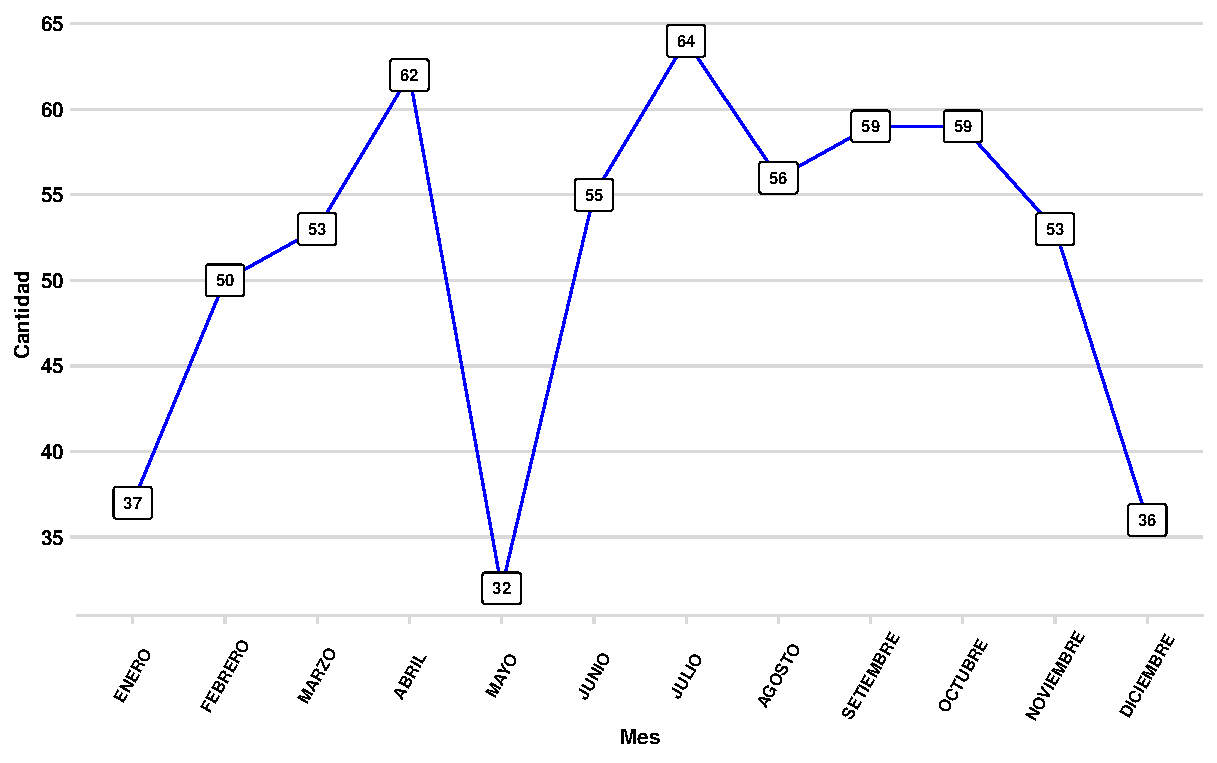
\includegraphics[width=15cm, height=5.95cm]{images/PROD005_demanda.pdf}}
  \label{fig:PROD005_demanda}
\end{figure}

La Figura \ref{fig:PROD005_demanda} muestra el diagrama de lineas que representa la evolución de la demanda de AJL VISC 1.4$\%$ - pack solución viscoelástica para uso intraocular hialuronato sódico 14 mg/ml canula 1x27g por mes en el año 2024, se observa que la demanda tiene un comportamiento determinístico a través de los meses del año, a excepción del mes de enero, mayo y diciembre en donde hubo puntos extremos, asimismo no se observa una tendencia y solo estacionariedad en el tiempo, por lo que tomando estos casos y el comportamiento de la demanda es necesario utilizar un \textsl{modelo determinístico EOQ}.

Tomando en cuenta la demanda total anual de la Tabla \ref{table:GrupoA_Area}, el costo de compra de la Tabla \ref{table:GrupoA_Costo_Compra}, el costo de preparación estimado de la Tabla \ref{table:GrupoA_Costo_Preparacion}, el costo de retención estimado de la Tabla \ref{table:GrupoA_Costo_Retencion} y tiempo de reabastecimiento del pedido brindado por el área de logística se tienen los siguientes valores:

\begin{itemize}
    \item \textbf{Demanda ($D$):} 616 unidades
    \item \textbf{Costo de compra ($C$):} S/ 90.00 por unidad
    \item \textbf{Costo de preparación ($K$):} S/ 7.70
    \item \textbf{Costo de retención ($h$):} S/ 11.23
    \item \textbf{Tiempo de entrega ($L$):} 7 días
\end{itemize}

Hallamos la cantidad de pedido óptima $y^*$ mediante la expresión (\ref{yopt}) de la siguiente manera
\begin{eqnarray}
    y^* &=& \sqrt{\frac{2KD}{h}} \nonumber \\
    y^* &=& \sqrt{\frac{2(7.7)(616)}{11.23}} \nonumber \\
    y^* &=& 29.06 \nonumber \\
    y^* &\thickapprox& 29 \text{ unidades} \nonumber
\end{eqnarray}
De la misma forma hallemos el intervalo de pedido óptimo $T^*$ utilizando la expresión (\ref{Topt}) 
\begin{eqnarray}
    T^* &=& \sqrt{\frac{2K}{Dh}} \nonumber
\end{eqnarray}
\begin{eqnarray}
    T^* &=& \sqrt{\frac{2(7.7)}{(616)(11.23)}} \nonumber \\
    T^* &=& 0.0472 \nonumber
\end{eqnarray}
Asimismo tomemos la demanda por día laborable (52 semanas * 5 días/semana = 260 días laborables) de tal forma que vemos el momento de cuando pedir
\begin{eqnarray}
    T^* &=& 0.0472 (260 \text{ días laborables}) \nonumber \\   
    T^* &=& 12.27 \nonumber \\
    T^* &\thickapprox& 12 \text{ días laborables} \nonumber
\end{eqnarray}
Ahora hallemos el costo mínimo total de inventario óptimo $CTI(y^*)$ usando la expresión (\ref{CTIopt}).
\begin{eqnarray}
    CTI(y^*) &=& \sqrt{2hKD} + DC \nonumber \\
    CTI(y^*) &=& \sqrt{2(11.23)(7.7)(616)} + (616)(90) \nonumber \\
    CTI(y^*) &=& \text{S/ 55,766.39} \nonumber
\end{eqnarray}
Por último hallemos el punto de reorden en base a la cantidad de pedido óptima y el tiempo de reabastecimiento de 7 días.
\begin{eqnarray}
    R &=& L_e D \nonumber \\
    R &=& (7) \left(\frac{616}{260 \text{ días laborables}} \right) \nonumber \\
    R &=& 16.58 \nonumber \\
    R &\thickapprox& 17 \text{ unidades} \nonumber
\end{eqnarray}

Esto quiere decir que cuando el inventario del producto llegue a 17 unidades se deben de realizar el pedido de 29 unidades, del cual el tiempo de pedido debería ser cada 12 días laborables teniendo un costo total de S/ 55,766.39
\clearpage
\subsubsection{Cuchillo lateral CLEAR CUT doble bisel 1.2 mm angulado}

El producto cuchillo lateral CLEAR CUT doble bisel 1.2 mm angulado de insumos generales del área de oftalmología es utilizado para las cirugía de facoemulsificación y extracción manual de catarata con incisión pequeña que son las cirugías para la extracción de catarata, primeramente observemos la tendencia de la demanda a lo largo del año 2024 en el siguiente gráfico.

\begin{figure}[H]
  \caption{Evolución demanda: Cuchillo lateral CLEAR CUT doble bisel 1.2 mm angulado de insumos generales - oftalmología}
  {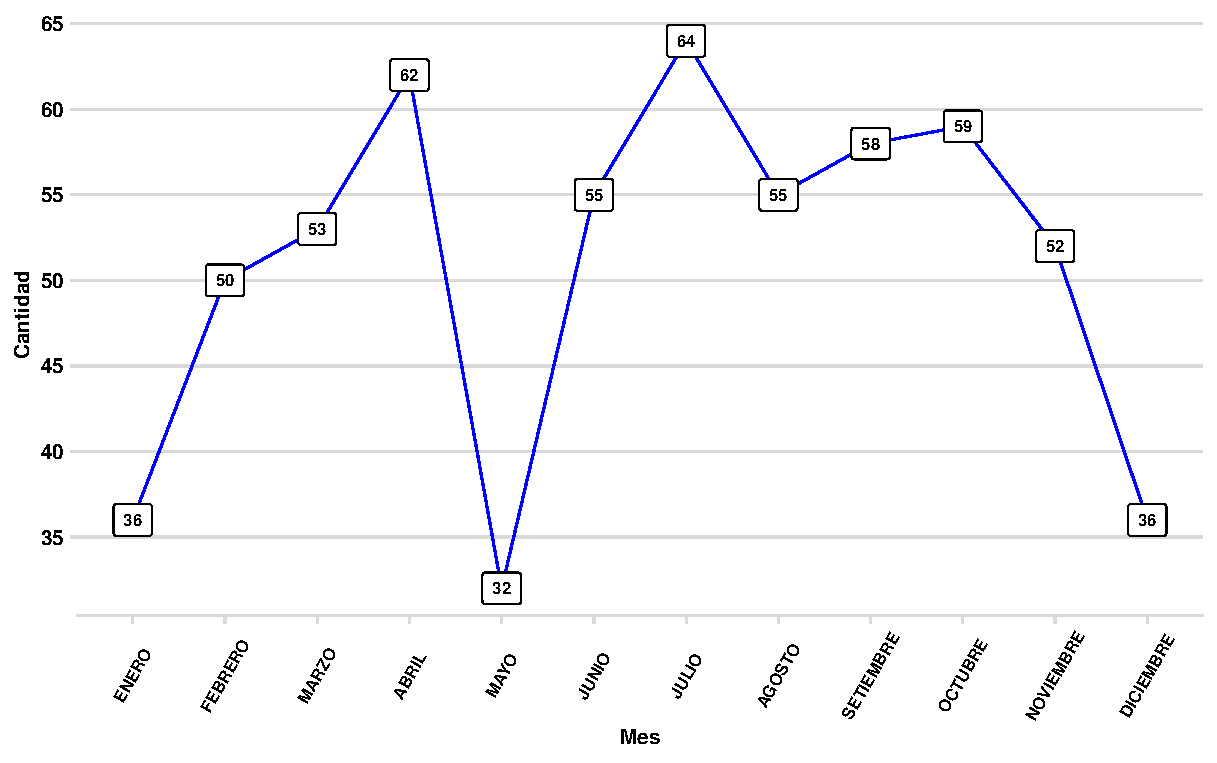
\includegraphics[width=15cm, height=5.95cm]{images/PROD006_demanda.pdf}}
  \label{fig:PROD006_demanda}
\end{figure}

La Figura \ref{fig:PROD006_demanda} muestra el diagrama de lineas que representa la evolución de la demanda del cuchillo lateral CLEAR CUT doble bisel 1.2 mm angulado por mes en el año 2024, se observa que la demanda tiene un comportamiento determinístico a través de los meses del año, a excepción del mes de enero, mayo y diciembre en donde hubo puntos extremos, asimismo no se observa una tendencia y solo estacionariedad en el tiempo, por lo que tomando estos casos y el comportamiento de la demanda es necesario utilizar un \textsl{modelo determinístico EOQ}.

Tomando en cuenta la demanda total anual de la Tabla \ref{table:GrupoA_Area}, el costo de compra de la Tabla \ref{table:GrupoA_Costo_Compra}, el costo de preparación estimado de la Tabla \ref{table:GrupoA_Costo_Preparacion}, el costo de retención estimado de la Tabla \ref{table:GrupoA_Costo_Retencion} y tiempo de reabastecimiento del pedido brindado por el área de logística se tienen los siguientes valores:

\begin{itemize}
    \item \textbf{Demanda ($D$):} 612 unidades
    \item \textbf{Costo de compra ($C$):} S/ 72.81 por unidad
    \item \textbf{Costo de preparación ($K$):} S/ 3.80
    \item \textbf{Costo de retención ($h$):} S/ 11.50
    \item \textbf{Tiempo de entrega ($L$):} 3 días
\end{itemize}

Hallamos la cantidad de pedido óptima $y^*$ mediante la expresión (\ref{yopt}) de la siguiente manera
\begin{eqnarray}
    y^* &=& \sqrt{\frac{2KD}{h}} \nonumber \\
    y^* &=& \sqrt{\frac{2(3.8)(612)}{11.5}} \nonumber \\
    y^* &=& 20.11 \nonumber \\
    y^* &\thickapprox& 20 \text{ unidades} \nonumber
\end{eqnarray}
De la misma forma hallemos el intervalo de pedido óptimo $T^*$ utilizando la expresión (\ref{Topt}) 
\begin{eqnarray}
    T^* &=& \sqrt{\frac{2K}{Dh}} \nonumber \\
    T^* &=& \sqrt{\frac{2(3.8)}{(612)(11.5)}} \nonumber \\
    T^* &=& 0.0329 \nonumber
\end{eqnarray}
Asimismo tomemos la demanda por día laborable (52 semanas * 5 días/semana = 260 días laborables) de tal forma que vemos el momento de cuando pedir
\begin{eqnarray}
    T^* &=& 0.0329 (260 \text{ días laborables}) \nonumber \\   
    T^* &=& 8.54 \nonumber \\
    T^* &\thickapprox& 9 \text{ días laborables} \nonumber
\end{eqnarray}
Ahora hallemos el costo mínimo total de inventario óptimo $CTI(y^*)$ usando la expresión (\ref{CTIopt}).
\begin{eqnarray}
    CTI(y^*) &=& \sqrt{2hKD} + DC \nonumber
\end{eqnarray}
\begin{eqnarray}
    CTI(y^*) &=& \sqrt{2(11.5)(3.8)(612)} + (612)(72.81) \nonumber \\
    CTI(y^*) &=& \text{S/ 44,791.00} \nonumber
\end{eqnarray}
Por último hallemos el punto de reorden en base a la cantidad de pedido óptima y el tiempo de reabastecimiento de 3 días.
\begin{eqnarray}
    R &=& L_e D \nonumber \\
    R &=& (3) \left(\frac{612}{260 \text{ días laborables}} \right) \nonumber \\
    R &=& 7.06 \nonumber \\
    R &\thickapprox& 7 \text{ unidades} \nonumber
\end{eqnarray}

Esto quiere decir que cuando el inventario del producto llegue a 7 unidades se deben de realizar el pedido de 20 unidades, del cual el tiempo de pedido debería ser cada 9 días laborables teniendo un costo total de S/ 44,791.00
\subsubsection{Solución de riboflavina VIBEX RAPID 0.1$\%$ isotonico jeringa de 1.5 ml}

El producto solución de riboflavina VIBEX RAPID 0.1$\%$ isotonico jeringa de 1.5 ml de CROSSLINKING del área de oftalmología es utilizado para las cirugías de queratocono, primeramente observemos la tendencia de la demanda a lo largo del año 2024 en el siguiente gráfico.

\begin{figure}[H]
  \caption{Evolución demanda: Solución de riboflavina VIBEX RAPID 0.1$\%$ de CROSSLINKING - oftalmología}
  {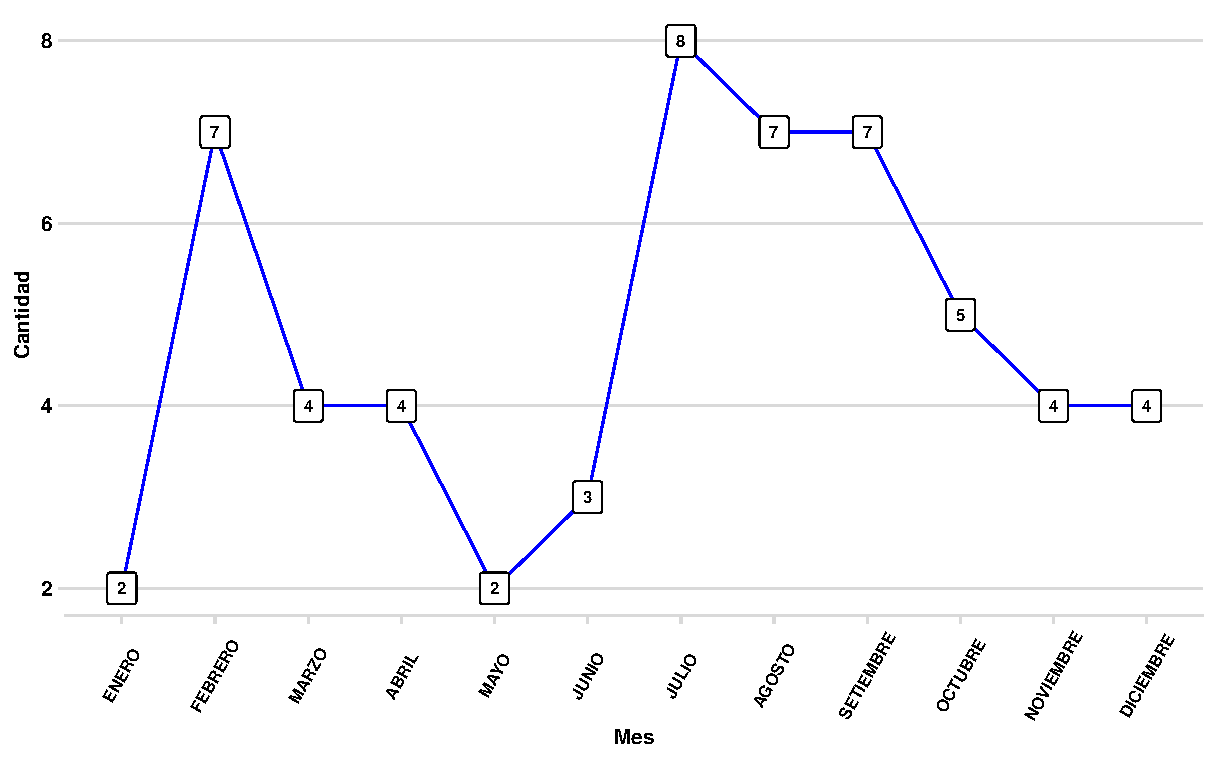
\includegraphics[width=15cm, height=5.85cm]{images/PROD007_demanda.pdf}}
  \label{fig:PROD007_demanda}
\end{figure}

La Figura \ref{fig:PROD007_demanda} muestra el diagrama de lineas que representa la evolución de la demanda de la solución de riboflavina VIBEX RAPID 0.1$\%$ por mes en el año 2024, se observa que la demanda tiene un comportamiento determinístico y estacionario sin tendencia a través de los meses del año, por lo que tomando estos casos y el comportamiento de la demanda es necesario utilizar un \textsl{modelo determinístico EOQ}.

Tomando en cuenta la demanda total anual de la Tabla \ref{table:GrupoA_Area}, el costo de compra de la Tabla \ref{table:GrupoA_Costo_Compra}, el costo de preparación estimado de la Tabla \ref{table:GrupoA_Costo_Preparacion}, el costo de retención estimado de la Tabla \ref{table:GrupoA_Costo_Retencion} y tiempo de reabastecimiento del pedido brindado por el área de logística se tienen los siguientes valores:

\begin{itemize}
    \item \textbf{Demanda ($D$):} 57 unidades
    \item \textbf{Costo de compra ($C$):} S/ 362.94 por unidad
    \item \textbf{Costo de preparación ($K$):} S/ 1.90
    \item \textbf{Costo de retención ($h$):} S/ 6.42
    \item \textbf{Tiempo de entrega ($L$):} 7 días
\end{itemize}

Hallamos la cantidad de pedido óptima $y^*$ mediante la expresión (\ref{yopt}) de la siguiente manera
\begin{eqnarray}
    y^* &=& \sqrt{\frac{2KD}{h}} \nonumber \\
    y^* &=& \sqrt{\frac{2(1.9)(57)}{6.42}} \nonumber \\
    y^* &=& 5.81 \nonumber \\
    y^* &\thickapprox& 6 \text{ unidades} \nonumber
\end{eqnarray}
De la misma forma hallemos el intervalo de pedido óptimo $T^*$ utilizando la expresión (\ref{Topt}) 
\begin{eqnarray}
    T^* &=& \sqrt{\frac{2K}{Dh}} \nonumber \\
    T^* &=& \sqrt{\frac{2(1.9)}{(57)(6.42)}} \nonumber \\
    T^* &=& 0.1019 \nonumber
\end{eqnarray}
Asimismo tomemos la demanda por día laborable (52 semanas * 5 días/semana = 260 días laborables) de tal forma que vemos el momento de cuando pedir
\begin{eqnarray}
    T^* &=& 0.1019 (260 \text{ días laborables}) \nonumber \\   
    T^* &=& 26.49 \nonumber \\
    T^* &\thickapprox& 26 \text{ días laborables} \nonumber
\end{eqnarray}
Ahora hallemos el costo mínimo total de inventario óptimo $CTI(y^*)$ usando la expresión (\ref{CTIopt}).
\begin{eqnarray}
    CTI(y^*) &=& \sqrt{2hKD} + DC \nonumber \\
    CTI(y^*) &=& \sqrt{2(6.42)(1.9)(57)} + (57)(362.94) \nonumber \\
    CTI(y^*) &=& \text{S/ 20,724.87} \nonumber
\end{eqnarray}
Por último hallemos el punto de reorden en base a la cantidad de pedido óptima y el tiempo de reabastecimiento de 7 días.
\begin{eqnarray}
    R &=& L_e D \nonumber \\
    R &=& (7) \left(\frac{57}{260 \text{ días laborables}} \right) \nonumber \\
    R &=& 1.53 \nonumber \\
    R &\thickapprox& 2 \text{ unidades} \nonumber
\end{eqnarray}

Esto quiere decir que cuando el inventario del producto llegue a 2 unidades se deben de realizar el pedido de 6 unidades, del cual el tiempo de pedido debería ser cada 26 días laborables teniendo un costo total de S/ 20,724.87
\subsubsection{Anterior chamber cannula 27g x 9mm BEND}

El producto anterior chamber cannula 27g x 9mm BEND de INLASER del área de oftalmología es utilizado para las cirugías refractivas LASIK, Presbyond y retoques LASIK realizados, observemos la tendencia de la demanda a lo largo del año 2024 en el siguiente gráfico.

\begin{figure}[H]
  \caption{Evolución demanda: Anterior chamber cannula 27g x 9mm BEND de INLASER - oftalmología}
  {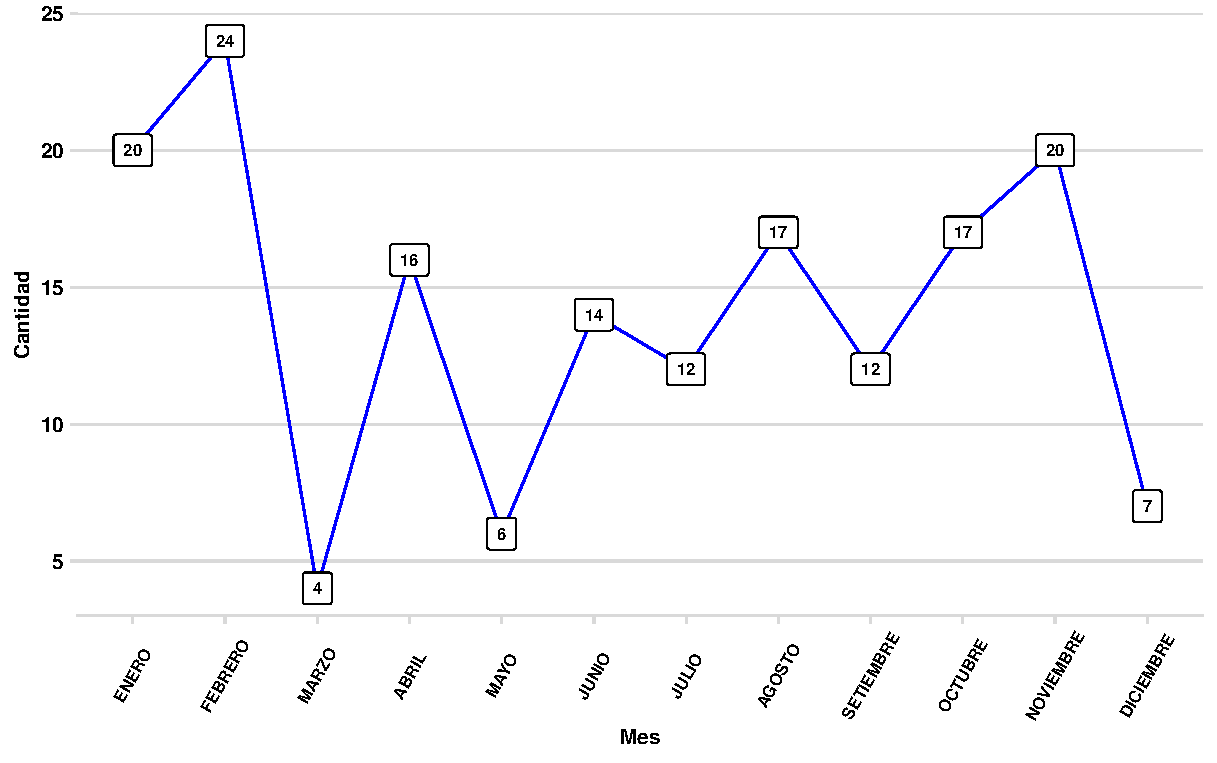
\includegraphics[width=15cm, height=5.95cm]{images/PROD008_demanda.pdf}}
  \label{fig:PROD008_demanda}
\end{figure}

La Figura \ref{fig:PROD008_demanda} muestra el diagrama de lineas que representa la evolución de la demanda del anterior chamber cannula 27g x 9mm BEND por mes en el año 2024, se observa que la demanda tiene un comportamiento determinístico y estacionario sin tendencia a través de los meses del año, por lo que tomando estos casos y el comportamiento de la demanda es necesario utilizar un \textsl{modelo determinístico EOQ}.

Tomando en cuenta la demanda total anual de la Tabla \ref{table:GrupoA_Area}, el costo de compra de la Tabla \ref{table:GrupoA_Costo_Compra}, el costo de preparación estimado de la Tabla \ref{table:GrupoA_Costo_Preparacion}, el costo de retención estimado de la Tabla \ref{table:GrupoA_Costo_Retencion} y tiempo de reabastecimiento del pedido brindado por el área de logística se tienen los siguientes valores:

\begin{itemize}
    \item \textbf{Demanda ($D$):} 169 unidades
    \item \textbf{Costo de compra ($C$):} S/ 16.00 por unidad
    \item \textbf{Costo de preparación ($K$):} S/ 7.70
    \item \textbf{Costo de retención ($h$):} S/ 12.30
    \item \textbf{Tiempo de entrega ($L$):} 7 días
\end{itemize}
Hallamos la cantidad de pedido óptima $y^*$ mediante la expresión (\ref{yopt}) de la siguiente manera
\begin{eqnarray}
    y^* &=& \sqrt{\frac{2KD}{h}} \nonumber
\end{eqnarray}
\begin{eqnarray}
    y^* &=& \sqrt{\frac{2(7.7)(169)}{12.3}} \nonumber \\
    y^* &=& 14.55 \nonumber \\
    y^* &\thickapprox& 15 \text{ unidades} \nonumber
\end{eqnarray}
De la misma forma hallemos el intervalo de pedido óptimo $T^*$ utilizando la expresión (\ref{Topt}) 
\begin{eqnarray}
    T^* &=& \sqrt{\frac{2K}{Dh}} \nonumber \\
    T^* &=& \sqrt{\frac{2(7.7)}{(169)(12.3)}} \nonumber \\
    T^* &=& 0.0861 \nonumber
\end{eqnarray}
Asimismo tomemos la demanda por día laborable (52 semanas * 5 días/semana = 260 días laborables) de tal forma que vemos el momento de cuando pedir
\begin{eqnarray}
    T^* &=& 0.0861 (260 \text{ días laborables}) \nonumber \\   
    T^* &=& 22.38 \nonumber \\
    T^* &\thickapprox& 22 \text{ días laborables} \nonumber
\end{eqnarray}
Ahora hallemos el costo mínimo total de inventario óptimo $CTI(y^*)$ usando la expresión (\ref{CTIopt}).
\begin{eqnarray}
    CTI(y^*) &=& \sqrt{2hKD} + DC \nonumber \\
    CTI(y^*) &=& \sqrt{2(12.3)(7.7)(169)} + (169)(16) \nonumber \\
    CTI(y^*) &=& \text{S/ 2,882.92} \nonumber
\end{eqnarray}
Por último hallemos el punto de reorden en base a la cantidad de pedido óptima y el tiempo de reabastecimiento de 7 días.
\begin{eqnarray}
    R &=& L_e D \nonumber \\
    R &=& (7) \left(\frac{169}{260 \text{ días laborables}} \right) \nonumber
\end{eqnarray}
\begin{eqnarray}
    R &=& 4.55 \nonumber \\
    R &\thickapprox& 5 \text{ unidades} \nonumber
\end{eqnarray}

Esto quiere decir que cuando el inventario del producto llegue a 5 unidades se deben de realizar el pedido de 15 unidades, del cual el tiempo de pedido debería ser cada 22 días laborables teniendo un costo total de S/ 2,882.92
\subsubsection{Canula para cistotoma formada 27g}

El producto canula para cistotoma formada 27g de FACO del área de oftalmología es utilizado para la cirugía de facoemulsificación y extracción manual de catarata con incisión pequeña que son las cirugías para la extracción de catarata, primeramente observemos la tendencia de la demanda a lo largo del año 2024 en el siguiente gráfico.

\begin{figure}[H]
  \caption{Evolución demanda: canula para cistotoma formada 27g de FACO - oftalmología}
  {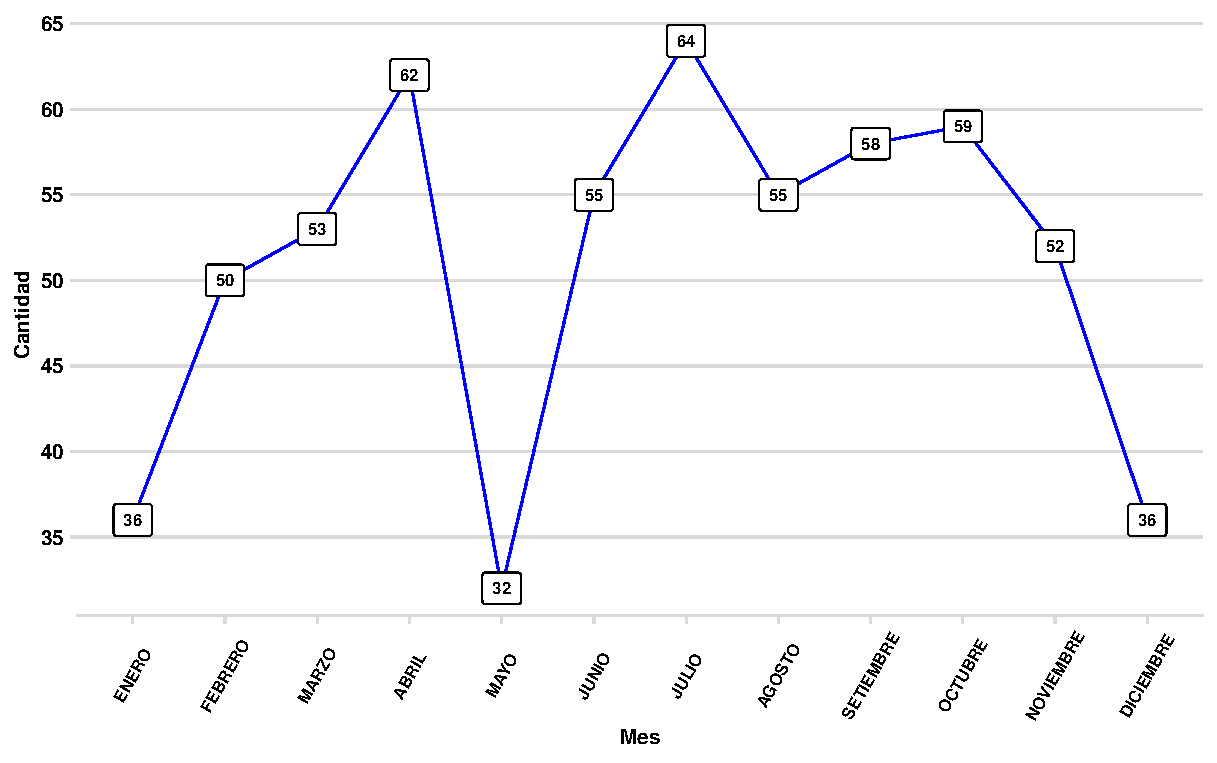
\includegraphics[width=15cm, height=5.95cm]{images/PROD009_demanda.pdf}}
  \label{fig:PROD009_demanda}
\end{figure}

La Figura \ref{fig:PROD009_demanda} muestra el diagrama de lineas que representa la evolución de la demanda de la canula para cistotoma formada 27g por mes en el año 2024, se observa que la demanda tiene un comportamiento determinístico y estacionario sin tendencia a través de los meses del año, por lo que tomando estos casos y el comportamiento de la demanda es necesario utilizar un \textsl{modelo determinístico EOQ}.

Tomando en cuenta la demanda total anual de la Tabla \ref{table:GrupoA_Area}, el costo de compra de la Tabla \ref{table:GrupoA_Costo_Compra}, el costo de preparación estimado de la Tabla \ref{table:GrupoA_Costo_Preparacion}, el costo de retención estimado de la Tabla \ref{table:GrupoA_Costo_Retencion} y tiempo de reabastecimiento del pedido brindado por el área de logística se tienen los siguientes valores:

\begin{itemize}
    \item \textbf{Demanda ($D$):} 612 unidades
    \item \textbf{Costo de compra ($C$):} S/ 143.00 por unidad
    \item \textbf{Costo de preparación ($K$):} S/ 9.61
    \item \textbf{Costo de retención ($h$):} S/ 8.56
    \item \textbf{Tiempo de entrega ($L$):} 7 días
\end{itemize}

Hallamos la cantidad de pedido óptima $y^*$ mediante la expresión (\ref{yopt}) de la siguiente manera
\begin{eqnarray}
    y^* &=& \sqrt{\frac{2KD}{h}} \nonumber \\
    y^* &=& \sqrt{\frac{2(9.61)(612)}{8.56}} \nonumber \\
    y^* &=& 37.07 \nonumber \\
    y^* &\thickapprox& 37 \text{ unidades} \nonumber
\end{eqnarray}
De la misma forma hallemos el intervalo de pedido óptimo $T^*$ utilizando la expresión (\ref{Topt}) 
\begin{eqnarray}
    T^* &=& \sqrt{\frac{2K}{Dh}} \nonumber \\
    T^* &=& \sqrt{\frac{2(9.61)}{(612)(8.56)}} \nonumber \\
    T^* &=& 0.0606 \nonumber
\end{eqnarray}
Asimismo tomemos la demanda por día laborable (52 semanas * 5 días/semana = 260 días laborables) de tal forma que vemos el momento de cuando pedir
\begin{eqnarray}
    T^* &=& 0.0606 (260 \text{ días laborables}) \nonumber \\   
    T^* &=& 15.75 \nonumber \\
    T^* &\thickapprox& 16 \text{ días laborables} \nonumber
\end{eqnarray}
Ahora hallemos el costo mínimo total de inventario óptimo $CTI(y^*)$ usando la expresión (\ref{CTIopt}).
\begin{eqnarray}
    CTI(y^*) &=& \sqrt{2hKD} + DC \nonumber \\
    CTI(y^*) &=& \sqrt{2(8.56)(9.61)(612)} + (612)(143) \nonumber \\
    CTI(y^*) &=& \text{S/ 87,833.31} \nonumber
\end{eqnarray}
Por último hallemos el punto de reorden en base a la cantidad de pedido óptima y el tiempo de reabastecimiento de 7 días.
\begin{eqnarray}
    R &=& L_e D \nonumber \\
    R &=& (7) \left(\frac{612}{260 \text{ días laborables}} \right) \nonumber \\
    R &=& 16.48 \nonumber \\
    R &\thickapprox& 16 \text{ unidades} \nonumber
\end{eqnarray}

Esto quiere decir que cuando el inventario del producto llegue a 16 unidades se deben de realizar el pedido de 37 unidades, del cual el tiempo de pedido debería ser cada 16 días laborables teniendo un costo total de S/ 87,833.31
\subsubsection{Toner TNP80Y yellow para Konica Minolta BIZHUB C-3320i}
El producto toner TNP80Y yellow para Konica Minolta de Tintas del área de oftalmología es utilizado para las impresiones realizadas en el área de exámenes especiales en tomografías realizadas, primeramente observemos la tendencia de la demanda a lo largo del año 2024 en el siguiente gráfico.
\clearpage
\begin{figure}[H]
  \caption{Evolución demanda: Toner TNP80Y yellow para Konica Minolta de Tintas - oftalmología}
  {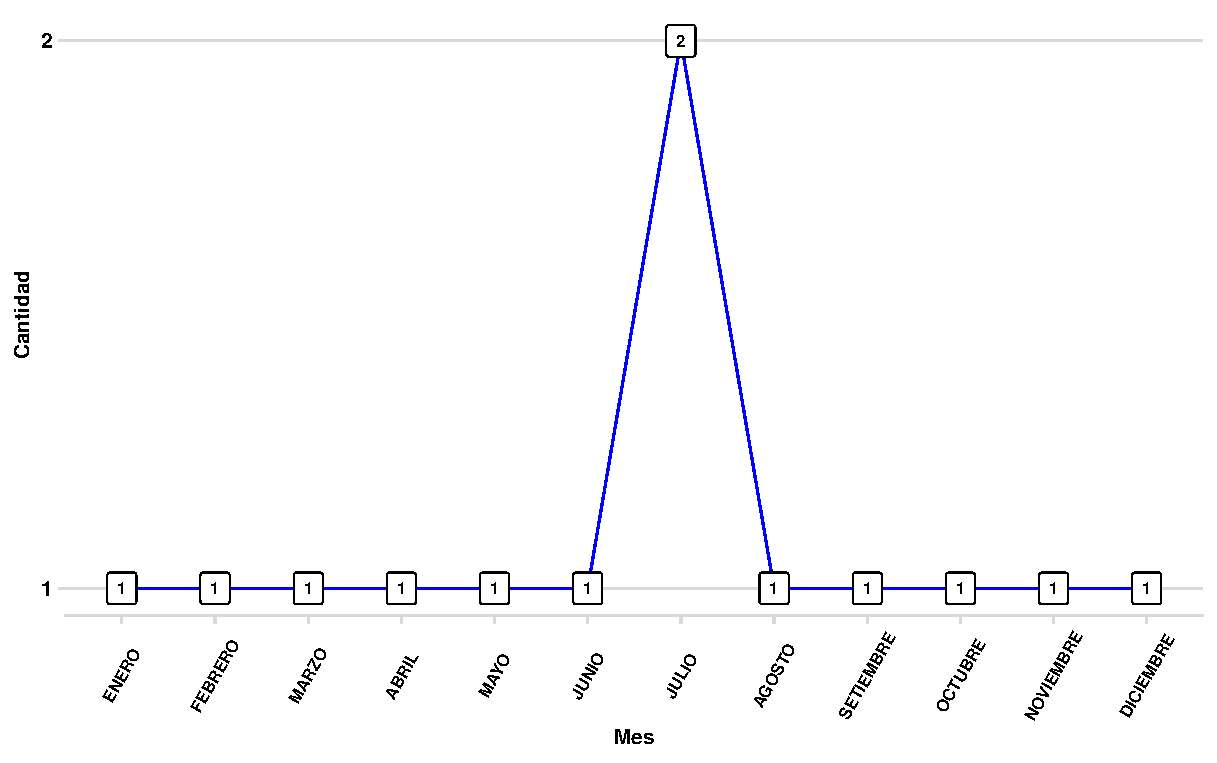
\includegraphics[width=15cm, height=5.95cm]{images/PROD010_demanda.pdf}}
  \label{fig:PROD010_demanda}
\end{figure}

La Figura \ref{fig:PROD010_demanda} muestra el diagrama de lineas que representa la evolución de la demanda del toner TNP80Y yellow por mes en el año 2024, se observa que la demanda tiene un comportamiento determinístico y sin estacionariedad ya que parece constante en los meses sin tendencia, tomando estos casos y el comportamiento de la demanda es necesario utilizar un \textsl{modelo determinístico EOQ}.

Tomando en cuenta la demanda total anual de la Tabla \ref{table:GrupoA_Area}, el costo de compra de la Tabla \ref{table:GrupoA_Costo_Compra}, el costo de preparación estimado de la Tabla \ref{table:GrupoA_Costo_Preparacion}, el costo de retención estimado de la Tabla \ref{table:GrupoA_Costo_Retencion} y tiempo de reabastecimiento del pedido brindado por el área de logística se tienen los siguientes valores:

\begin{itemize}
    \item \textbf{Demanda ($D$):} 13 unidades
    \item \textbf{Costo de compra ($C$):} S/ 720.00 por unidad
    \item \textbf{Costo de preparación ($K$):} S/ 11.51
    \item \textbf{Costo de retención ($h$):} S/ 7.76
    \item \textbf{Tiempo de entrega ($L$):} 1 día
\end{itemize}

Hallamos la cantidad de pedido óptima $y^*$ mediante la expresión (\ref{yopt}) de la siguiente manera
\begin{eqnarray}
    y^* &=& \sqrt{\frac{2KD}{h}} \nonumber
\end{eqnarray}
\begin{eqnarray}
    y^* &=& \sqrt{\frac{2(11.51)(13)}{7.76}} \nonumber \\
    y^* &=& 6.21 \nonumber \\
    y^* &\thickapprox& 6 \text{ unidades} \nonumber
\end{eqnarray}
De la misma forma hallemos el intervalo de pedido óptimo $T^*$ utilizando la expresión (\ref{Topt}) 
\begin{eqnarray}
    T^* &=& \sqrt{\frac{2K}{Dh}} \nonumber \\
    T^* &=& \sqrt{\frac{2(11.51)}{(13)(7.76)}} \nonumber \\
    T^* &=& 0.4777 \nonumber
\end{eqnarray}
Asimismo tomemos la demanda por día laborable (52 semanas * 5 días/semana = 260 días laborables) de tal forma que vemos el momento de cuando pedir
\begin{eqnarray}
    T^* &=& 0.4777 (260 \text{ días laborables}) \nonumber \\   
    T^* &=& 124.2 \nonumber \\
    T^* &\thickapprox& 124 \text{ días laborables} \nonumber
\end{eqnarray}
Ahora hallemos el costo mínimo total de inventario óptimo $CTI(y^*)$ usando la expresión (\ref{CTIopt}).
\begin{eqnarray}
    CTI(y^*) &=& \sqrt{2hKD} + DC \nonumber \\
    CTI(y^*) &=& \sqrt{2(7.76)(11.51)(13)} + (13)(720) \nonumber \\
    CTI(y^*) &=& \text{S/ 9,408.19} \nonumber
\end{eqnarray}
Por último hallemos el punto de reorden en base a la cantidad de pedido óptima y el tiempo de reabastecimiento de 1 día.
\begin{eqnarray}
    R &=& L_e D \nonumber \\
    R &=& (1) \left(\frac{13}{260 \text{ días laborables}} \right) \nonumber
\end{eqnarray}
\begin{eqnarray}
    R &=& 0.05 \nonumber \\
    R &\thickapprox& 0 \text{ unidades} \nonumber
\end{eqnarray}

Esto quiere decir que cuando el inventario del producto llegue a 0 unidades se deben de realizar el pedido de 6 unidades, del cual el tiempo de pedido debería ser cada 124 días laborables teniendo un costo total de S/ 9,408.19
\subsubsection{Campo quirúrgico para ojos desechable 100 cm x 70 cm}
El producto campo quirúrgico para ojos desechable 100 cm x 70 cm de Insumos generales del área de oftalmología es utilizado para las cirugías oftalmológicas realizadas en general, primeramente observemos la tendencia de la demanda a lo largo del año 2024 en el siguiente gráfico.

\begin{figure}[H]
  \caption{Evolución demanda: Campo quirúrgico para ojos desechable 100 cm x 70 cm de Insumos generales - oftalmología}
  {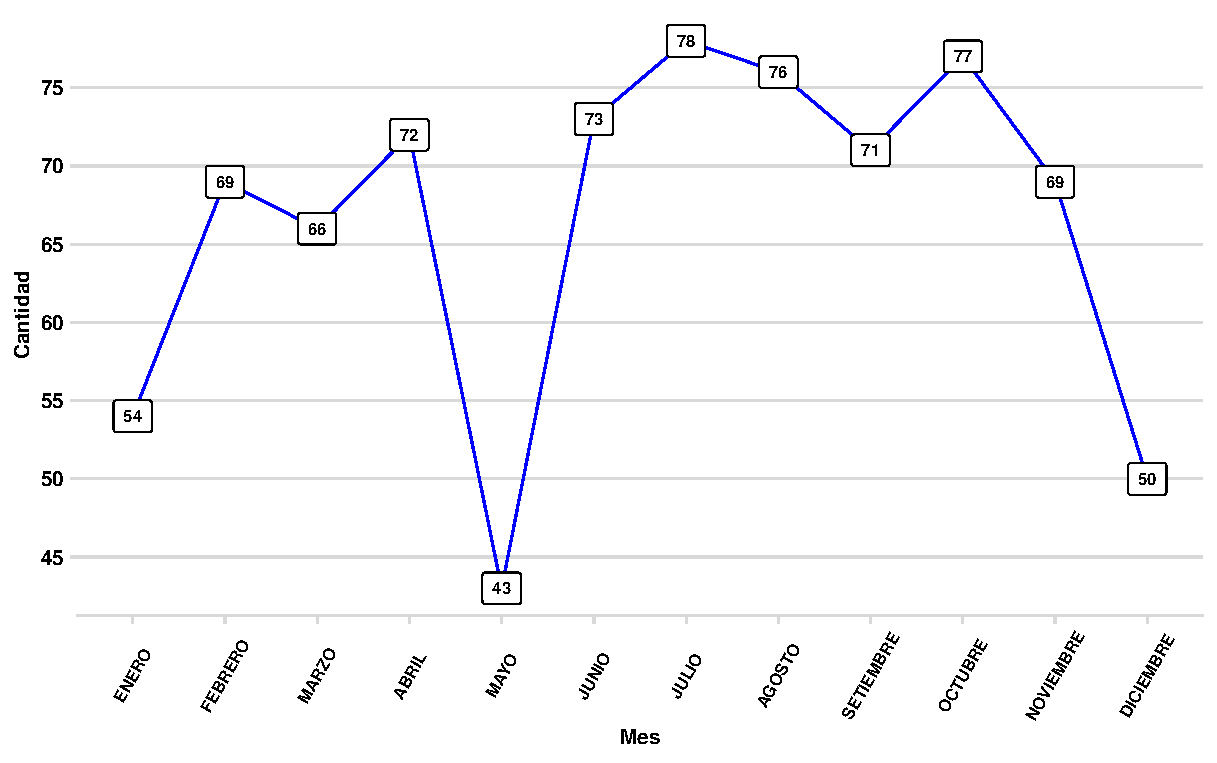
\includegraphics[width=15cm, height=5.95cm]{images/PROD011_demanda.pdf}}
  \label{fig:PROD011_demanda}
\end{figure}

La Figura \ref{fig:PROD011_demanda} muestra el diagrama de lineas que representa la evolución de la demanda del campo quirúrgico para ojos desechable 100 cm x 70 cm por mes en el año 2024, se observa que la demanda tiene un comportamiento determinístico a través de los meses del año, a excepción del mes de enero, mayo y diciembre en donde hubo puntos extremos bajos, asimismo no se observa una tendencia y solo estacionariedad en el tiempo, por lo que tomando estos casos y el comportamiento de la demanda es necesario utilizar un \textsl{modelo determinístico EOQ}.

Tomando en cuenta la demanda total anual de la Tabla \ref{table:GrupoA_Area}, el costo de compra de la Tabla \ref{table:GrupoA_Costo_Compra}, el costo de preparación estimado de la Tabla \ref{table:GrupoA_Costo_Preparacion}, el costo de retención estimado de la Tabla \ref{table:GrupoA_Costo_Retencion} y tiempo de reabastecimiento del pedido brindado por el área de logística se tienen los siguientes valores:

\begin{itemize}
    \item \textbf{Demanda ($D$):} 798 unidades
    \item \textbf{Costo de compra ($C$):} S/ 15.59 por unidad
    \item \textbf{Costo de preparación ($K$):} S/ 13.50
    \item \textbf{Costo de retención ($h$):} S/ 19.79
    \item \textbf{Tiempo de entrega ($L$):} 4 días
\end{itemize}

Hallamos la cantidad de pedido óptima $y^*$ mediante la expresión (\ref{yopt}) de la siguiente manera
\begin{eqnarray}
    y^* &=& \sqrt{\frac{2KD}{h}} \nonumber \\
    y^* &=& \sqrt{\frac{2(13.5)(798)}{19.79}} \nonumber \\
    y^* &=& 33.00 \nonumber \\
    y^* &\thickapprox& 33 \text{ unidades} \nonumber
\end{eqnarray}
De la misma forma hallemos el intervalo de pedido óptimo $T^*$ utilizando la expresión (\ref{Topt}) 
\begin{eqnarray}
    T^* &=& \sqrt{\frac{2K}{Dh}} \nonumber \\
    T^* &=& \sqrt{\frac{2(13.5)}{(798)(19.79)}} \nonumber \\
    T^* &=& 0.0413 \nonumber
\end{eqnarray}
Asimismo tomemos la demanda por día laborable (52 semanas * 5 días/semana = 260 días laborables) de tal forma que vemos el momento de cuando pedir
\begin{eqnarray}
    T^* &=& 0.0413 (260 \text{ días laborables}) \nonumber
\end{eqnarray}
\begin{eqnarray}
    T^* &=& 10.75 \nonumber \\
    T^* &\thickapprox& 11 \text{ días laborables} \nonumber
\end{eqnarray}
Ahora hallemos el costo mínimo total de inventario óptimo $CTI(y^*)$ usando la expresión (\ref{CTIopt}).
\begin{eqnarray}
    CTI(y^*) &=& \sqrt{2hKD} + DC \nonumber \\
    CTI(y^*) &=& \sqrt{2(19.79)(13.5)(798)} + (798)(15.59) \nonumber \\
    CTI(y^*) &=& \text{S/ 13,093.81} \nonumber
\end{eqnarray}
Por último hallemos el punto de reorden en base a la cantidad de pedido óptima y el tiempo de reabastecimiento de 4 días.
\begin{eqnarray}
    R &=& L_e D \nonumber \\
    R &=& (4) \left(\frac{798}{260 \text{ días laborables}} \right) \nonumber \\
    R &=& 12.28 \nonumber \\
    R &\thickapprox& 12 \text{ unidades} \nonumber
\end{eqnarray}

Esto quiere decir que cuando el inventario del producto llegue a 12 unidades se deben de realizar el pedido de 33 unidades, del cual el tiempo de pedido debería ser cada 11 días laborables teniendo un costo total de S/ 13,093.81
\subsubsection{Toner TNP80C cyan para Konica Minolta BIZHUB C-3320i}

El producto toner TNP80C cyan para Konica Minolta de Tintas del área de oftalmología es utilizado para las impresiones realizadas en el área de exámenes especiales en tomografías realizadas, primeramente observemos la tendencia de la demanda a lo largo del año 2024 en el siguiente gráfico.
\clearpage
\begin{figure}[H]
  \caption{Evolución demanda: Toner TNP80C cyan para Konica Minolta de Tintas - oftalmología}
  {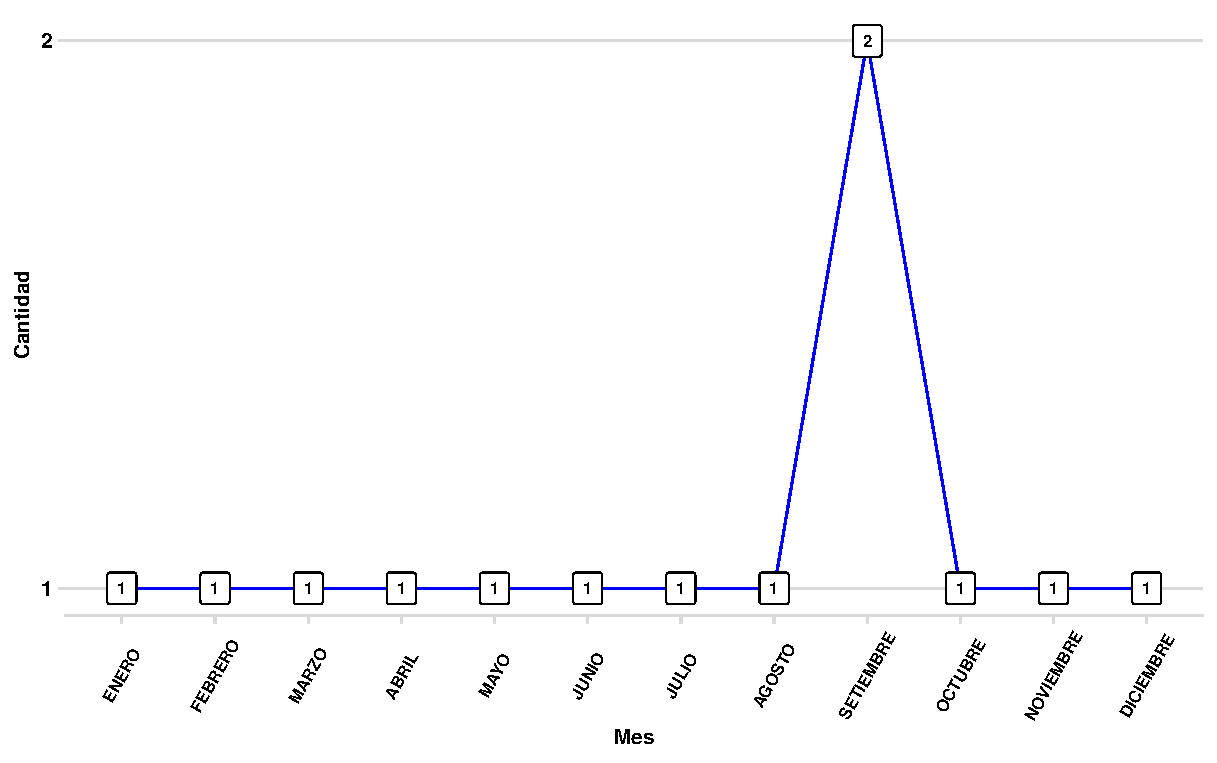
\includegraphics[width=15cm, height=5.95cm]{images/PROD012_demanda.pdf}}
  \label{fig:PROD012_demanda}
\end{figure}

La Figura \ref{fig:PROD012_demanda} muestra el diagrama de lineas que representa la evolución de la demanda del toner TNP80C cyan por mes en el año 2024, se observa que la demanda tiene un comportamiento determinístico y sin estacionariedad ya que parece constante en los meses sin tendencia, tomando estos casos y el comportamiento de la demanda es necesario utilizar un \textsl{modelo determinístico EOQ}.

Tomando en cuenta la demanda total anual de la Tabla \ref{table:GrupoA_Area}, el costo de compra de la Tabla \ref{table:GrupoA_Costo_Compra}, el costo de preparación estimado de la Tabla \ref{table:GrupoA_Costo_Preparacion}, el costo de retención estimado de la Tabla \ref{table:GrupoA_Costo_Retencion} y tiempo de reabastecimiento del pedido brindado por el área de logística se tienen los siguientes valores:

\begin{itemize}
    \item \textbf{Demanda ($D$):} 13 unidades
    \item \textbf{Costo de compra ($C$):} S/ 715.00 por unidad
    \item \textbf{Costo de preparación ($K$):} S/ 15.41
    \item \textbf{Costo de retención ($h$):} S/ 7.76
    \item \textbf{Tiempo de entrega ($L$):} 1 día
\end{itemize}

Hallamos la cantidad de pedido óptima $y^*$ mediante la expresión (\ref{yopt}) de la siguiente manera
\begin{eqnarray}
    y^* &=& \sqrt{\frac{2KD}{h}} \nonumber
\end{eqnarray}
\begin{eqnarray}
    y^* &=& \sqrt{\frac{2(15.41)(13)}{7.76}} \nonumber \\
    y^* &=& 7.19 \nonumber \\
    y^* &\thickapprox& 7 \text{ unidades} \nonumber
\end{eqnarray}
De la misma forma hallemos el intervalo de pedido óptimo $T^*$ utilizando la expresión (\ref{Topt}) 
\begin{eqnarray}
    T^* &=& \sqrt{\frac{2K}{Dh}} \nonumber \\
    T^* &=& \sqrt{\frac{2(15.41)}{(13)(7.76)}} \nonumber \\
    T^* &=& 0.5527 \nonumber
\end{eqnarray}
Asimismo tomemos la demanda por día laborable (52 semanas * 5 días/semana = 260 días laborables) de tal forma que vemos el momento de cuando pedir
\begin{eqnarray}
    T^* &=& 0.5527 (260 \text{ días laborables}) \nonumber \\   
    T^* &=& 143.71 \nonumber \\
    T^* &\thickapprox& 144 \text{ días laborables} \nonumber
\end{eqnarray}
Ahora hallemos el costo mínimo total de inventario óptimo $CTI(y^*)$ usando la expresión (\ref{CTIopt}).
\begin{eqnarray}
    CTI(y^*) &=& \sqrt{2hKD} + DC \nonumber \\
    CTI(y^*) &=& \sqrt{2(7.76)(15.41)(13)} + (13)(715) \nonumber \\
    CTI(y^*) &=& \text{S/ 9,350.76} \nonumber
\end{eqnarray}
Por último hallemos el punto de reorden en base a la cantidad de pedido óptima y el tiempo de reabastecimiento de 1 día.
\begin{eqnarray}
    R &=& L_e D \nonumber \\
    R &=& (1) \left(\frac{13}{260 \text{ días laborables}} \right) \nonumber
\end{eqnarray}
\begin{eqnarray}
    R &=& 0.05 \nonumber \\
    R &\thickapprox& 0 \text{ unidades} \nonumber
\end{eqnarray}

Esto quiere decir que cuando el inventario del producto llegue a 0 unidades se deben de realizar el pedido de 7 unidades, del cual el tiempo de pedido debería ser cada 144 días laborables teniendo un costo total de S/ 9,350.76
\subsubsection{Lentes de contacto - AIR optix día y noche}

El producto lentes de contacto - AIR optix día y noche de Insumos generales del área de oftalmología es utilizado generalmente en las cirugías de Pterigion usado para remover la carnosidad en la conjuntiva que llega a la córnea, también utilizado en algunas cirugías de catarata si es necesario, primeramente observemos la tendencia de la demanda a lo largo del año 2024 en el siguiente gráfico.

\begin{figure}[H]
  \caption{Evolución demanda: Lentes de contacto - AIR optix día y noche de Insumos generales - oftalmología}
  {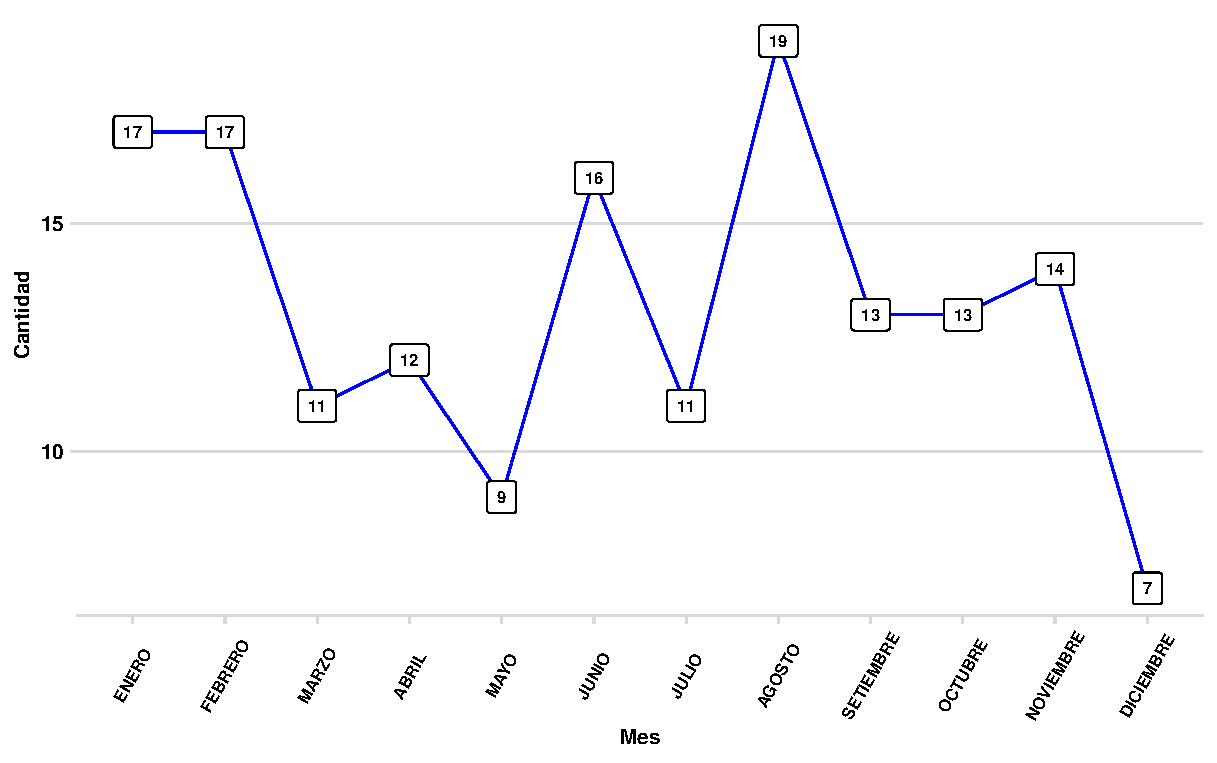
\includegraphics[width=15cm, height=5.95cm]{images/PROD013_demanda.pdf}}
  \label{fig:PROD013_demanda}
\end{figure}

La Figura \ref{fig:PROD013_demanda} muestra el diagrama de lineas que representa la evolución de la demanda del campo quirúrgico para ojos desechable 100 cm x 70 cm por mes en el año 2024, se observa que la demanda tiene un comportamiento determinístico a través de los meses del año, a excepción del mes de diciembre en donde se encuentra el valor más bajo, asimismo no se observa una tendencia y solo estacionariedad en el tiempo, por lo que tomando estos casos y el comportamiento de la demanda es necesario utilizar un \textsl{modelo determinístico EOQ}.

Tomando en cuenta la demanda total anual de la Tabla \ref{table:GrupoA_Area}, el costo de compra de la Tabla \ref{table:GrupoA_Costo_Compra}, el costo de preparación estimado de la Tabla \ref{table:GrupoA_Costo_Preparacion}, el costo de retención estimado de la Tabla \ref{table:GrupoA_Costo_Retencion} y tiempo de reabastecimiento del pedido brindado por el área de logística se tienen los siguientes valores:

\begin{itemize}
    \item \textbf{Demanda ($D$):} 159 unidades
    \item \textbf{Costo de compra ($C$):} S/ 143.37 por unidad
    \item \textbf{Costo de preparación ($K$):} S/ 1.90
    \item \textbf{Costo de retención ($h$):} S/ 6.42
    \item \textbf{Tiempo de entrega ($L$):} 3 días
\end{itemize}

Hallamos la cantidad de pedido óptima $y^*$ mediante la expresión (\ref{yopt}) de la siguiente manera
\begin{eqnarray}
    y^* &=& \sqrt{\frac{2KD}{h}} \nonumber \\
    y^* &=& \sqrt{\frac{2(1.9)(159)}{6.42}} \nonumber \\
    y^* &=& 9.7 \nonumber \\
    y^* &\thickapprox& 10 \text{ unidades} \nonumber
\end{eqnarray}
De la misma forma hallemos el intervalo de pedido óptimo $T^*$ utilizando la expresión (\ref{Topt}) 
\begin{eqnarray}
    T^* &=& \sqrt{\frac{2K}{Dh}} \nonumber \\
    T^* &=& \sqrt{\frac{2(1.9)}{(159)(6.42)}} \nonumber \\
    T^* &=& 0.0610 \nonumber
\end{eqnarray}
Asimismo tomemos la demanda por día laborable (52 semanas * 5 días/semana = 260 días laborables) de tal forma que vemos el momento de cuando pedir
\begin{eqnarray}
    T^* &=& 0.0610 (260 \text{ días laborables}) \nonumber
\end{eqnarray}
\begin{eqnarray}
    T^* &=& 15.86 \nonumber \\
    T^* &\thickapprox& 16 \text{ días laborables} \nonumber
\end{eqnarray}
Ahora hallemos el costo mínimo total de inventario óptimo $CTI(y^*)$ usando la expresión (\ref{CTIopt}).
\begin{eqnarray}
    CTI(y^*) &=& \sqrt{2hKD} + DC \nonumber \\
    CTI(y^*) &=& \sqrt{2(6.42)(1.9)(159)} + (159)(143.37) \nonumber \\
    CTI(y^*) &=& \text{S/ 22,858.11} \nonumber
\end{eqnarray}
Por último hallemos el punto de reorden en base a la cantidad de pedido óptima y el tiempo de reabastecimiento de 3 días.
\begin{eqnarray}
    R &=& L_e D \nonumber \\
    R &=& (3) \left(\frac{159}{260 \text{ días laborables}} \right) \nonumber \\
    R &=& 1.83 \nonumber \\
    R &\thickapprox& 2 \text{ unidades} \nonumber
\end{eqnarray}

Esto quiere decir que cuando el inventario del producto llegue a 2 unidades se deben de realizar el pedido de 10 unidades, del cual el tiempo de pedido debería ser cada 16 días laborables teniendo un costo total de S/ 22,858.11
\subsubsection{Toner Konica Minolta BIZHUB C-3320i Magenta}

El producto toner Konica Minolta BIZHUB C-3320i magenta de Tintas del área de oftalmología es utilizado para las impresiones realizadas en el área de exámenes especiales en tomografías realizadas, primeramente observemos la tendencia de la demanda a lo largo del año 2024 en el siguiente gráfico.
\clearpage
\begin{figure}[H]
  \caption{Evolución demanda: Toner Konica Minolta BIZHUB C-3320i de Tintas - oftalmología}
  {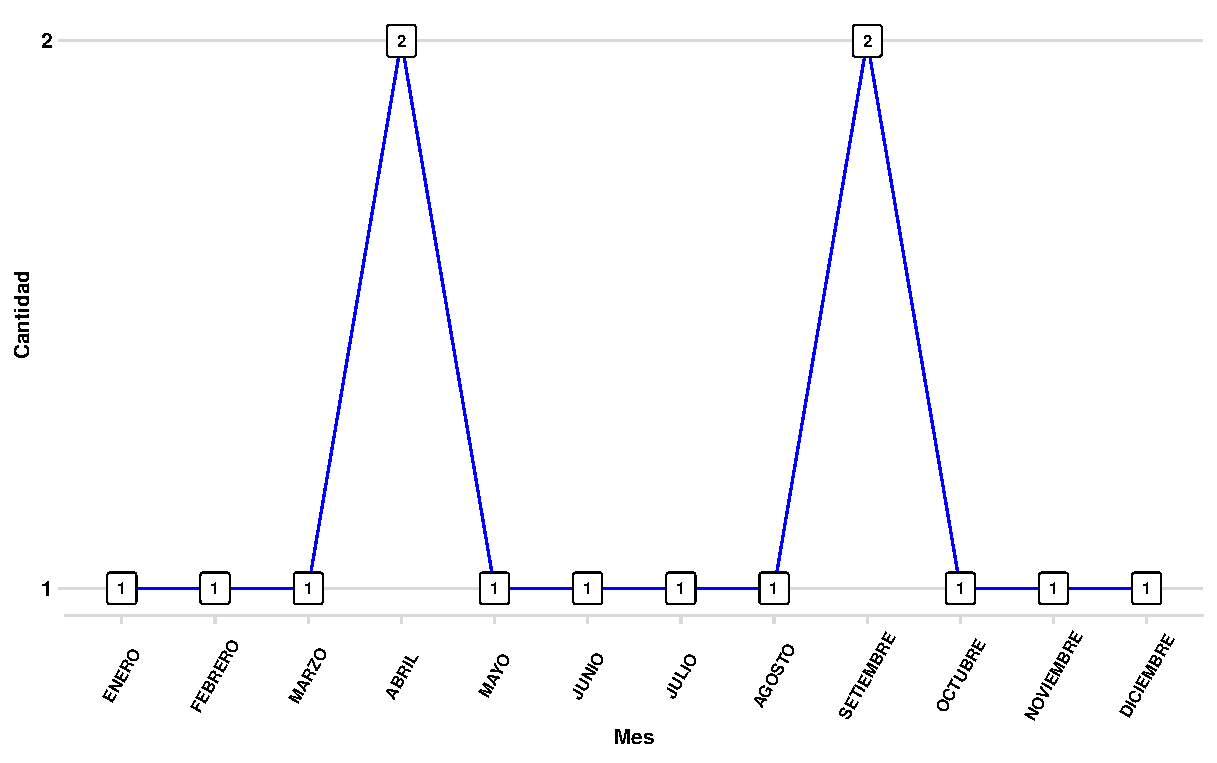
\includegraphics[width=15cm, height=5.95cm]{images/PROD014_demanda.pdf}}
  \label{fig:PROD014_demanda}
\end{figure}

La Figura \ref{fig:PROD014_demanda} muestra el diagrama de lineas que representa la evolución de la demanda del toner TNP80C cyan por mes en el año 2024, se observa que la demanda tiene un comportamiento determinístico y sin estacionariedad ya que parece constante en los meses sin tendencia, tomando estos casos y el comportamiento de la demanda es necesario utilizar un \textsl{modelo determinístico EOQ}.

Tomando en cuenta la demanda total anual de la Tabla \ref{table:GrupoA_Area}, el costo de compra de la Tabla \ref{table:GrupoA_Costo_Compra}, el costo de preparación estimado de la Tabla \ref{table:GrupoA_Costo_Preparacion}, el costo de retención estimado de la Tabla \ref{table:GrupoA_Costo_Retencion} y tiempo de reabastecimiento del pedido brindado por el área de logística se tienen los siguientes valores:

\begin{itemize}
    \item \textbf{Demanda ($D$):} 14 unidades
    \item \textbf{Costo de compra ($C$):} S/ 715.00 por unidad
    \item \textbf{Costo de preparación ($K$):} S/ 9.61
    \item \textbf{Costo de retención ($h$):} S/ 7.76
    \item \textbf{Tiempo de entrega ($L$):} 1 día
\end{itemize}

Hallamos la cantidad de pedido óptima $y^*$ mediante la expresión (\ref{yopt}) de la siguiente manera
\begin{eqnarray}
    y^* &=& \sqrt{\frac{2KD}{h}} \nonumber
\end{eqnarray}
\begin{eqnarray}
    y^* &=& \sqrt{\frac{2(9.61)(14)}{7.76}} \nonumber \\
    y^* &=& 5.89 \nonumber \\
    y^* &\thickapprox& 6 \text{ unidades} \nonumber
\end{eqnarray}
De la misma forma hallemos el intervalo de pedido óptimo $T^*$ utilizando la expresión (\ref{Topt}) 
\begin{eqnarray}
    T^* &=& \sqrt{\frac{2K}{Dh}} \nonumber \\
    T^* &=& \sqrt{\frac{2(9.61)}{(14)(7.76)}} \nonumber \\
    T^* &=& 0.4206 \nonumber
\end{eqnarray}
Asimismo tomemos la demanda por día laborable (52 semanas * 5 días/semana = 260 días laborables) de tal forma que vemos el momento de cuando pedir
\begin{eqnarray}
    T^* &=& 0.4206 (260 \text{ días laborables}) \nonumber \\   
    T^* &=& 109.36 \nonumber \\
    T^* &\thickapprox& 109 \text{ días laborables} \nonumber
\end{eqnarray}
Ahora hallemos el costo mínimo total de inventario óptimo $CTI(y^*)$ usando la expresión (\ref{CTIopt}).
\begin{eqnarray}
    CTI(y^*) &=& \sqrt{2hKD} + DC \nonumber \\
    CTI(y^*) &=& \sqrt{2(7.76)(9.61)(14)} + (14)(715) \nonumber \\
    CTI(y^*) &=& \text{S/ 10,055.70} \nonumber
\end{eqnarray}
Por último hallemos el punto de reorden en base a la cantidad de pedido óptima y el tiempo de reabastecimiento de 1 día.
\begin{eqnarray}
    R &=& L_e D \nonumber \\
    R &=& (1) \left(\frac{14}{260 \text{ días laborables}} \right) \nonumber
\end{eqnarray}
\begin{eqnarray}
    R &=& 0.05 \nonumber \\
    R &\thickapprox& 0 \text{ unidades} \nonumber
\end{eqnarray}

Esto quiere decir que cuando el inventario del producto llegue a 0 unidades se deben de realizar el pedido de 6 unidades, del cual el tiempo de pedido debería ser cada 109 días laborables teniendo un costo total de S/ 10,055.70
\subsubsection{Solución salina equilibrada (BSS) en botella de vidrio 500 ml}

El producto solución salina equilibrada (BSS) en botella de vidrio de 500 ml de Catarata del área de oftalmología es utilizado generalmente en las cirugías del área de oftalmología realizadas, primeramente observemos la tendencia de la demanda a lo largo del año 2024 en el siguiente gráfico.

\begin{figure}[H]
  \caption{Evolución demanda: Solución salina equilibrada (BSS) en botella de vidrio 500 ml de Catarata - oftalmología}
  {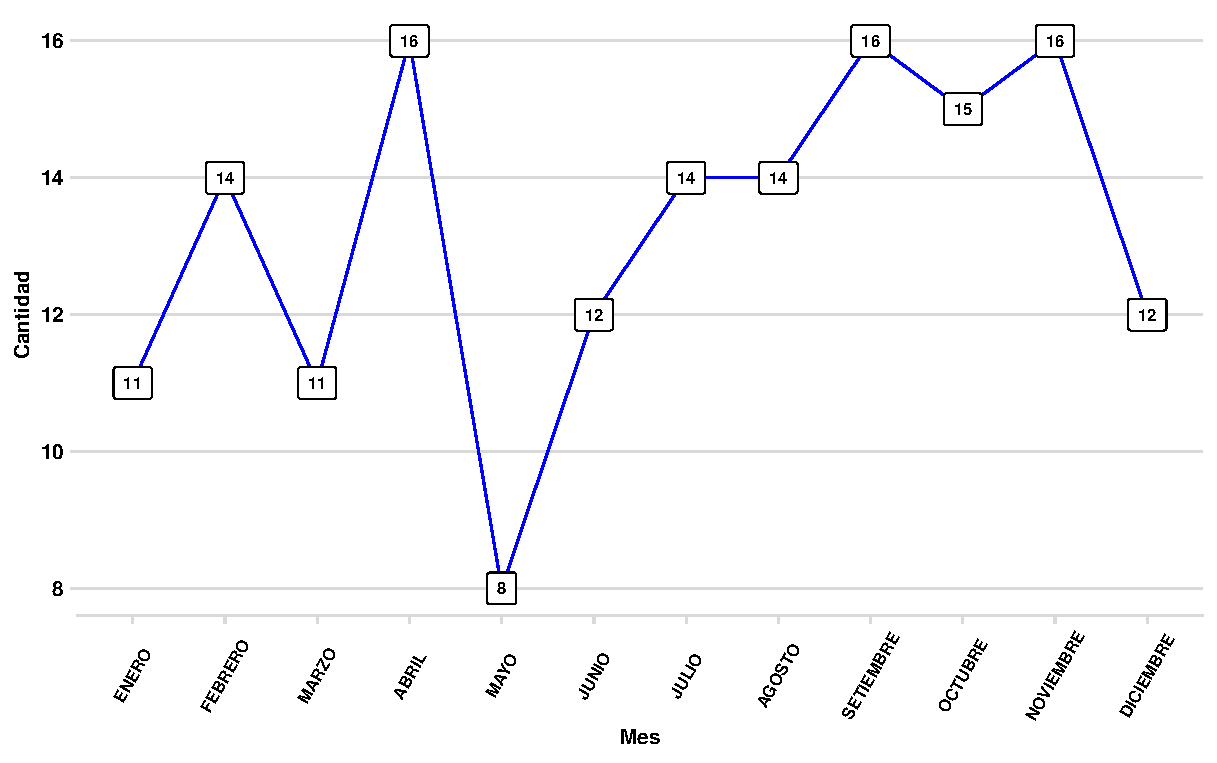
\includegraphics[width=15cm, height=5.95cm]{images/PROD015_demanda.pdf}}
  \label{fig:PROD015_demanda}
\end{figure}

La Figura \ref{fig:PROD015_demanda} muestra el diagrama de lineas que representa la evolución de la demanda sobre la solución salina equilibrada (BSS) por mes en el año 2024, se observa que la demanda tiene un comportamiento determinístico a través de los meses del año, a excepción del mes de mayo en donde se encuentra el valor más bajo, asimismo no se observa una tendencia y solo estacionariedad en el tiempo, por lo que tomando estos casos y el comportamiento de la demanda es necesario utilizar un \textsl{modelo determinístico EOQ}.

Tomando en cuenta la demanda total anual de la Tabla \ref{table:GrupoA_Area}, el costo de compra de la Tabla \ref{table:GrupoA_Costo_Compra}, el costo de preparación estimado de la Tabla \ref{table:GrupoA_Costo_Preparacion}, el costo de retención estimado de la Tabla \ref{table:GrupoA_Costo_Retencion} y tiempo de reabastecimiento del pedido brindado por el área de logística se tienen los siguientes valores:

\begin{itemize}
    \item \textbf{Demanda ($D$):} 159 unidades
    \item \textbf{Costo de compra ($C$):} S/ 290.00 por unidad
    \item \textbf{Costo de preparación ($K$):} S/ 5.80
    \item \textbf{Costo de retención ($h$):} S/ 18.19
    \item \textbf{Tiempo de entrega ($L$):} 7 días
\end{itemize}

Hallamos la cantidad de pedido óptima $y^*$ mediante la expresión (\ref{yopt}) de la siguiente manera
\begin{eqnarray}
    y^* &=& \sqrt{\frac{2KD}{h}} \nonumber \\
    y^* &=& \sqrt{\frac{2(5.8)(159)}{18.19}} \nonumber \\
    y^* &=& 10.07 \nonumber \\
    y^* &\thickapprox& 10 \text{ unidades} \nonumber
\end{eqnarray}
De la misma forma hallemos el intervalo de pedido óptimo $T^*$ utilizando la expresión (\ref{Topt}) 
\begin{eqnarray}
    T^* &=& \sqrt{\frac{2K}{Dh}} \nonumber \\
    T^* &=& \sqrt{\frac{2(5.8)}{(159)(18.19)}} \nonumber \\
    T^* &=& 0.0633 \nonumber
\end{eqnarray}
Asimismo tomemos la demanda por día laborable (52 semanas * 5 días/semana = 260 días laborables) de tal forma que vemos el momento de cuando pedir
\begin{eqnarray}
    T^* &=& 0.0633 (260 \text{ días laborables}) \nonumber
\end{eqnarray}
\begin{eqnarray}
    T^* &=& 16.47 \nonumber \\
    T^* &\thickapprox& 16 \text{ días laborables} \nonumber
\end{eqnarray}
Ahora hallemos el costo mínimo total de inventario óptimo $CTI(y^*)$ usando la expresión (\ref{CTIopt}).
\begin{eqnarray}
    CTI(y^*) &=& \sqrt{2hKD} + DC \nonumber \\
    CTI(y^*) &=& \sqrt{2(18.19)(5.8)(159)} + (159)(290) \nonumber \\
    CTI(y^*) &=& \text{S/ 46,293.17} \nonumber
\end{eqnarray}
Por último hallemos el punto de reorden en base a la cantidad de pedido óptima y el tiempo de reabastecimiento de 7 días.
\begin{eqnarray}
    R &=& L_e D \nonumber \\
    R &=& (7) \left(\frac{159}{260 \text{ días laborables}} \right) \nonumber \\
    R &=& 4.28 \nonumber \\
    R &\thickapprox& 4 \text{ unidades} \nonumber
\end{eqnarray}

Esto quiere decir que cuando el inventario del producto llegue a 4 unidades se deben de realizar el pedido de 10 unidades, del cual el tiempo de pedido debería ser cada 16 días laborables teniendo un costo total de S/ 46,293.17
\subsubsection{Campo quirúrgico 100 x 120 cm}

El producto campo quirúrgico 100 x 120 cm de Insumos generales del área de oftalmología es utilizado generalmente en las cirugías del área de oftalmología realizadas, primeramente observemos la tendencia de la demanda a lo largo del año 2024 en el siguiente gráfico.
\clearpage
\begin{figure}[H]
  \caption{Evolución demanda: Campo quirúrgico 100 x 120 cm de Insumos generales - oftalmología}
  {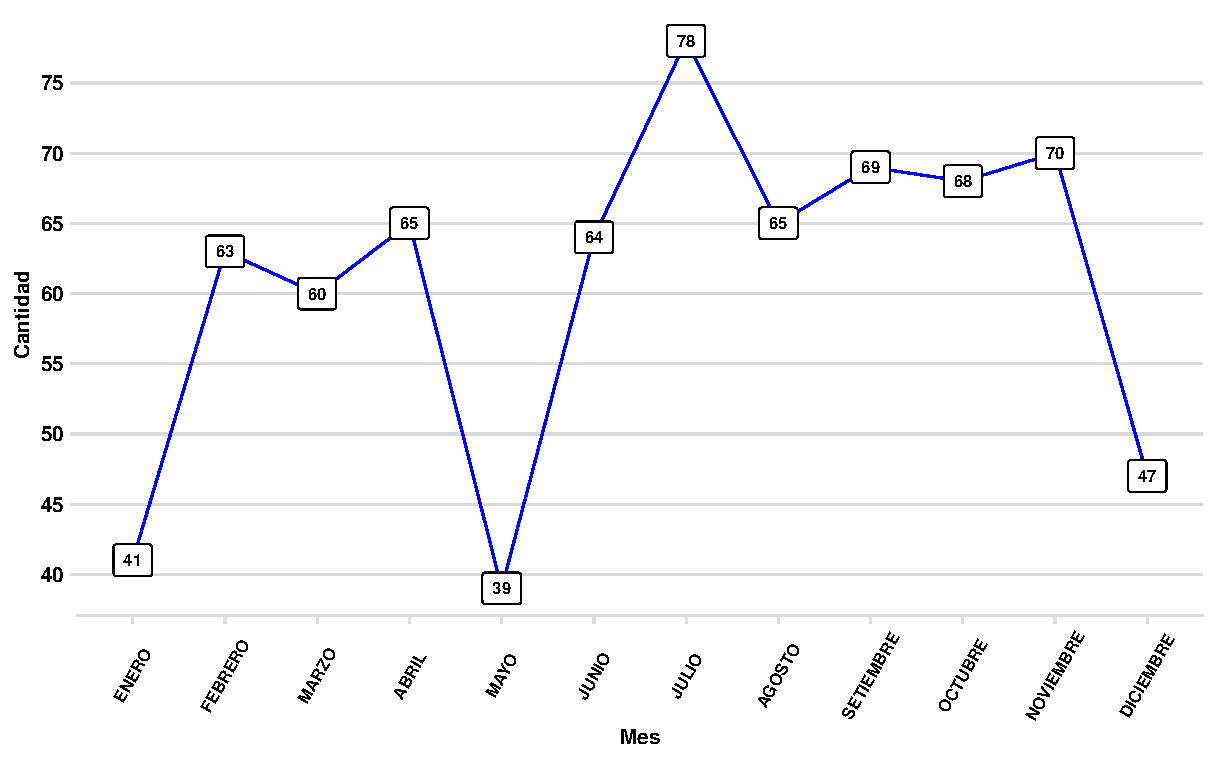
\includegraphics[width=15cm, height=5.95cm]{images/PROD016_demanda.pdf}}
  \label{fig:PROD016_demanda}
\end{figure}

La Figura \ref{fig:PROD016_demanda} muestra el diagrama de lineas que representa la evolución de la demanda del campo quirúrgico 100 x 120 cm por mes en el año 2024, se observa que la demanda tiene un comportamiento determinístico a través de los meses del año, a excepción de los meses de enero, mayo y diciembre en los cuales se presentan valores extremos bajos, asimismo no se observa una tendencia y solo estacionariedad en el tiempo, por lo que tomando estos casos y el comportamiento de la demanda es necesario utilizar un \textsl{modelo determinístico EOQ}.

Tomando en cuenta la demanda total anual de la Tabla \ref{table:GrupoA_Area}, el costo de compra de la Tabla \ref{table:GrupoA_Costo_Compra}, el costo de preparación estimado de la Tabla \ref{table:GrupoA_Costo_Preparacion}, el costo de retención estimado de la Tabla \ref{table:GrupoA_Costo_Retencion} y tiempo de reabastecimiento del pedido brindado por el área de logística se tienen los siguientes valores:

\begin{itemize}
    \item \textbf{Demanda ($D$):} 729 unidades
    \item \textbf{Costo de compra ($C$):} S/ 14.00 por unidad
    \item \textbf{Costo de preparación ($K$):} S/ 3.80
    \item \textbf{Costo de retención ($h$):} S/ 2.14
    \item \textbf{Tiempo de entrega ($L$):} 7 días
\end{itemize}

Hallamos la cantidad de pedido óptima $y^*$ mediante la expresión (\ref{yopt}) de la siguiente manera
\clearpage
\begin{eqnarray}
    y^* &=& \sqrt{\frac{2KD}{h}} \nonumber \\
    y^* &=& \sqrt{\frac{2(3.8)(729)}{2.14}} \nonumber \\
    y^* &=& 50.88 \nonumber \\
    y^* &\thickapprox& 51 \text{ unidades} \nonumber
\end{eqnarray}
De la misma forma hallemos el intervalo de pedido óptimo $T^*$ utilizando la expresión (\ref{Topt}) 
\begin{eqnarray}
    T^* &=& \sqrt{\frac{2K}{Dh}} \nonumber \\
    T^* &=& \sqrt{\frac{2(3.8)}{(729)(2.14)}} \nonumber \\
    T^* &=& 0.0698 \nonumber
\end{eqnarray}
Asimismo tomemos la demanda por día laborable (52 semanas * 5 días/semana = 260 días laborables) de tal forma que vemos el momento de cuando pedir
\begin{eqnarray}
    T^* &=& 0.0698 (260 \text{ días laborables}) \nonumber \\   
    T^* &=& 18.15 \nonumber \\
    T^* &\thickapprox& 18 \text{ días laborables} \nonumber
\end{eqnarray}
Ahora hallemos el costo mínimo total de inventario óptimo $CTI(y^*)$ usando la expresión (\ref{CTIopt}).
\begin{eqnarray}
    CTI(y^*) &=& \sqrt{2hKD} + DC \nonumber \\
    CTI(y^*) &=& \sqrt{2(2.14)(3.8)(729)} + (729)(14) \nonumber \\
    CTI(y^*) &=& \text{S/ 10,314.89} \nonumber
\end{eqnarray}
Por último hallemos el punto de reorden en base a la cantidad de pedido óptima y el tiempo de reabastecimiento de 7 días.
\clearpage
\begin{eqnarray}
    R &=& L_e D \nonumber \\
    R &=& (7) \left(\frac{729}{260 \text{ días laborables}} \right) \nonumber \\
    R &=& 19.63 \nonumber \\
    R &\thickapprox& 20 \text{ unidades} \nonumber
\end{eqnarray}

Esto quiere decir que cuando el inventario del producto llegue a 20 unidades se deben de realizar el pedido de 51 unidades, del cual el tiempo de pedido debería ser cada 18 días laborables teniendo un costo total de S/ 10,314.89
\subsubsection{Azul de tripan 0.06$\%$ - 0.6 mg VIAL x 1ml / OCUBLU - TRY}

El producto azul de tripan 0.06$\%$ - 0.6 mg VIAL x 1 ml de Catarata del área de oftalmología es utilizado para la cirugía de facoemulsificación y extracción manual de catarata con incisión pequeña que son las cirugías para la extracción de la catarata, primeramente observemos la tendencia de la demanda a lo largo del año 2024 en el siguiente gráfico.

\begin{figure}[H]
  \caption{Evolución demanda: Azul de tripan 0.06$\%$ - 0.6 mg VIAL x 1 ml / OCUBLU - TRY de Catarata - oftalmología}
  {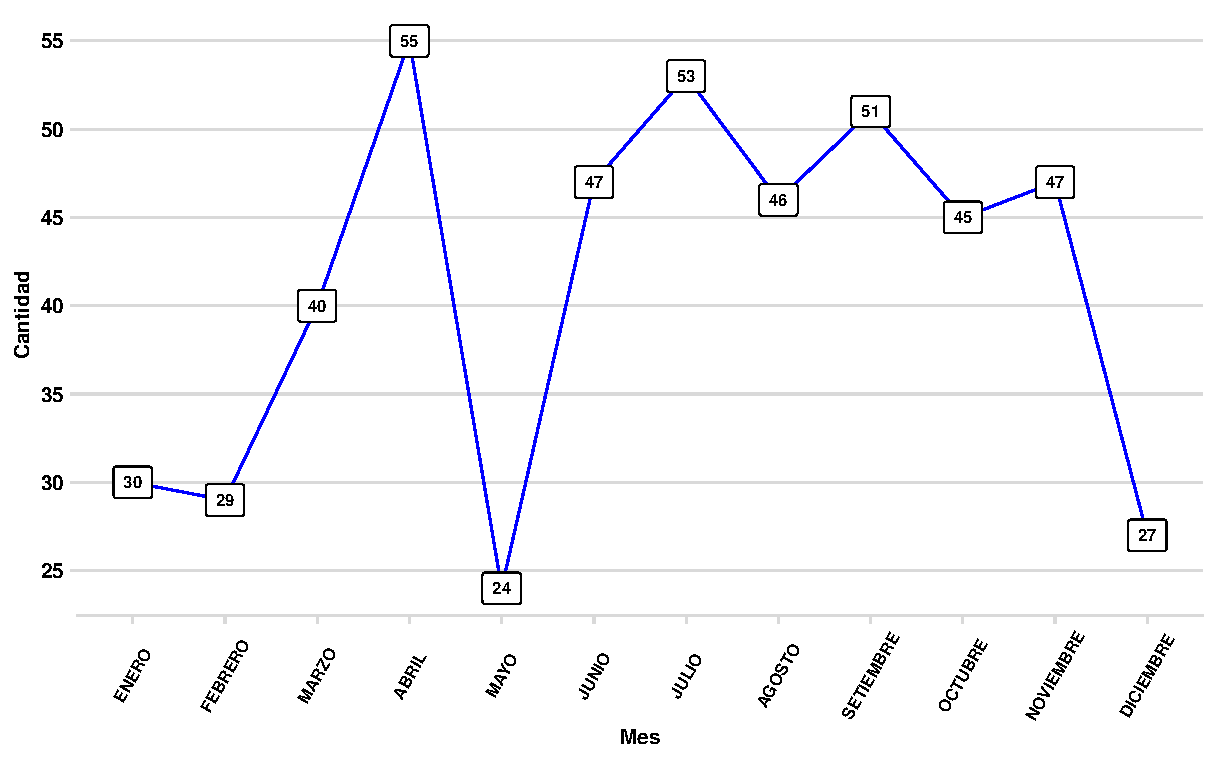
\includegraphics[width=15cm, height=5.95cm]{images/PROD017_demanda.pdf}}
  \label{fig:PROD017_demanda}
\end{figure}

La Figura \ref{fig:PROD017_demanda} muestra el diagrama de lineas que representa la evolución de la demanda del azul de tripan 0.06$\%$ por mes en el año 2024, se observa que la demanda tiene un comportamiento determinístico a través de los meses del año, a excepción de los meses de enero, febrero, mayo y diciembre en los cuales se tienen valores extremos bajos, asimismo no se observa una tendencia y solo estacionariedad en el tiempo, por lo que tomando estos casos y el comportamiento de la demanda es necesario utilizar un \textsl{modelo determinístico EOQ}.

Tomando en cuenta la demanda total anual de la Tabla \ref{table:GrupoA_Area}, el costo de compra de la Tabla \ref{table:GrupoA_Costo_Compra}, el costo de preparación estimado de la Tabla \ref{table:GrupoA_Costo_Preparacion}, el costo de retención estimado de la Tabla \ref{table:GrupoA_Costo_Retencion} y tiempo de reabastecimiento del pedido brindado por el área de logística se tienen los siguientes valores:

\begin{itemize}
    \item \textbf{Demanda ($D$):} 494 unidades
    \item \textbf{Costo de compra ($C$):} S/ 400.00 por unidad
    \item \textbf{Costo de preparación ($K$):} S/ 9.61
    \item \textbf{Costo de retención ($h$):} S/ 2.41
    \item \textbf{Tiempo de entrega ($L$):} 7 días
\end{itemize}

Hallamos la cantidad de pedido óptima $y^*$ mediante la expresión (\ref{yopt}) de la siguiente manera
\begin{eqnarray}
    y^* &=& \sqrt{\frac{2KD}{h}} \nonumber \\
    y^* &=& \sqrt{\frac{2(9.61)(494)}{2.41}} \nonumber \\
    y^* &=& 62.77 \nonumber \\
    y^* &\thickapprox& 63 \text{ unidades} \nonumber
\end{eqnarray}
De la misma forma hallemos el intervalo de pedido óptimo $T^*$ utilizando la expresión (\ref{Topt}) 
\begin{eqnarray}
    T^* &=& \sqrt{\frac{2K}{Dh}} \nonumber \\
    T^* &=& \sqrt{\frac{2(9.61)}{(494)(2.41)}} \nonumber \\
    T^* &=& 0.1271 \nonumber
\end{eqnarray}
\clearpage
\noindent Asimismo tomemos la demanda por día laborable (52 semanas * 5 días/semana = 260 días laborables) de tal forma que vemos el momento de cuando pedir
\begin{eqnarray}
    T^* &=& 0.1271 (260 \text{ días laborables}) \nonumber \\   
    T^* &=& 33.04 \nonumber \\
    T^* &\thickapprox& 33 \text{ días laborables} \nonumber
\end{eqnarray}
Ahora hallemos el costo mínimo total de inventario óptimo $CTI(y^*)$ usando la expresión (\ref{CTIopt}).
\begin{eqnarray}
    CTI(y^*) &=& \sqrt{2hKD} + DC \nonumber \\
    CTI(y^*) &=& \sqrt{2(2.41)(9.61)(494)} + (494)(400) \nonumber \\
    CTI(y^*) &=& \text{S/ 197,751.27} \nonumber
\end{eqnarray}
Por último hallemos el punto de reorden en base a la cantidad de pedido óptima y el tiempo de reabastecimiento de 7 días.
\begin{eqnarray}
    R &=& L_e D \nonumber \\
    R &=& (7) \left(\frac{494}{260 \text{ días laborables}} \right) \nonumber \\
    R &=& 13.30 \nonumber \\
    R &\thickapprox& 13 \text{ unidades} \nonumber
\end{eqnarray}

Esto quiere decir que cuando el inventario del producto llegue a 13 unidades se deben de realizar el pedido de 63 unidades, del cual el tiempo de pedido debería ser cada 33 días laborables teniendo un costo total de S/ 197,751.27

\subsubsection{Agua destilada y/o desionizada}

El producto agua destilada y/o desionizada de Esterilización del área de oftalmología es utilizado para el área de oftalmología en los procedimientos realizados, primeramente observemos la tendencia de la demanda a lo largo del año 2024 en el siguiente gráfico.
\clearpage
\begin{figure}[H]
  \caption{Evolución demanda: Agua destilada y/o desionizada de Esterilización - oftalmología}
  {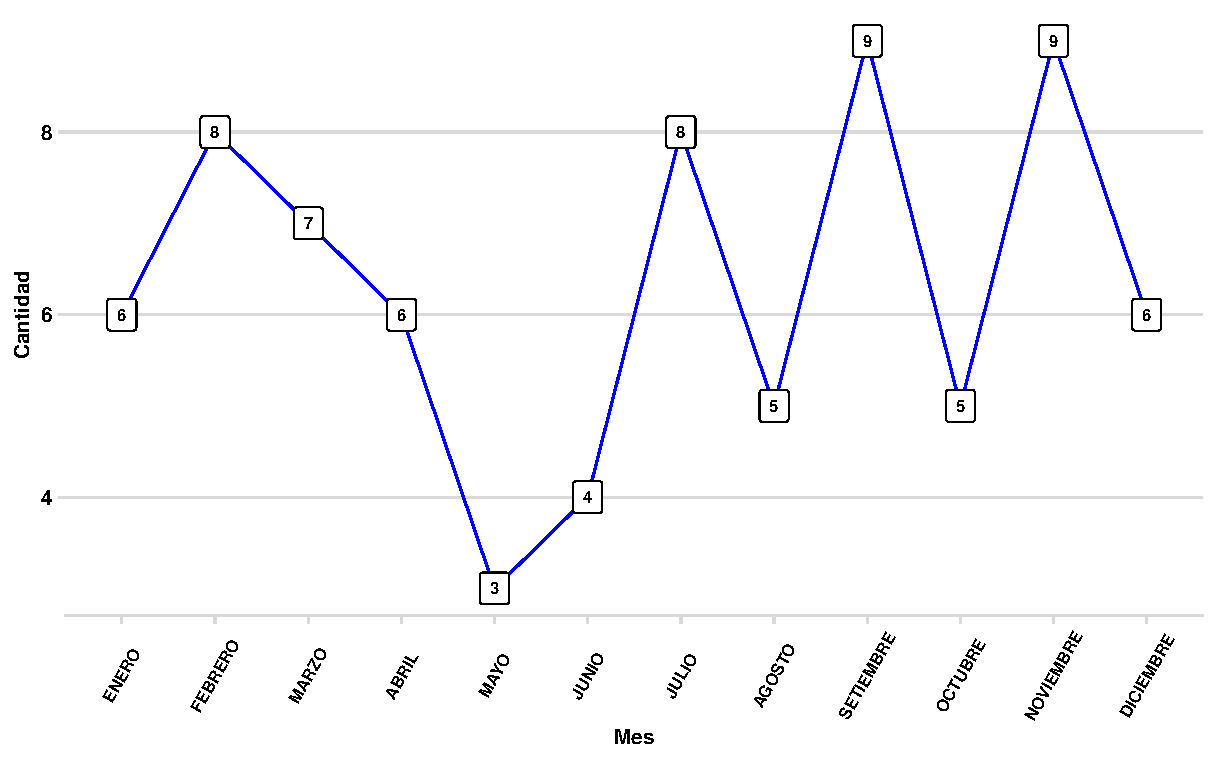
\includegraphics[width=15cm, height=5.95cm]{images/PROD018_demanda.pdf}}
  \label{fig:PROD018_demanda}
\end{figure}

La Figura \ref{fig:PROD018_demanda} muestra el diagrama de lineas que representa la evolución de la demanda del agua destilada por mes en el año 2024, se observa que la demanda tiene un comportamiento determinístico a través de los meses del año, a excepción del mes de mayo en donde se tuvo el punto más bajo, asimismo no se observa una tendencia y solo estacionariedad en el tiempo, por lo que tomando estos casos y el comportamiento de la demanda es necesario utilizar un \textsl{modelo determinístico EOQ}.

Tomando en cuenta la demanda total anual de la Tabla \ref{table:GrupoA_Area}, el costo de compra de la Tabla \ref{table:GrupoA_Costo_Compra}, el costo de preparación estimado de la Tabla \ref{table:GrupoA_Costo_Preparacion}, el costo de retención estimado de la Tabla \ref{table:GrupoA_Costo_Retencion} y tiempo de reabastecimiento del pedido brindado por el área de logística se tienen los siguientes valores:

\begin{itemize}
    \item \textbf{Demanda ($D$):} 76 unidades
    \item \textbf{Costo de compra ($C$):} S/ 39.84 por unidad
    \item \textbf{Costo de preparación ($K$):} S/ 11.51
    \item \textbf{Costo de retención ($h$):} S/ 473.40
    \item \textbf{Tiempo de entrega ($L$):} 7 días
\end{itemize}

Hallamos la cantidad de pedido óptima $y^*$ mediante la expresión (\ref{yopt}) de la siguiente manera
\clearpage
\begin{eqnarray}
    y^* &=& \sqrt{\frac{2KD}{h}} \nonumber \\
    y^* &=& \sqrt{\frac{2(11.51)(76)}{473.4}} \nonumber \\
    y^* &=& 1.92 \nonumber \\
    y^* &\thickapprox& 2 \text{ unidades} \nonumber
\end{eqnarray}
De la misma forma hallemos el intervalo de pedido óptimo $T^*$ utilizando la expresión (\ref{Topt}) 
\begin{eqnarray}
    T^* &=& \sqrt{\frac{2K}{Dh}} \nonumber \\
    T^* &=& \sqrt{\frac{2(11.51)}{(76)(473.4)}} \nonumber \\
    T^* &=& 0.0253 \nonumber
\end{eqnarray}
Asimismo tomemos la demanda por día laborable (52 semanas * 5 días/semana = 260 días laborables) de tal forma que vemos el momento de cuando pedir
\begin{eqnarray}
    T^* &=& 0.0253 (260 \text{ días laborables}) \nonumber \\   
    T^* &=& 6.58 \nonumber \\
    T^* &\thickapprox& 7 \text{ días laborables} \nonumber
\end{eqnarray}
Ahora hallemos el costo mínimo total de inventario óptimo $CTI(y^*)$ usando la expresión (\ref{CTIopt}).
\begin{eqnarray}
    CTI(y^*) &=& \sqrt{2hKD} + DC \nonumber \\
    CTI(y^*) &=& \sqrt{2(473.4)(11.51)(76)} + (76)(39.84) \nonumber \\
    CTI(y^*) &=& \text{S/ 3,937.91} \nonumber
\end{eqnarray}
Por último hallemos el punto de reorden en base a la cantidad de pedido óptima y el tiempo de reabastecimiento de 7 días.
\clearpage
\begin{eqnarray}
    R &=& L_e D \nonumber \\
    R &=& (7) \left(\frac{76}{260 \text{ días laborables}} \right) \nonumber \\
    R &=& 2.05 \nonumber \\
    R &\thickapprox& 2 \text{ unidades} \nonumber
\end{eqnarray}

Esto quiere decir que cuando el inventario del producto llegue a 2 unidades se deben de realizar el pedido de 2 unidades, del cual el tiempo de pedido debería ser cada 7 días laborables teniendo un costo total de S/ 3,937.91

\section{Generación del aplicativo web}
Como última parte se generará el aplicativo en Shiny que ayudará en el seguimiento no solo de los productos analizados anteriormente, sino también de nuevos productos que el centro de salud también requiera aplicar en su política de inventarios.

El aplicativo se desarrolló en el lenguaje R debido a su potencia en análisis estadístico y modelado matemático, permitiendo combinar de manera eficiente cálculos, visualizaciones y lógica de decisión en un solo entorno. De tal forma que se contribuye a la optimización de procesos de gestión de inventarios al facilitar una interfaz intuitiva para el usuario que automatize tareas que requieran intervención manual.

Para el desarrollo se empleó \textsl{RShiny}, un paquete de R que permite la creación de aplicaciones web interactivas, el cual tuvo las siguientes etapas:

\begin{enumerate}
    \item Diseño de la interfaz de usuario \textsl{(UI)} en el que se definieron los menús, paneles, filtros, ubicación de gráficos y tablas.
    \item Definición del servidor \textsl{(server)} en el que colocaron las funciones para procesar la lógica computacional, conectando los inputs del usuario con los outputs correspondientes.
    \item Carga y limpieza de datos en el que se tiene el procesamiento del archivo que se subirá para realizar el análisis, así como las debidas transformaciones y funciones que sean necesarias.
    \item Implementación de modelo de inventarios en el que se crearon funciones para realizar las políticas de inventarios tomando en cuenta el modelo EOQ clásico, EOQ con escasez y EOQ probabilizado.
    \item Visualización de resultados a través de gráficos, tablas e informaciones que permitan el monitoreo del inventario.
    \item Pruebas funcionales realizadas para asegurar la estabilidad de la aplicación y validación que pueda necesitar.
    \item Despliegue del aplicativo, ejecutandose en el servidor de Shiny con el plan básico gratuito, el enlace del aplicativo es el siguiente \url{https://kevin-heberth-haquehua-apaza.shinyapps.io/App_Inventario_Fuente_UNSAAC/}
\end{enumerate}

\subsection{Presentación del aplicativo}
Como primera parte se tiene la presentación del aplicativo web, mostrado cuando se accede al enlace, en esta parte se da una breve reseña de las funciones que contiene el aplicativo de inventario.
\begin{figure}[H]
  \caption{Información general del aplicativo de inventario}
  {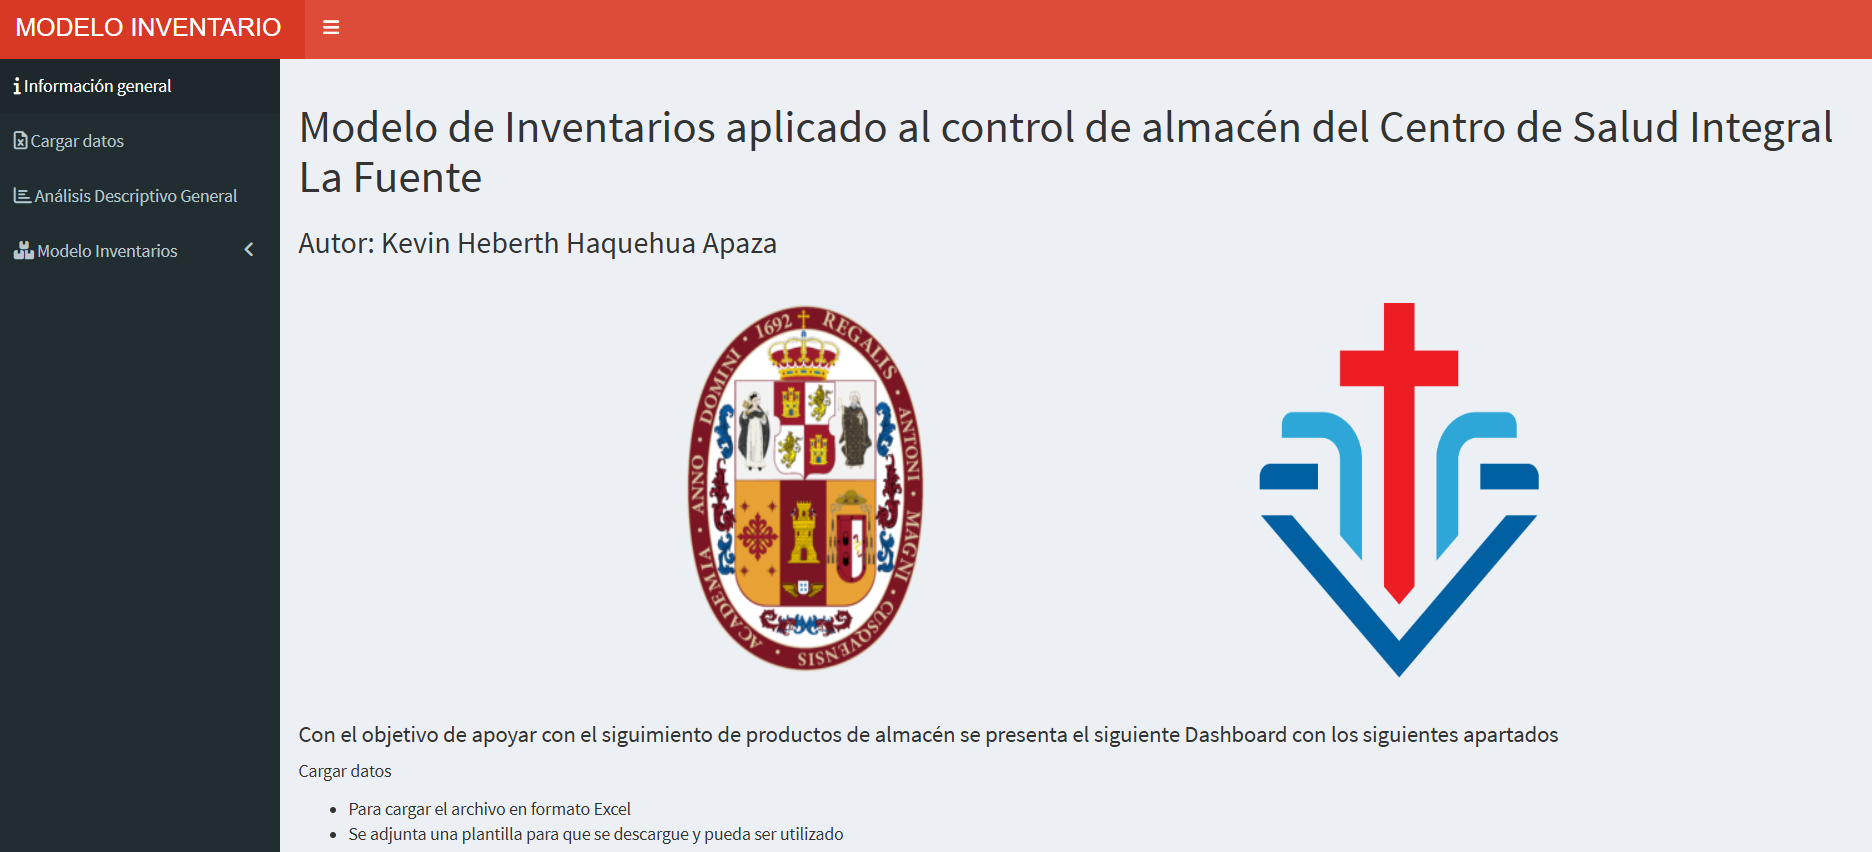
\includegraphics[width=15cm, height=6.85cm]{images/Shiny1.png}}
  \label{fig:Shiny1}
\end{figure}

La Figura \ref{fig:Shiny1} muestra la presentación del aplicativo cuando se accede al enlace proporcionado, asimismo muestra un breve resumen de las funciones que tiene el aplicativo.

\subsection{Cargar datos}
Accediendo a la segunda pestaña del aplicativo ``Cargar datos'', se muestra la parte en donde se tiene que subir los datos para que pueda ser ejecutado el análisis

\begin{figure}[H]
  \caption{Cargar datos del aplicativo de inventario}
  {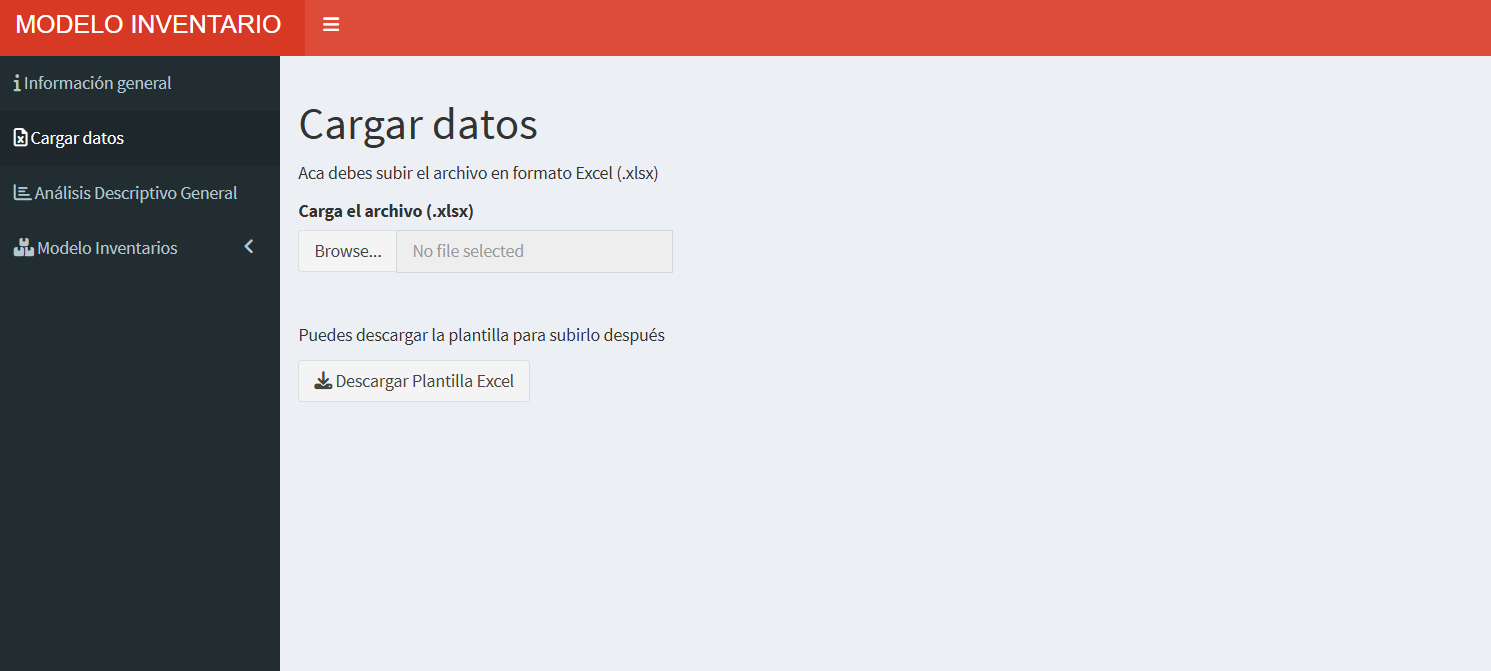
\includegraphics[width=16cm, height=9cm]{images/Shiny2.png}}
  \label{fig:Shiny2}
\end{figure}

La Figura \ref{fig:Shiny2} muestra la sección de cargar datos que viene a ser la primera parte que se debe de realizar, los puntos a tener en cuenta son los siguientes:

\begin{itemize}
  \item La extensión en la que debe subirse el archivo de carga es la extensión \textsl{.xlsx} que viene a ser el formato de archivos Excel.
  \item Asimismo el archivo debe tener dos hojas, en la cual la primera parte debe tener la información de todos los productos: Identificador del producto \textsl{(IDPROD)}, área al que pertenece el producto \textsl{(AREA)}, especialidad al que pertenece el producto \textsl{(ESPECIALIDAD)}, denominación del producto \textsl{(PRODUCTO)}, volumen que ocupa el producto en $cm^3$ \textsl{(VOLUMEN)}, cantidad de pedidos realizados por el producto, aunque este apartado no es tan necesario \textsl{(PEDIDOS)}, costo total del producto en el periodo de tiempo \textsl{(COSTO)}.
  \item La segunda hoja debe tener la demanda de los costos en la cual se debe tener la siguiente información: Identificador del producto el cual debe ser el mismo que el colocado en la primera hoja \textsl{(IDPROD)}, demanda evaluada por el periodo de tiempo (en este caso por meses), volumen que ocupa el producto en $cm^3$ \textsl{(VOLUMEN)}, el costo de compra del producto \textsl{(COSTO\_COMPRA\_C)}, el costo de preparación del producto \textsl{(COSTO\_PREPARACION\_K)}, el costo de retención del producto \textsl{(COSTO\_RETENCION\_h)}, el costo de escasez del producto \textsl{(COSTO\_ESCASEZ\_p)}, tiempo de entrega del pedido \textsl{(TIEMPO\_ENTREGA\_L)}
  \item Una mejor forma de ver el tipo de archivo que se debe subir se puede encontrar en el ANEXO G en donde se muestra la base de datos para realizar el estudio.
  \item De la misma forma en la parte inferior se puede descargar una plantilla con la información solicitada para que se pueda ingresar información y posteriormente subirlo.
  \item Es muy importante que el archivo Excel que se suba al aplicativo contenga la información solicitada que se detalló anteriormente, caso contrario no podrá realizar el análisis y modelos de inventarios.
\end{itemize}

\subsection{Análisis descriptivo general}
Una vez subido el archivo solicitado se tiene que ir a la parte de análisis descriptivo general en donde en base a la primera hoja llenada, mostrará un resumen descriptivo de las áreas y especialidades en base a los costos, y por último mostrará el análisis basado en costos (ABC) de los productos y su categorización.

\subsubsection{Análisis descriptivo por área}
En esta parte se muestra el análisis descriptivo por área tomando principalmente en cuenta los costos.

\begin{figure}[H]
  \caption{Análisis descriptivo general por área del aplicativo de inventario}
  {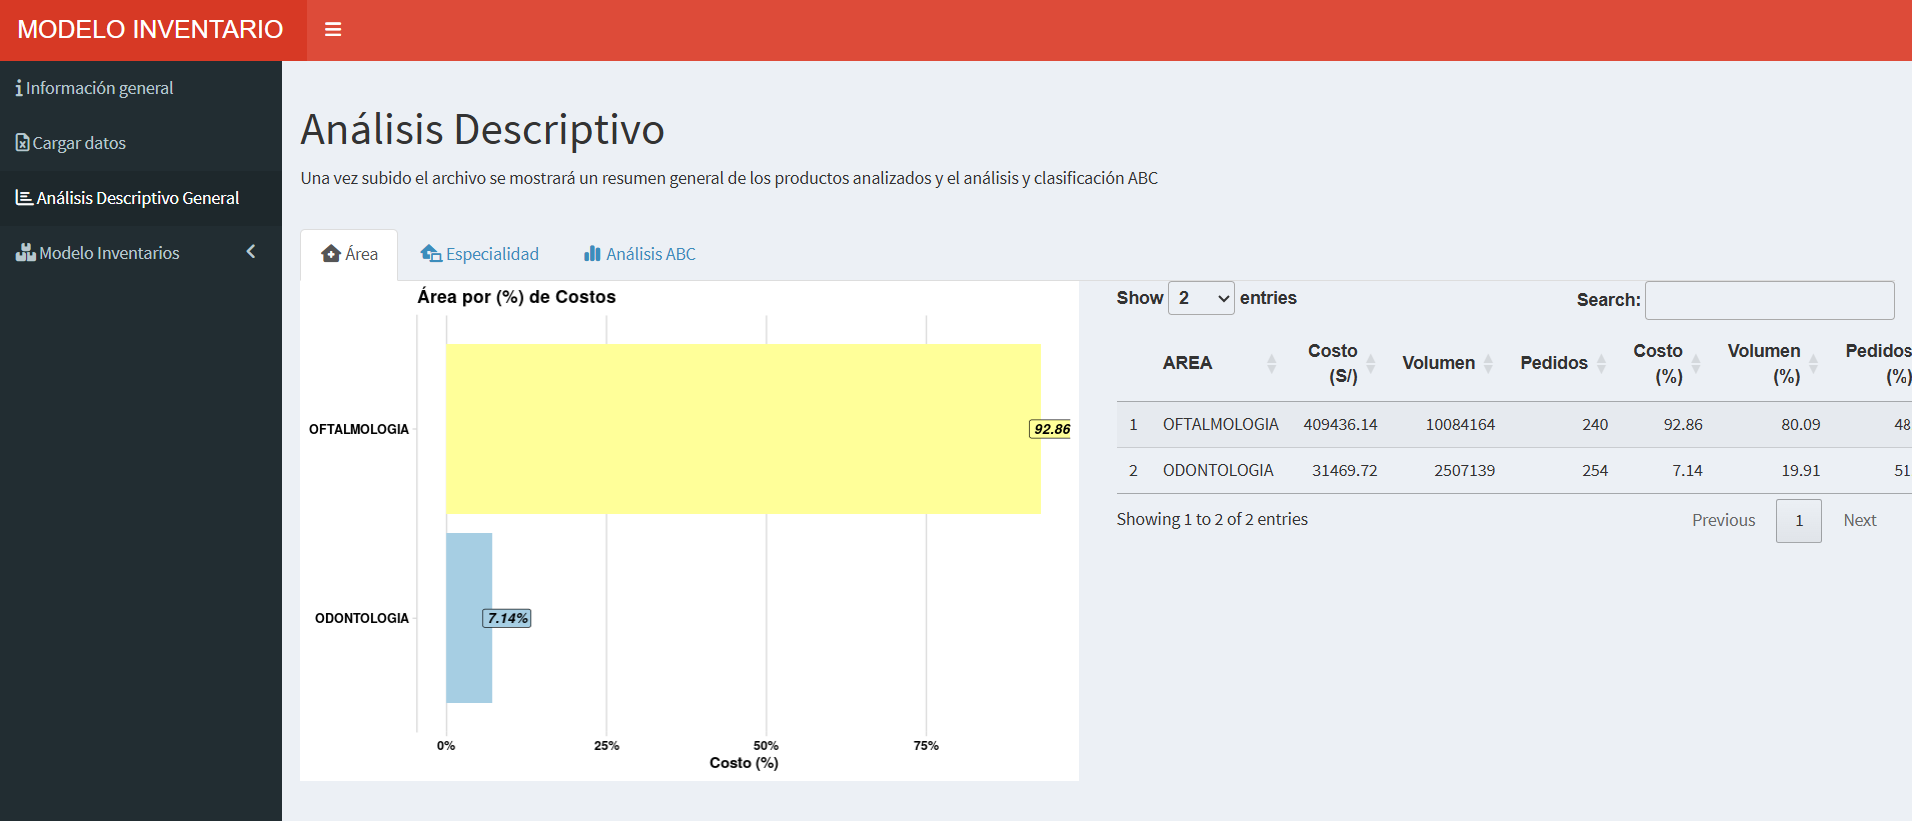
\includegraphics[width=16cm, height=10cm]{images/Shiny3.png}}
  \label{fig:Shiny3}
\end{figure}

La Figura \ref{fig:Shiny3} muestra el análisis por área tomando en cuenta todos los productos, el cual muestra la siguiente información:

\begin{itemize}
  \item En la izquierda se muestra el gráfico de barras que representa las áreas en donde se encuentra la mayor parte de los costos del inventario.
  \item En la derecha se muestra una tabla que resume las áreas tomando en cuenta los costos acumulados, volumen acumulado, pedidos realizados, costos acumulados ($\%$), volumen acumulado ($\%$) y pedidos realizados ($\%$)
\end{itemize}

\subsubsection{Análisis descriptivo por especialidad}
En esta parte se muestra el análisis descriptivo por especialidad tomando principalmente en cuenta los costos.
\clearpage
\begin{figure}[H]
  \caption{Análisis descriptivo general por especialidad del aplicativo de inventario}
  {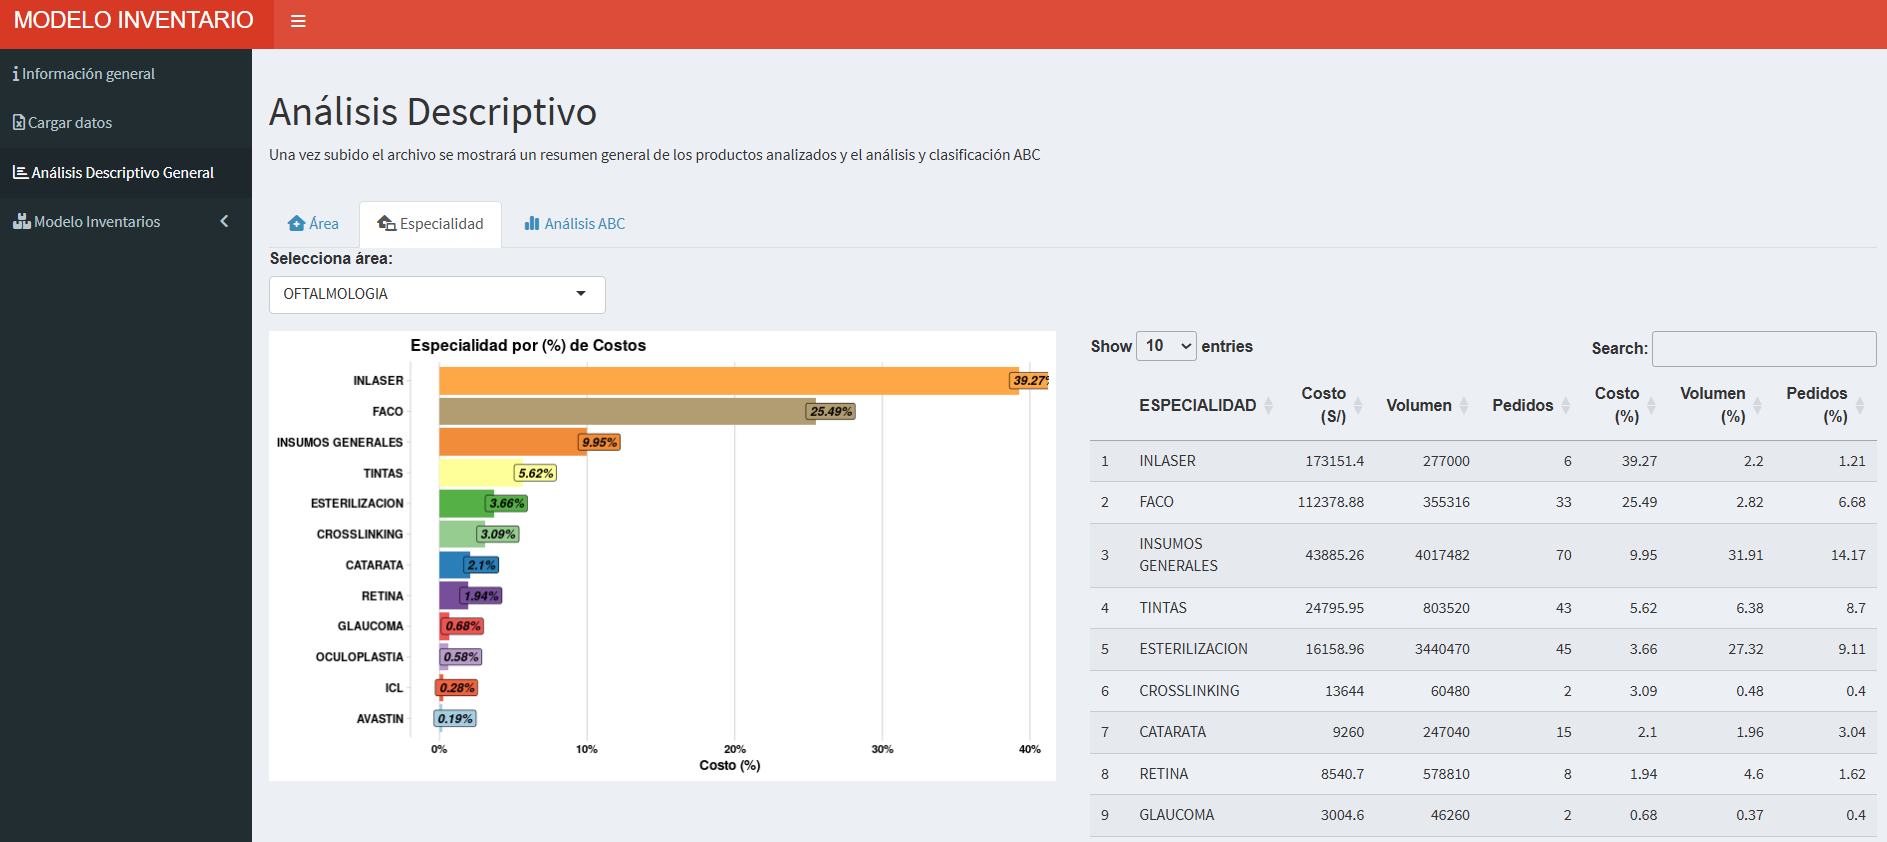
\includegraphics[width=16cm, height=10cm]{images/Shiny4.png}}
  \label{fig:Shiny4}
\end{figure}

La Figura \ref{fig:Shiny4} muestra el análisis por especialidad tomando en cuenta todos los productos, el cual muestra la siguiente información:

\begin{itemize}
  \item Primeramente se tiene un filtro para seleccionar un área y poder ver el análisis.
  \item En la izquierda se muestra el gráfico de barras que representa las especialidades en donde se encuentra la mayor parte de los costos del inventario.
  \item En la parte derecha se muestra una tabla que resume las especialidades tomando en cuenta los costos acumulados, volumen acumulado, pedidos realizados, costos acumulados ($\%$), volumen acumulado ($\%$) y pedidos realizados ($\%$)
\end{itemize}

\subsubsection{Análisis descriptivo por actividades basadas en costos (ABC)}
En esta parte se muestra el análisis de actividades basadas en costos (ABC) el cual el aplicativo es capaz de generar la clasificación de productos mediante la información brindada en los costos.
\clearpage
\begin{figure}[H]
  \caption{Análisis descriptivo de actividades basadas en costos (ABC) del aplicativo de inventario}
  {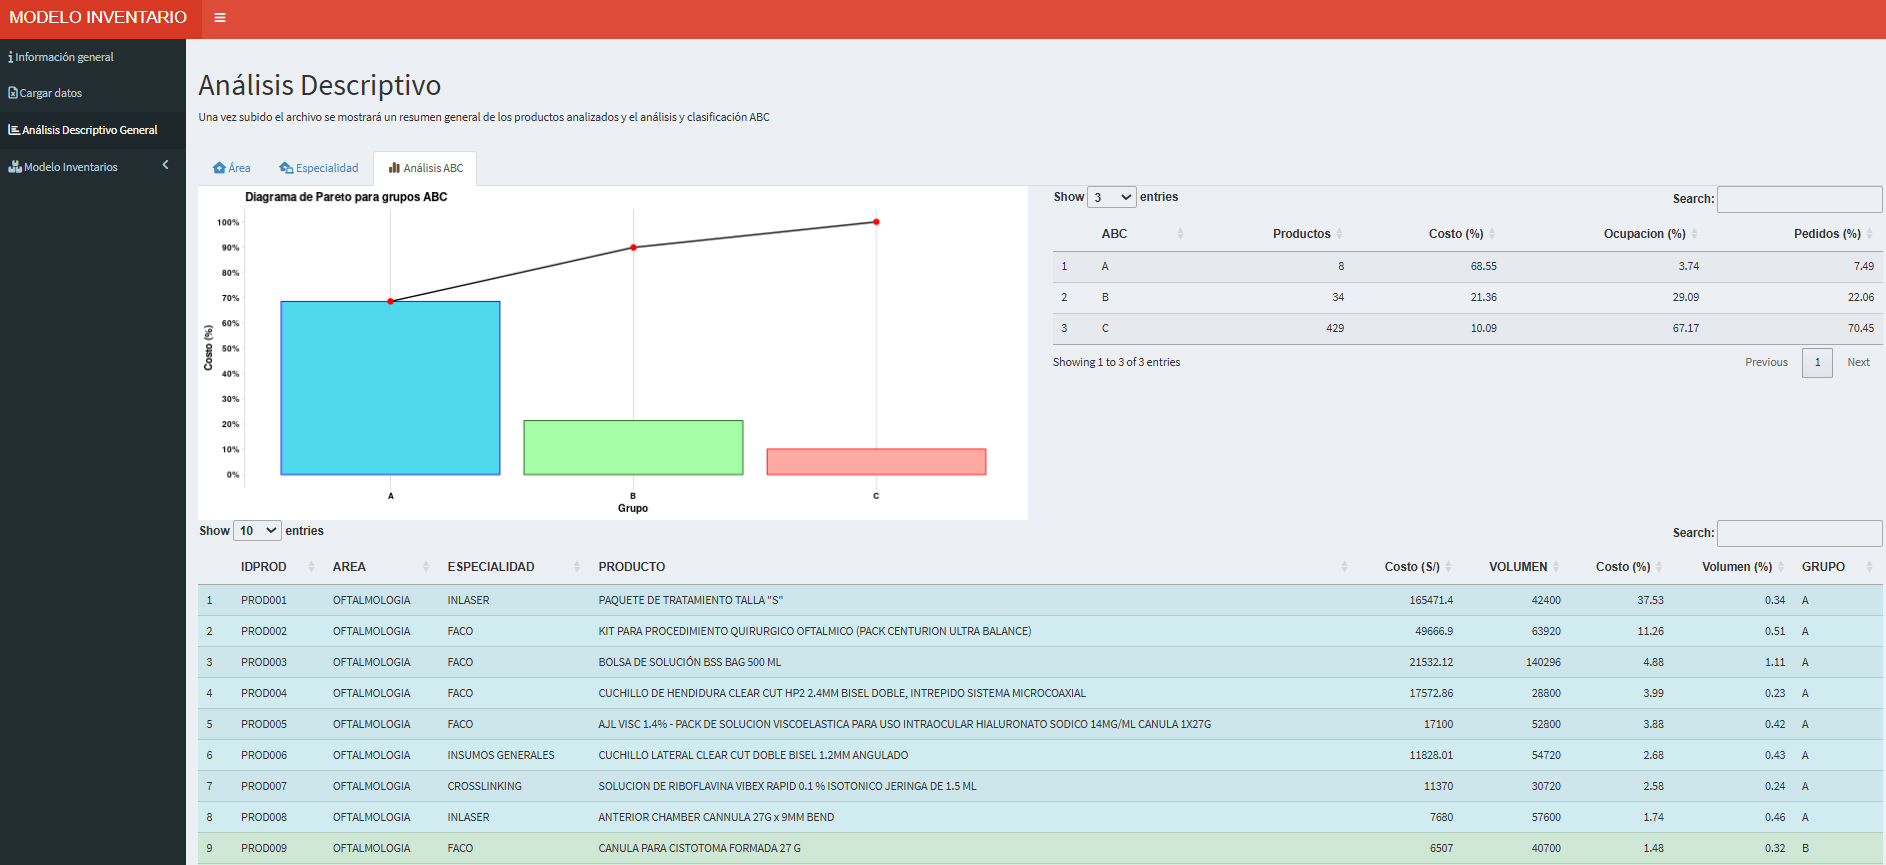
\includegraphics[width=16cm, height=10cm]{images/Shiny5.png}}
  \label{fig:Shiny5}
\end{figure}

La Figura \ref{fig:Shiny5} muestra el análisis de actividades basadas en costos (ABC) tomando en cuenta todos los productos, el cual muestra la siguiente información:

\begin{itemize}
  \item En la izquierda se muestra el diagrama de Pareto que representa los costos por grupos (A, B y C) en porcentaje de los costos.
  \item En la parte derecha se muestra una tabla que resume los resultados obtenidos mediante la clasificación (ABC) tomando en cuenta la cantidad de productos que tiene cada grupo, los costos acumulados ($\%$) en cada grupo, la ocupación que tiene cada grupo ($\%$) y los pedidos realizados por cada grupo ($\%$).
  \item En la parte inferior se muestra la lista de todos los productos, y de la misma forma a que grupo pertenece según la clasificación (ABC)
\end{itemize}
\clearpage
\subsection{Modelo de inventarios determinísticos}

La siguiente parte del análisis que brinda el aplicativo muestra la aplicación de la política de inventarios, primeramente tomando en cuenta los dos modelos determinísticos: EOQ clásico y EOQ con escasez.

\begin{figure}[H]
  \caption{Modelo determinístico del aplicativo de inventario}
  {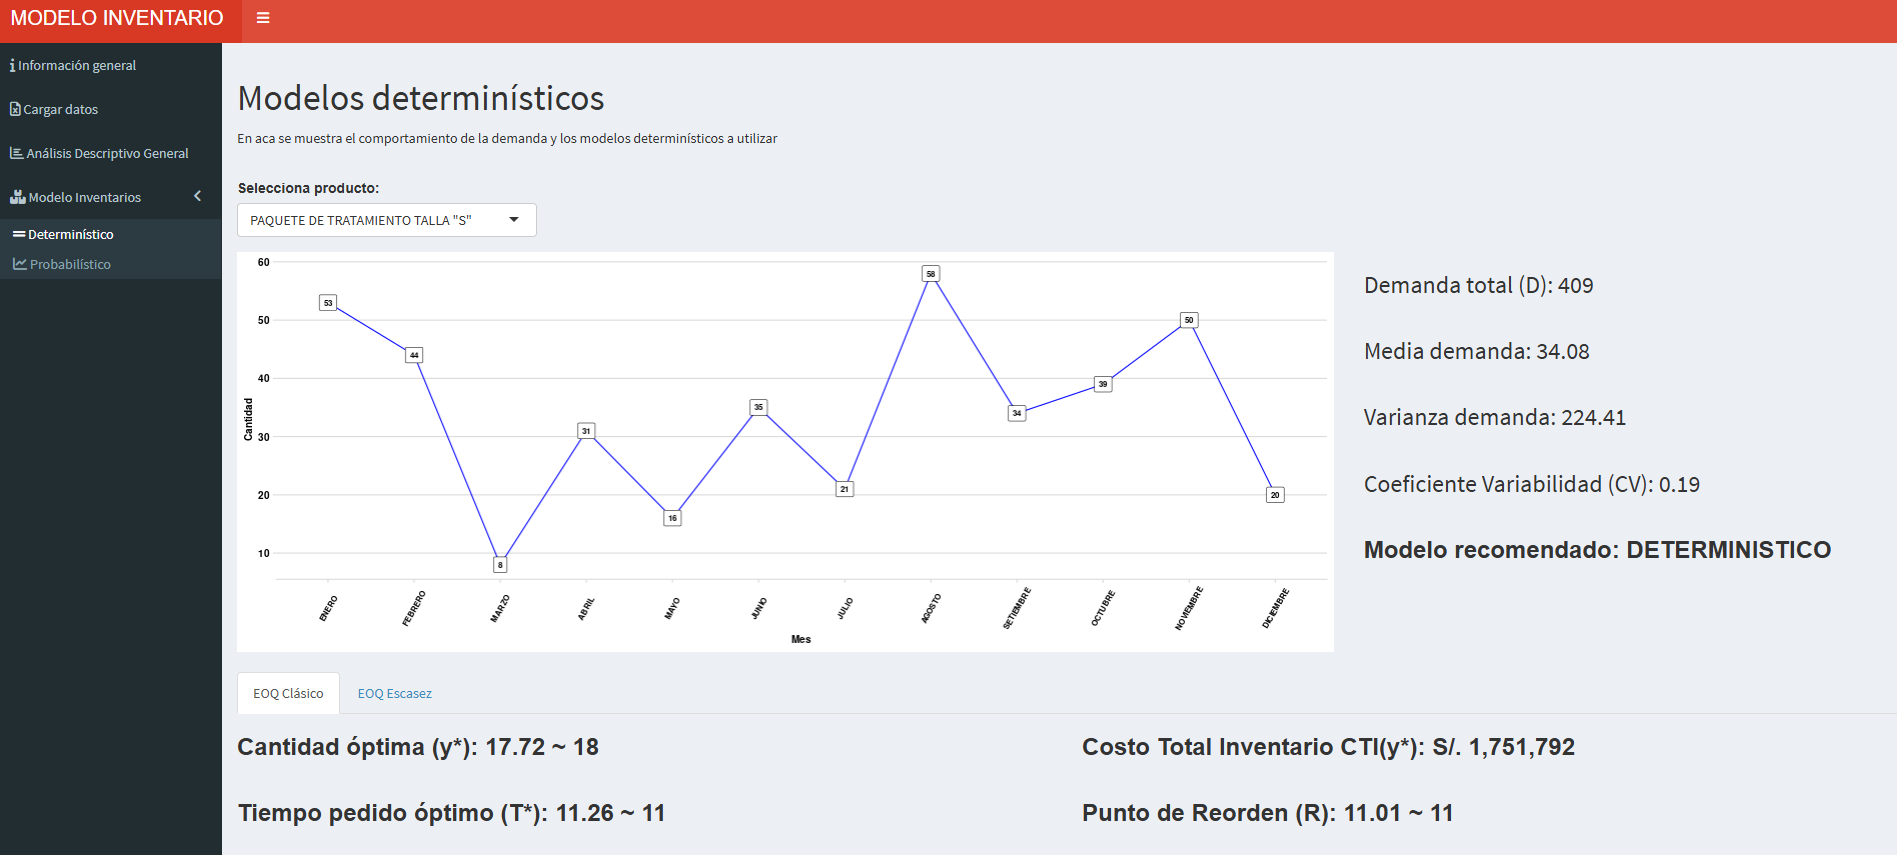
\includegraphics[width=16cm, height=10cm]{images/Shiny6.png}}
  \label{fig:Shiny6}
\end{figure}

La Figura \ref{fig:Shiny6} muestra los resultados de la aplicación del modelo de inventarios determinísticos en la cual se tiene la siguiente información:

\begin{itemize}
  \item En la parte principal se tiene un filtro que selecciona el producto al que se le va a aplicar el análisis y política de inventario óptima.
  \item En la izquierda se muestra un gráfico de línea que representa la demanda del producto por mes.
  \item En la derecha se muestra la información del producto en las cuales se tiene:
  \begin{itemize}
    \item \textbf{Demanda Total (D):} El cual representa la demanda total del periodo analizado, en este caso la demanda anual total.
    \item \textbf{Media demanda:} Representa la media de la demanda tomando en cuenta los periodos, en este caso la media de la demanda mensual.
    \item \textbf{Varianza demanda:} Representa la varianza de la demanda en el periodo analizado, en este caso la varianza de la demanda mensual.
    \item \textbf{Coeficiente de variabilidad (CV):} Representa el coeficiente de variabilidad calculado para ver si el modelo a usar es un determinístico ($CV < 0.20$) o un probabilístico ($CV \geq 0.20$).
    \item \textbf{Modelo recomendado:} Indica el modelo recomendado a utilizar (determinístico o probabilístico) tomando en cuenta el coeficiente de variabilidad.
  \end{itemize}
\end{itemize}


\subsubsection{Modelo clásico de cantidad económica de pedido (EOQ)}
La primera parte muestra los resultados aplicando el modelo determinístico EOQ clásico tomando en cuenta la información brindada en la sección (\ref{Modelo_clas_EOQ}) el cual muestra la siguiente información

\begin{itemize}
  \item \textbf{Cantidad óptima ($y^*$):} Muestra la cantidad óptima de pedido calculado mediante el modelo.
  \item \textbf{Tiempo pedido óptimo ($T^*$):} Muestra el tiempo de pedido óptimo para realizar el pedido del modelo.
  \item \textbf{Costo total inventario ($CTI(y^*)$):} Muestra el costo total que se obtendrá con la aplicación del modelo.
  \item \textbf{Punto de reorden (R):} Muestra el punto en la que debe de realizarse el siguiente pedido.
\end{itemize}

\subsubsection{Modelo clásico de cantidad económica de pedido (EOQ) con escasez}

La segunda parte muestra los resultados aplicando el modelo determinístico EOQ clásico con escasez, a pesar de que en los resultados obtenidos de los productos analizados no se tuvieron costos de escasez, es necesario colocar este análisis ya que el centro de salud puede agregar otros productos que necesite analizar su política de inventarios y tenga estos costos, para los resultados de este análisis se toma en cuenta la información de la sección (\ref{EOQ_escasez}) y seleccionando en el aplicativo la pestaña de EOQ Escasez.

\begin{figure}[H]
  \caption{Modelo determinístico EOQ con escasez del aplicativo de inventario}
  {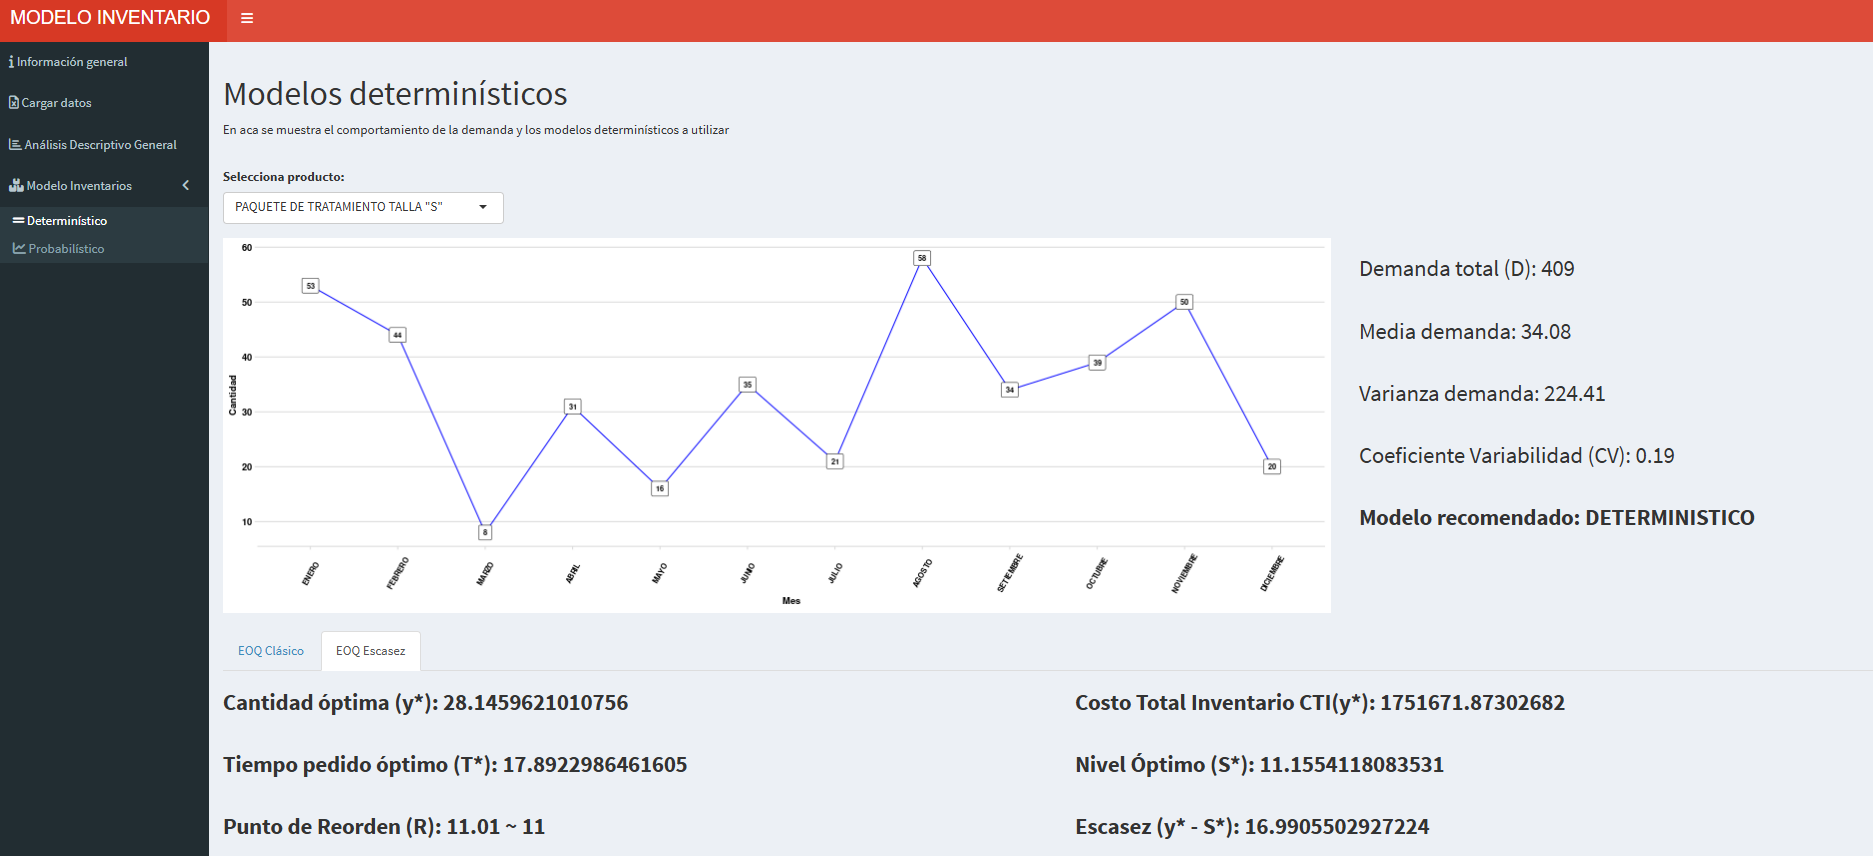
\includegraphics[width=16cm, height=10cm]{images/Shiny7.png}}
  \label{fig:Shiny7}
\end{figure}

La Figura \ref{fig:Shiny7} muestra los resultados tomando en cuenta el modelo EOQ con escasez, para mostrar el ejemplo se agrego al primer producto analizado un costo de escasez de S/ 6.50 en el cual la primera parte muestra la información general del modelo determinístico, la segunda parte muestra lo siguiente:

\begin{itemize}
   \item \textbf{Cantidad óptima ($y^*$):} Muestra la cantidad óptima de pedido calculado mediante el modelo.
  \item \textbf{Tiempo pedido óptimo ($T^*$):} Muestra el tiempo de pedido óptimo para realizar el pedido del modelo.
  \item \textbf{Costo total inventario ($CTI(y^*)$):} Muestra el costo total que se obtendrá con la aplicación del modelo.
  \item \textbf{Punto de reorden (R):} Muestra el punto en la que debe de realizarse el siguiente pedido.
  \item \textbf{Nivel Óptimo ($S^*$):} Muestra el nivel óptimo de inventario que se debe tener tomando en cuenta el modelo.
  \item \textbf{Nivel de escasez óptimo ($y^* - S^*$):} Muestra el nivel de escasez óptimo permitido aplicando el modelo.
\end{itemize}

\subsection{Modelo probabilístico}
La última parte que brinda el aplicativo es el análisis aplicando el modelo probabilístico usando la información brindada en la sección (\ref{EOQ_probabilizado}) el cual usa el modelo EOQ clásico tomando un nivel de reserva basándose en que la demanda se puede expresar mediante una distribución normal estándar, a pesar de que el coeficiente de variabilidad calculado indica que solo es necesario usar los modelos determinísticos, el centro de salud necesitaría también tomar en cuenta este modelo, especialmente para nuevos productos en los cuales se tenga un comportamiento probabilístico.

\begin{figure}[H]
  \caption{Modelo determinístico EOQ probabilizado del aplicativo de inventario}
  {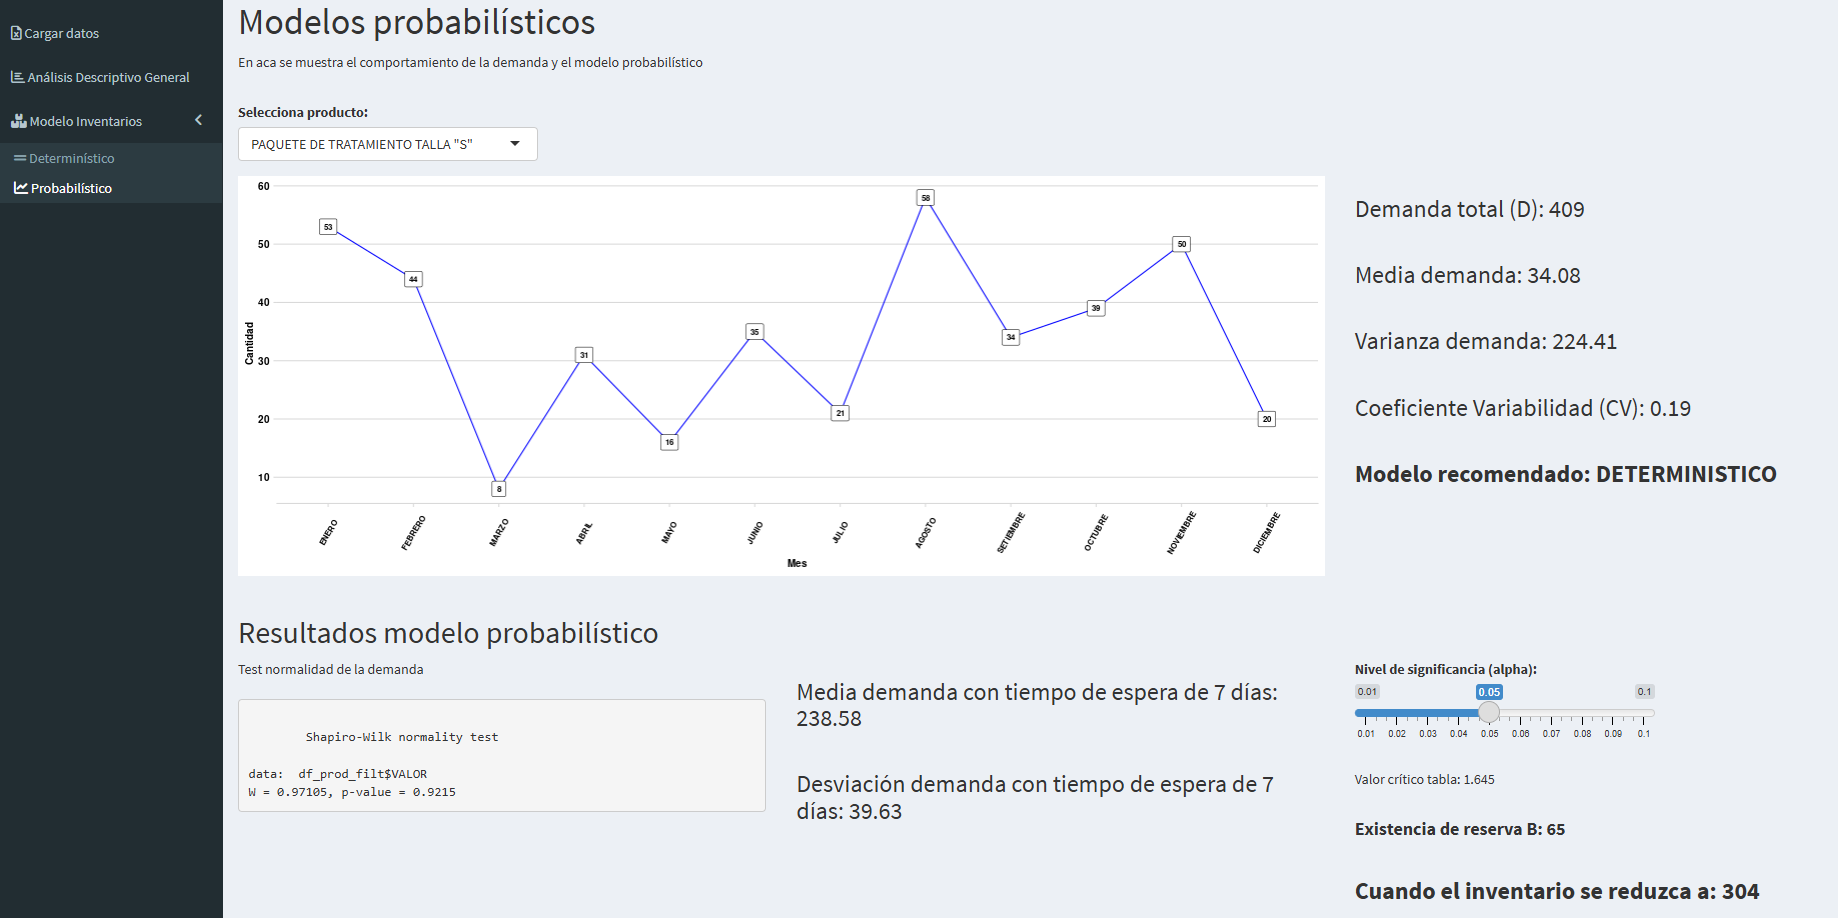
\includegraphics[width=16cm, height=9cm]{images/Shiny8.png}}
  \label{fig:Shiny8}
\end{figure}
\clearpage
La Figura \ref{fig:Shiny8} muestra los resultados obtenidos mediante el modelo probabilizado de la cantidad de pedido, la primera parte muestra los mismos resultados obtenidos en los modelos determinísticos, mientras que en la parte inferior se muestra la siguiente información:

\begin{itemize}
  \item \textbf{Test de normalidad de la demanda:} En esta parte muestra los resultados del test de normalidad usando la prueba de Shapiro-Wilk hacia el comportamiento de la demada, en el cual planteando un nivel de significancia y observado el p-value se decide por aceptar o rechazar la hipótesis nula ($H_0$) acerca de que la demanda mensual se aproxima a una distribución normal.
  \item \textbf{Media demanda con tiempo de espera:} Indica la media de la demanda con respecto al tiempo de entrega.
  \item \textbf{Desviación demanda con tiempo de espera:} Indica la desviación de la demanda con respecto al tiempo de entrega.
  \item \textbf{Nivel de significancia ($\alpha$):} Indica el nivel de significancia que se debe colocar para realizar el cálculo de la cantidad de pedido óptimo.
  \item \textbf{Existencia de reserva ($B$):} Muestra la cantidad de existencia de reserva calculado por el modelo.
  \item \textbf{Nivel de inventario para realizar el pedido:} Indica el momento para realizar el pedido, cuando el inventario llegue a las unidades del modelo se debe de realizar el siguiente pedido.
\end{itemize}

